% DER_XVI: Grothendieck's text with the commentary set in, then the overview, inside a group that applies the chunk's own definitions
\dgrchapter{XVI}{Chapter XVI}{Les localiseurs fondamentaux}
\dgrpart{0}{XVI}{Manuscript pages 1--124}{XVI\enspace\textperiodcentered\enspace Chapter XVI\enspace\textperiodcentered\enspace manuscript pages 1--124}{Chapter XVI \textperiodcentered\ \textup{XVI}}
\dgrchunkbegin
% DER_XVI: the definitions of the chunk's preamble, applied inside its group
\let\printedpage\relax\newcommand{\printedpage}[1]{\marginpar{\footnotesize p.~#1}}
\let\msp\relax\newcommand{\msp}[1]{\marginpar{\footnotesize [#1]}}
\let\circled\relax\newcommand{\circled}[1]{\tikz[baseline=(c.base)]\node[draw,circle,inner sep=1pt](c){#1};}
\let\Cat\relax\newcommand{\Cat}{\mathrm{Cat}}
\let\Ob\relax\newcommand{\Ob}{\mathrm{Ob}\,}
\let\hot\relax\newcommand{\hot}{\mathrm{hot}}
\let\Loc\relax\newcommand{\Loc}{\mathrm{Loc}}
\let\Hom\relax\newcommand{\Hom}{\operatorname{Hom}}
\let\Fl\relax\newcommand{\Fl}{\operatorname{Fl}}
\let\Hot\relax\newcommand{\Hot}{\mathrm{Hot}}
\let\Ens\relax\newcommand{\Ens}{\mathrm{Ens}}
\let\id\relax\newcommand{\id}{\mathrm{id}}
\let\Cof\relax\newcommand{\Cof}{\mathrm{Cof}}
\let\Mono\relax\newcommand{\Mono}{\mathrm{Mono}}
\let\univ\relax\newcommand{\univ}{\mathrm{univ}}
\let\Fib\relax\newcommand{\Fib}{\mathrm{Fib}}
\let\Fibf\relax\newcommand{\Fibf}{\mathrm{Fibf}}
\let\Parf\relax\newcommand{\Parf}{\mathrm{Parf}}
\let\Catfib\relax\newcommand{\Catfib}{\mathrm{Catfib}}
\let\Fibsc\relax\newcommand{\Fibsc}{\mathrm{Fibsc}}
\let\HOT\relax\newcommand{\HOT}{\mathrm{HOT}}
\let\cF\relax\newcommand{\cF}{\mathcal{F}}
\let\cM\relax\newcommand{\cM}{\mathcal{M}}
\let\Comp\relax\newcommand{\Comp}{\mathrm{Comp}}
\let\dottedimplies\relax\newcommand{\dottedimplies}{\mathrel{\tikz[baseline=-0.6ex]{\draw[dotted, double, double distance=1.5pt, -{Implies}] (0,0) -- (0.9,0);}}}
\let\inc\relax\newcommand{\inc}{\mathrm{inc}}
\let\dotimp\relax\newcommand{\dotimp}{\overset{\bullet}{\Longrightarrow}}
\let\dottedimpl\relax\newcommand{\dottedimpl}{\mathrel{\begin{tikzcd}[ampersand replacement=\&, column sep=small, baseline=-0.5ex]{}\arrow[r,Rightarrow,dotted]\&{}\end{tikzcd}}}
\let\cercle\relax\newcommand{\cercle}[1]{\tikz[baseline=(c.base)]\node[draw,circle,inner sep=1pt](c){#1};}
\let\fourche\relax\newcommand{\fourche}{\begin{tikzcd}[ampersand replacement=\&, row sep=0.5em, column sep=1em, baseline=(\tikzcdmatrixname-2-1.base)]\& X_1 \\ X_0 \arrow[ur]\arrow[dr] \& \\ \& X_2\end{tikzcd}}
\let\carre\relax\newcommand{\carre}{\begin{tikzcd}[ampersand replacement=\&, row sep=0.5em, column sep=1em, baseline=(\tikzcdmatrixname-2-1.base)]\& X_1 \arrow[dr] \& \\ X_0 \arrow[ur]\arrow[dr] \& \& X \\ \& X_2 \arrow[ur] \&\end{tikzcd}}
\let\uFl\relax\newcommand{\uFl}{\underline{\mathrm{Fl}}}
\let\uCat\relax\newcommand{\uCat}{\underline{\mathrm{Cat}}}

% ---- from der-ch16_p001-005.tex
% ===================== page 1 (PDF) =====================
\printedpage{[non numérotée]}
% head: (none printed)

\begin{center}
{\sffamily\LARGE LES DÉRIVATEURS}

\bigskip

{\large\textbf{ALEXANDRE GROTHENDIECK}}

\vspace{3em}

{\large\textbf{Chapitre XVI}}

\medskip

{\large\textbf{Les localiseurs fondamentaux}}
\end{center}

\clearpage

% ===================== page 2 (PDF) =====================
\printedpage{[non numérotée]}
% head: (none printed)

Ce texte a été déchiffré et transcrit en \LaTeXe{} par M. Künzer. Il a été édité par M. Künzer, J. Malgoire, et G. Maltsiniotis. La transcription est aussi fidèle que possible au manuscrit. Seules quelques corrections mineures évidentes ont été effectuées. Pour les rares ajouts ou commentaires des éditeurs, ainsi que pour la numérotation originale des pages du manuscrit, les caractères de machine à écrire \texttt{[typewriter]} entre crochets sont utilisés.

Cette édition est provisoire. Les remarques, commentaires et corrections sont bienvenus. Envoyer un message à :

\textbf{[e-mail address removed]}

\hfill G. Maltsiniotis\hspace*{2cm}

\clearpage

% ===================== page 3 (PDF) =====================
\printedpage{1}
% head: A. Grothendieck : Dérivateurs, Ch. XVI, Édition des Universités de Montpellier II et Paris VII
% foot: Version 18 mars 2019

\msp{page 1}

\section*{1\quad Axiomes Loc(1) à Loc(3) (et variantes) : localiseurs fondamentaux}

J’ai envie de reprendre l’exposé des axiomes utiles pour un localiseur fondamental
\[
W \subset \mathrm{Fl}(\Cat),
\]
en me guidant cette fois plus sur la signification géométrique des axiomes, que sur les alias $\pm$ techniques qu’on rencontre (ou ne rencontre pas) pour les vérifier. Je révise donc dans cet esprit la présentation de XV §9.

\begin{description}
\item[Loc (1)] (\textit{saturation}).
\begin{itemize}
\item[\textit{a})] Iso $\subset W$.
\item[\textit{b})] Si deux parmi $f$, $g$, $gf$ sont dans $W$, aussi le troisième.
\item[\textit{c})] Si $gf$ et $fg$ sont dans $W$, $f$ et $g$ aussi.
\end{itemize}
\end{description}

Les conditions (\textit{a}) et (\textit{b}) toutes seules, je vais les appeler (pour un $W \subset \mathrm{Fl}\,\mathcal{M}$ général) \textit{saturation faible} du localiseur. Les conditions (\textit{a}), (\textit{b}), (\textit{c}), \textit{saturation modérée} (“mild saturation”). Autres variantes :

\begin{description}
\item[Loc (1 bis)] Les conditions (\textit{a}), (\textit{b}), (\textit{c}) du haut, plus
\begin{itemize}
\item[\textit{d})] $W$ stable par facteurs directs.
\end{itemize}
\end{description}

C’est bien sûr impliqué par :

\begin{description}
\item[Loc (1 ter)] $W$ est \textit{fortement saturé, i.e.} si $f \in \Cat$ est telle que $\hot_W(f)$ est un isomorphisme, alors $f \in W$.
\item[Loc (2)] (\textit{Objet final}). Si $X$ dans Cat a un objet final, alors $X$ est $W$-asphérique, \textit{i.e.} $X \longrightarrow e$ est dans $W$.
\end{description}

Parfois, cet axiome est conséquence de la variante affaiblie suivante.

\begin{description}
\item[Loc (2$_0$)] (Axiome du segment). $\boldsymbol{\Delta}^1$ est $W$-asphérique.
\end{description}

\msp{page 2}

\begin{description}
\item[Loc (3)] (\textit{localisation,} forme faible). Soit $f : X \longrightarrow S$ une flèche dans Cat $W$\textit{-asphérique, i.e.} telle que $\forall\ s \in \Ob S$, la catégorie localisée $X/s$ sur $S$ en $s$, $X/s = X \times_S S/s$, soit $W$-asphérique. Alors $f \in W$.\footnote[1]{Dans une version finale, il faudrait intervertir les notations pour Loc (3) et pour Loc (3 bis), car ce dernier m’apparaît comme le plus important des deux - il est satisfait pour tous les localiseurs qui ont été utilisées (à ma connaissance), et est valable pour tout localiseur de la forme $W_{\mathbf{D}}$, où $\mathbf{D}$ est un dérivateur (ou seulement un prédérivateur satisfaisant Der (4,5) \texttt{[il faut aussi Der (2) ; la numérotation des axiomes est celle du chapitre I, p. 68]}).} % mark printed as superscript (1); [sic] utilisées -> utilisés, agreement with "localiseurs"
\end{description}

\textbf{Rappel 1.} Loc (1, 2, 3) impliquent que l’on a
\[
W = W^\circ \qquad \textit{i.e. } f \in W \iff f^\circ \in W,
\]
\printedpage{2}
% head: A. Grothendieck : Dérivateurs, Ch. XVI, Édition des Universités de Montpellier II et Paris VII
% foot: Version 18 mars 2019
où on dénote par $X \longmapsto X^\circ$, $f \longmapsto f^\circ$ le foncteur de passage à la catégorie opposée, foncteur
\[
X \longmapsto X^\circ : \Cat \xrightarrow{\ \sim\ } \Cat
\]
qui est un \textit{automorphisme} de Cat (donc commute à toutes $\varinjlim$ et $\varprojlim$ ). Il s’ensuit que l’ensemble d’axiomes Loc (1, 2, 3) équivaut à Loc (1, 2$^{\mathrm{opp}}$, 3$^{\mathrm{opp}}$), où Loc (2$^{\mathrm{opp}}$) est l’axiome “dual” de Loc (2), savoir que tout objet de Cat ayant un objet initial est $W$-asphérique, et de même Loc (3$^{\mathrm{opp}}$) l’axiome que toute $f : X \longrightarrow S$ $W$\textit{-coasphérique, i.e.} telle que les catégories colocalisées $s\backslash X$ de $X$ sur $S$ soient $W$-asphériques, est dans $W$.

\textbf{Définition 1.1.} On appelle \textit{localiseur fondamental} une partie $W$ de Fl(Cat) satisfaisant les axiomes Loc (1, 2, 3) (\textit{i.e.} saturation modérée, axiome de l’objet final, axiome de localisation).

\msp{page 3}

\dgrblock{dgrb835}{Axioms for equivalences before a choice of model}
\begin{dcomment}{context}{p2}{Axioms for equivalences before a choice of model}
\textit{Commentary and mathematical audit AI-produced by GPT-6 Astra (OpenAI, ChatGPT Pro mode), checked and integrated by Claude (Anthropic).}

Grothendieck starts with a class of functors, rather than with cofibrations and fibrations. The distinction matters throughout this chapter: the latter classes are to be recovered, when possible, from stability properties of the former. His letter to Thomason of 2 April 1991, \S1, describes precisely this separation between the equivalences carrying the homotopy theory and the auxiliary devices used to calculate it \citep{Grothendieck1991Letter}. Here the basic datum is a class $W$ in $\Cat$; the localization $L:\Cat\to\Hot_W$ exists in the chosen larger universe and need not come with a calculus of single fractions.

Three meanings of saturation must consequently remain distinct. The two-out-of-three property controls a composable pair. The extra condition (1c) controls a pair $f:A\to B$, $g:B\to A$ when both composites are already equivalences. It is just what is needed to recognize a homotopy inverse before one knows that every arrow inverted by $L$ belongs to $W$. Closure under retracts is an additional requirement here. Strong saturation means $W=L^{-1}(\operatorname{Iso})$; it implies retract closure because an arrow which is a retract of an isomorphism is an isomorphism. One cannot substitute strong saturation silently in arguments made under (1).

There is also a consequential change of terminology in the later literature. Definition 1.1 calls the class satisfying (1,2,3) a fundamental localizer. Later authors generally call this a \emph{weak} fundamental localizer and reserve the unqualified name for the relative axiom (3 bis). The distinction concerns the hypothesis of Theorem A, not merely a word. In (3), the comma categories $X/s$ are individually aspherical. In (3 bis), the two comma categories may each have substantial homotopy, provided that the comparison between them is an equivalence. The latter implication does not follow by applying the former separately to $X\to S$ and $Y\to S$.

The editor's addition of Der (2) in footnote 1 is therefore mathematically substantive. A pointwise comparison of diagram objects gives an isomorphism only when the evaluations detect isomorphisms. The derivator axioms numbered here are those of Chapter I; importing a modern numbering without translating it would conceal the missing conservativity assumption. This is the same point already isolated in the commentary to XIIa on constructing localizers from derivators.
\end{dcomment}


\textbf{Rappel 1.2.} Si $W$ est un localiseur fondamental, alors tout \textit{homotopisme} $f : X \longrightarrow Y$ de Cat est dans $W$ (c’est pour cela essentiellement que l’on a imposé (\textit{c}) dans la saturation modérée Loc (1)). Si $f, g : X \rightrightarrows Y$ sont homotopes (\textit{i.e.} appartiennent à une même composante connexe de $\underline{\mathrm{Hom}}(X, Y)$), alors $\hot_W(f) = \hot_W(g)$ et $f \in W \iff g \in W$.

Voici la forme forte de Loc (3).

\begin{description}
\item[Loc (3 bis)] (\textit{Localisation,} forme forte). Soit $S$ dans Cat et $f : X \longrightarrow Y$ un morphisme dans $\Cat/S$ tel que “$f$ soit une $W$-équivalence localement sur $S$”, \textit{i.e.} pour tout $s \in \Ob S$, le morphisme induit
\[
f/s : X/s \longrightarrow Y/s
\]
pour les catégories localisées de $X$, $Y$ sur $S$ en $s$, soit dans $W$. Alors $f \in W$.
\end{description}

L’axiome Loc (3) n’est autre que le cas particulier de Loc (3 bis) relatif au cas où $Y = S$.

\textbf{Proposition 1.3.} \textit{Soit $W \subset \mathrm{Fl}(\mathcal{M})$. Alors on a les équivalences suivantes}
\[
\begin{aligned}
\text{Loc (1, 2, 3)} &\iff \text{Loc (1, $2_0$, $3'$)}\\
\text{Loc (1, 2, 3 bis)} &\iff \text{Loc (1, $2_0$, $3'$ bis),}
\end{aligned}
\]
\textit{où les axiomes} Loc ($3'$) \textit{et} Loc ($3'$ bis) \textit{se formulent ainsi :}

\msp{page 4}

\begin{description}
\item[Loc (3$'$)] \circled{\textit{a}} (Axiome des Cat-fibrations, forme directe faible). Soient $S$ dans Cat, $X$ une catégorie fibrée scindée sur $S$, telle que les fibres $X_s$ ($s \in \Ob S$) soient $W$-asphériques. Alors $X \longrightarrow S$ est dans $W$.

\circled{\textit{b}} Soit $X$ dans $\Cat/S$, alors $i_X : X \longrightarrow \Phi_S(X)$ est dans $W$\footnote[2]{(\textit{b}) concerne la \textit{comparaison} d’une $X$ quelconque sur $S$, avec la catégorie fibrée scindée $\Phi_S(X)$ sur $S$.}. % mark printed as superscript (2)
\end{description}

\clearpage

% ===================== page 5 (PDF) =====================
\printedpage{3}
% head: A. Grothendieck : Dérivateurs, Ch. XVI, Édition des Universités de Montpellier II et Paris VII
% foot: Version 18 mars 2019

\begin{description}
\item[Loc (3$'$ bis)] \circled{\textit{a}} (Axiome des Cat-fibrations, forme directe forte). Soient $S$ dans Cat, $X$, $Y$ deux catégories fibrées scindées sur $S$, $f : X \longrightarrow Y$ un $S$-foncteur cartésien compatible aux scindages, tel que $\forall\ s \in \Ob S$, le foncteur induit sur les fibres
\[
f_s : X_s \longrightarrow Y_s
\]
soit dans $W$. Alors $f \in W$.

\circled{\textit{b}} Comme Loc ($3'$) (\textit{b}).
\end{description}

\textbf{N.B.} En fait, moyennant Loc (1, 2), les énoncés Loc ($3'$), Loc ($3'$ bis) impliquent les énoncés similaires sans scindages, et sans même supposer $f$ cartésien dans Loc ($3'$ bis), \textit{cf.} démonstration ci-dessous.

\textsc{Démonstration.} \textit{a}) Loc (1, 2, 3) $\Longrightarrow$ Loc (1, $2_0$, $3'$). Il suffit de prouver Loc ($3'$). Prouvons Loc ($3'$ $a$). Pour ceci, sous les conditions de Loc ($3'$ $a$), prouvons que $X \longrightarrow S$ est $W$-coasphérique, \textit{i.e.} que les catégories
\[
s\backslash X = X \times_S s\backslash S
\]
sont $W$-asphériques. Il en résultera bien que $f \in W$ en vertu de Loc (3) appliqué à $f^\circ$ et de $W = W^\circ$. Mais
\msp{page 5}
considérons l’inclusion canonique
\[
i_s : X_s \lhook\joinrel\longrightarrow s\backslash X,
\]
il résulte du fait que $p : X \longrightarrow S$ est Cat-fibrant que ce foncteur est $W$-asphérique (il a même un adjoint à droite, \textit{i.e.} les catégories $X_s/u$, où $u \in \Ob(s\backslash X)$, ont un objet final). Donc par Loc (3) on a $i_s \in W$, et comme $X_s$ est $W$-asphérique par hypothèse, de même $s\backslash X$, q.e.d.

\dgrblock{dgrb836}{Comma categories replace a map by a fibration}
\begin{dcomment}{exposition}{p4}{Comma categories replace a map by a fibration}
The construction $\Phi_S(X)$ makes Proposition 1.3 transparent. For $p:X\to S$, its objects can be written
\[
(s,x,\alpha:s\longrightarrow p(x)).
\]
A morphism to $(t,y,\beta)$ is a pair $(h:s\to t,k:x\to y)$ satisfying $p(k)\alpha=\beta h$. Projection to $s$ is a split Grothendieck fibration; reindexing along $h:s\to t$ replaces $(t,y,\beta)$ by $(s,y,\beta h)$. Thus its fibre over $s$ is $s\backslash X$. The inclusion
\[
i_X(x)=(p(x),x,\id_{p(x)})
\]
has left adjoint $q(s,x,\alpha)=x$: a map from $(s,x,\alpha)$ to $i_X(y)$ is determined uniquely by $k:x\to y$. In particular, $qi_X=\id_X$, and the unit supplies the other homotopy. This explains the comparison axiom (3$'$b), including the direction of its adjoint.

If $p:X\to S$ is itself a fibration, the inclusion $X_s\to s\backslash X$ has a right adjoint: choose the cartesian pullback $\alpha^*x$ of $x$ along $\alpha:s\to p(x)$. The adjunction follows from the defining universal property of a cartesian arrow. Its comma categories have terminal objects, so (2) and (3) put the inclusion in $W$. Consequently the fibrewise hypothesis can be transferred to the comma categories. This is the sole place where the fibration condition is doing work; a general functor's strict fibres need not compute the comma categories.

For example, take $S=(0\to1)$ and let $X=e$ map to $1$. The strict fibre over $0$ is empty, although $0\backslash X=e$. Replacing $X$ by $\Phi_S(X)$ produces $S$ itself. A condition on strict fibres of an arbitrary map would incorrectly reject this contractible example; the replacement repairs exactly that defect.

The reverse implication in the proposition first gets $\Delta^1\times X\to X$ from the fibre axiom and the segment axiom. The two endpoint inclusions become equal inverses after localization. A natural transformation therefore makes its endpoint functors equal in $\Hot_W$, and two-out-of-three gives the corresponding equivalence of membership in $W$. For a homotopy equivalence, (1c) then recognizes the two inverse functors as members of $W$. A category with a final or initial object is contractible by these natural transformations, which recovers (2). Finally the displayed square involving $\Phi_S(f)$ transfers the relative fibre condition back to $f$. This proof also explains why a chosen splitting and preservation of its cartesian arrows are unnecessary in the final fibrewise criterion: the comparison with the comma categories works for every functor over $S$ between fibrations. For the later systematic separation of fibrations and asphericity structures, see \citet[\S1]{Maltsiniotis2005Asphericite}.

Two slips in the printed proof should not change the argument. The last conclusion on ms.~5 is $i_X\in W$, rather than its printed repetition $i_X^\circ\in W^\circ$. On ms.~7 the fibres $s\backslash X$ are \emph{aspherical categories}; coasphericity properly describes the original map $X\to S$.
\end{dcomment}


Prouvons Loc ($3'$ $b$) : On note que $i_X : X \longrightarrow \Phi_S(X)$ est $W$\textit{-coasphérique} (il a même un adjoint à gauche), donc $i_X^\circ$ est $W$-asphérique, donc dans $W$, donc $i_X^\circ \in W^\circ$ car $W = W^\circ$. % [sic] i_X^\circ \in W^\circ -> i_X \in W (or i_X \in W^\circ), apparently intended: from i_X^\circ \in W one gets i_X \in W^\circ = W

$a$ bis) Loc (1, 2, 3 bis) $\Longrightarrow$ Loc (1, $2_0$, $3'$ bis). Cette fois il faut prouver seulement Loc ($3'$ bis). Pour (\textit{b}), c’est déjà fait. Reste à prouver (\textit{a}). Si $f$ est comme dans l’énoncé Loc ($3'$ bis $a$), prouvons que pour tout $s$ dans $S$, le morphisme induit
\[
s\backslash f : s\backslash X \longrightarrow s\backslash Y
\]
est dans $W$. Comme $W = W^\circ$, on aura donc $(s\backslash f)^\circ \in W$, et appliquant Loc (3 bis) à $f^\circ$, on trouve $f^\circ \in W$, donc $f \in W$, et on aura fini. Mais $s\backslash f$ s’insère dans le carré commutatif
\msp{page 6}
\[
\begin{tikzcd}
X_s \arrow[r, "f_s"] \arrow[d, "i_s^X"'] & Y_s \arrow[d, "i_s^Y"] \\
s\backslash X \arrow[r, "s\backslash f"] & s\backslash Y,
\end{tikzcd}
\]

% ---- from der-ch16_p006-010.tex
\setcounter{footnote}{2}

\printedpage{4}
% head: A. Grothendieck : Dérivateurs, Ch. XVI, Édition des Universités de Montpellier II et Paris VII
où, on l'a vu dans $(a)$, $i_s^X$ et $i_s^Y$ sont dans $W$. Par hypothèse on a $f_s \in W$, donc $s\backslash f \in W$, q.e.d.

\textit{b}) Loc (1, $2_0$, $3'$) $\Longrightarrow$ Loc (1, 2, 3). Prouvons d'abord Loc (2). Appliquant Loc ($3'$ \textit{a}) à la projection
\[
\boldsymbol{\Delta}^1 \times X \longrightarrow X \qquad \text{(où $X \in \operatorname{Ob}\mathrm{Cat}$),}
\]
qui est fibrée scindée à fibres isomorphes à $\boldsymbol{\Delta}^1$, donc $W$-asphériques par Loc ($2_0$), on voit que cette projection est dans $W$. Cela permet d'appliquer les arguments standard d'homotopie (\textit{cf.} XII, p. 1 \ldots) pour conclure qu'un homotopisme est dans $W$, donc une catégorie contractile est $W$-asphérique, a fortiori une catégorie avec objet final (ou avec objet initial) est $W$-asphérique, \textit{i.e.} on a Loc (2).

Prouvons Loc (3). Comme Loc (1, 2, 3) $\Longleftrightarrow$ Loc (1, $2^\circ$, $3^\circ$), il suffit de prouver Loc ($3^\circ$), vu qu'on a prouvé Loc ($2^\circ$). Soit
\[
f : X \longrightarrow S \qquad \text{$W$-\textit{co}asphérique,}
\]
prouvons $f \in W$. Introduisons la catégorie \textit{fibrée} sur $S$ dont les fibres sont les $s\backslash X$, soit $\Phi_S(X)$, et considérons l'inclusion canonique
\[
i_X : X \longrightarrow \Phi_S(X).
\]
\msp{page 7}Par Loc ($3'$ \textit{b}) elle est dans $W$. D'autre part, les fibres $s\backslash X$ de $\Phi_S(X)$ sont $W$-coasphériques par hypothèse, donc par Loc ($3'$ \textit{a}) $\Phi_S(X) \longrightarrow S$ est dans $W$. Comme $i_X \in W$, il s'ensuit $(f : X \longrightarrow S) \in W$, q.e.d.

\textit{b} bis) Loc (1, $2_0$, $3'$ bis) $\Longrightarrow$ Loc (1, 2, 3 bis). On a déjà prouvé Loc (1, 2, 3) (vu que Loc ($3'$ bis) contient Loc ($3'$) comme cas particulier). Prouvons donc Loc (3 bis) en admettant déjà tout ça. Il suffira encore de le prouver sous forme duale, puisque
\[
\text{Loc (1, 2, 3 bis)} \iff \text{Loc(1, $2^\circ$, 3 bis$^\circ$),}
\]
\msp{page 8}et que Loc ($2^\circ$) est connu par Loc (1, 2, 3) $\Longleftrightarrow$ Loc (1, $2^\circ$, $3^\circ$). Il reste donc à prouver que si
\[
f : X \longrightarrow Y \qquad \text{dans } \mathrm{Cat}/S
\]
est telle que
\[
s\backslash f : s\backslash X \longrightarrow s\backslash Y
\]
est dans $W$ pour tout $s \in \operatorname{Ob} S$, alors $f \in W$. Considérons alors le carré commutatif
\[
\begin{tikzcd}
X \arrow[r, "i_X"] \arrow[d, "f"'] & \Phi_S(X) \arrow[d, "\Phi_S(f)"] \\
Y \arrow[r, "i_Y"] & \Phi_S(Y),
\end{tikzcd}
\]
où $i_X, i_Y \in W$ par Loc ($3'$ bis \textit{b}). L'hypothèse sur $f$ signifie que $\Phi_S(f)$ induit des $W$-équivalences sur les fibres, donc par Loc ($3'$ bis) $\Phi_S(f) \in W$, donc $f \in W$ par Loc (1), q.e.d.
% foot: Version 18 mars 2019

\printedpage{5}
% head: A. Grothendieck : Dérivateurs, Ch. XVI, Édition des Universités de Montpellier II et Paris VII
\section*{2\quad Axiomes Loc (4) et Loc (5) (des sommes directes, de connexité)\protect\footnote{Il s'agit ici d'axiomes qu'on peut considérer comme étant de nature plus ou moins “triviale”. Dans tous les cas à ma connaissance, ils sont bel et bien trivialement vérifiés.}}

\begin{description}[leftmargin=7em, labelwidth=6em]
\item[Loc (4)] (Axiome des \textit{sommes directes}). Pour une famille $(f_i)_{i\in I}$ de flèches dans Cat, si $f = \coprod f_i$, on a $f \in W$ si et seulement si $f_i \in W$ pour tout $i \in I$.
\end{description}

Cet axiome se décompose en deux, en le “si” et le “seulement si”, que je vais formuler sous la forme la plus économique :

\textbf{Proposition 2.1.} \textit{L'axiome} Loc (4) \textit{des sommes équivaut à la conjonction des deux axiomes suivants :}

\begin{description}[leftmargin=7em, labelwidth=6em]
\item[Loc (4 a)] \msp{page 9}Soit $(f_i)_{i\in I}$ une famille de flèches dans Cat, si les $f_i \in W$, alors $f = \coprod f_i \in W$.
\item[Loc (4 b)] Soit $S$ dans Cat, et $S_0 \hookrightarrow S$ un sommand direct (sous-catégorie à la fois ouverte et fermée). Soit $X$ dans Cat$/S$. Si $X \longrightarrow S$ est dans $W$, alors $X_0 = X|S_0 \longrightarrow S_0$ aussi. (En d'autres termes, l'inclusion $S_0 \hookrightarrow S$ est une “$W$-fibration”, \textit{i.e.} est dans $\mathrm{Fib}_W$.)
\end{description}

\dgrblock{dgrb837}{The weak minimum and the stronger axiom}
\begin{dcomment}{later}{p8}{The weak minimum and the stronger axiom}
There is a definitive later answer to one foundational issue that must be distinguished from the stronger-axiom problem. Let
\[
W_\infty=\{f\mid |Nf|\text{ is a weak homotopy equivalence}\}.
\]
Theorem 6.1.18 of \citet[pp.~242--243]{Cisinski2006} proves that $W_\infty$ is the \emph{smallest weak fundamental localizer}. The cited pagination is that of the published Ast\'erisque volume; an earlier author version places the same theorem at pp.~213--214. Definition 6.1.12 and Proposition 6.1.16, pp.~240--241, are indispensable for checking that this theorem really concerns the weak axiom used here. His split-retraction saturation condition follows from (1c), while $W_\infty$ itself satisfies (1c), so the minimum comparison applies to the precise class of localizers in this manuscript. Thus every $W$ of Definition 1.1 contains $W_\infty$, and the intersection of all such $W$ equals $W_\infty$. It is not necessary to assume (3 bis) for this conclusion.

This does not prove that every weak localizer satisfies (3 bis). A theorem identifying the least objects in two partially ordered classes does not identify the two classes. Chiche explicitly records the latter problem as open in his 2014 thesis, Remark 2.1.15, and Cisinski still reported no example distinguishing the classes in his dated 2019 discussion \citep{Chiche2014,Cisinski2019WeakLocalizers}. We found no resolution in the targeted literature search for this commentary. These are dated statements of the problem's documented status, not a claim that a search can certify the absence of every subsequent result.

There is a further useful distinction. Strong fundamental localizers in the later sense are strongly saturated, by \citet[Proposition 4.2.4]{Cisinski2006}. That theorem may be used after (3 bis) has been obtained. It cannot supply strong saturation for an arbitrary $W$ satisfying just Definition 1.1. In particular, neither the finite-product arguments below nor the speculative reverse-excision axioms should acquire extra hypotheses invisibly through a change in terminology.
\end{dcomment}


\textbf{Corollaire 2.2.} \textit{Considérons la variante de} Loc (4 a) \textit{obtenue en se bornant aux familles finies.} (\textit{Elle équivaut à} Loc (4) \textit{lorsque $W$ est stable par} $\varinjlim$ \textit{filtrantes,} cf. \textit{axiome} Loc (8) \textit{plus bas}). \textit{Cette variante équivaut à}

\begin{description}[leftmargin=7.5em, labelwidth=6.5em]
\item[Loc (4 a$_0$)] Tout objet $X$ de Cat est “$W$-cofibrant”, \textit{i.e.} $\emptyset \longrightarrow X$ est dans $\mathrm{Cof}_W$, \textit{i.e.} pour toute $f : Y \longrightarrow Y'$ qui est dans $W$, le morphisme correspondant $\mathrm{id}_X \amalg f : X \amalg Y \longrightarrow X \amalg Y'$ est dans $W$.
\end{description}

\textbf{Rappel 2.3.} De toutes façons, si $W$ est un localiseur fondamental (ce que nous supposerons désormais, sauf mention du contraire), l'analogue \textit{fini} de Loc (4 a) pour les produits est vrai, \textit{i.e.} si on a une famille \textit{finie} de flèches $(f_i)_{i\in I}$ dans Cat, si les $f_i$ sont dans $W$, alors $f = \prod f_i \in W$. \texttt{[Pour cela, il faut supposer que $W$ satisfait à l'axiome de localisation, forme \textit{forte}, Loc 3 bis.]} L'analogue pour une famille infinie n'est vérifié pratiquement pour aucun localiseur fondamental.

\msp{page 10}\textbf{Proposition 2.4.} \textit{Soit $W$ un localiseur fondamental. Alors les produits finis existent dans} $\mathrm{Hot}_W$\textit{, et le foncteur} $\mathrm{hot}_W : \mathrm{Cat} \longrightarrow \mathrm{Hot}_W \overset{\textit{déf}}{=} (\mathrm{Cat})W^{-1}$ \textit{y commute. Si $W$ satisfait à} Loc (4 a) (resp. Loc (4 a$_0$)), \textit{alors les sommes quelconques} (resp. \textit{finies}) \textit{existent dans} $\mathrm{Hot}_W$\textit{, et le foncteur} $\mathrm{hot}_W$ \textit{y commute. De plus, dans ce cas les sommes sont distributives par rapport aux produits (vu qu'il en est ainsi dans} Cat).

\dgrblock{dgrb838}{Sums and products require different hypotheses}
\begin{dcomment}{exposition}{p9}{Sums and products require different hypotheses}
The two halves of the sum axiom do different jobs. Closure under sums builds a global equivalence from component equivalences. Pullback along a summand recovers the component equivalences from the global one. Indeed, in a coproduct map $\coprod X_i\to\coprod Y_i$, the inverse image of the summand $Y_i$ is exactly $X_i$. This proves Proposition 2.1. For finite sums, the factorization
\[
f\amalg g=(\id\amalg g)(f\amalg\id)
\]
proves that closure is equivalent to the condition that each $\emptyset\to X$ is an intrinsic $W$-cofibration. Empty and one-term sums cause no problem because identities belong to $W$.

The parenthesis in Corollary 2.2 should say Loc (4\emph{a}), rather than Loc (4). A coproduct is the filtered colimit of its finite partial coproducts, so filtered-colimit stability promotes finite \emph{closure} to arbitrary closure. This argument gives no summand-reflection statement (4b). The later summary on ms.~15$'$ correctly supplies a separate fibration axiom for that half. For an explicit counterexample, let $W_{\mathrm{ne}}$ consist of all functors between nonempty categories, together with $\id_\emptyset$. This is even a strong localizer: a relative comma comparison cannot belong to it when its source is empty and its target has a chosen object. It is closed under arbitrary coproducts and filtered colimits, since both constructions preserve the test of nonemptiness. However, $e\to e\amalg e$ is in $W_{\mathrm{ne}}$, while its pullback over the other summand is $\emptyset\to e$, which is not. Thus (4b) really fails. The printed parenthesis is retained as an edition slip.

For products the editors' qualification is equally necessary. With (3 bis), consider $f\times\id_C:A\times C\to B\times C$ over $C$. Over $c$ the comparison is $f\times\id_{C/c}$. Since $C/c$ has a final object, the projection $A\times(C/c)\to A$ has a right adjoint and belongs to $W$, and likewise for $B$. Two-out-of-three makes the local comparison a member of $W$; relative Theorem A then gives $f\times\id_C\in W$. Factoring a finite product into maps changing one coordinate proves finite-product stability. This proof specifically uses the relative axiom at its last step.

The source's phrase that infinite stability holds for practically no localizer should be read as an informal warning, not a quantified theorem. There are immediate degenerate exceptions, such as the class of all functors. Ordinary weak equivalences do not in general enjoy the asserted strict-product stability for arbitrary families of categories: \citet[pp.~306--308]{Thomason1980} exhibits the discrepancy using products of a category with two parallel arrows. The lesson needed here is simply that the finite argument must not be extended to infinitely many coordinate changes.
\end{dcomment}


La démonstration résulte simplement du résultat général :

\textbf{Lemme 2.5.} \textit{Soit $(\mathcal{M}, W)$ une catégorie de modèles ($W$ partie quelconque de} $\mathrm{Fl}\,\mathcal{M}$). \textit{Supposons que les produits} (resp. \textit{les produits finis,} resp. \textit{les produits binaires}) \textit{existent dans $\mathcal{M}$, et que de plus pour toute famille $(f_i)_{i\in I}$ de flèches de $\mathcal{M}$} (resp. \textit{toute famille finie,}
% foot: Version 18 mars 2019
\printedpage{6}
% head: A. Grothendieck : Dérivateurs, Ch. XVI, Édition des Universités de Montpellier II et Paris VII
resp. \textit{famille binaire}) \textit{$f_i \in W$ pour tout $i \in I$ implique $f = \prod f_i \in W$. Alors les produits du type envisagé existent dans} $\mathrm{Ho}_W = \mathcal{M}W^{-1}$\textit{, et le foncteur} $\mathrm{ho}_W : \mathcal{M} \longrightarrow \mathcal{M}W^{-1}$ \textit{y commute. Enfin, si $\mathcal{M}$ admet un objet final $e$, alors $e$ est aussi objet final de} $\mathrm{Ho}_W$.

\texttt{[Il n'est pas clair que l'assertion soit vraie dans cette généralité pour les produits \textit{infinis} ; elle est vraie si $W$ est la classe des équivalences faibles d'une \textit{catégorie de modèles de Quillen.}]}

\msp{page 11}On en conclut les énoncés duaux concernant les sommes directes et les objets initiaux.

\dgrblock{dgrb839}{A missing hypothesis in the product lemma}
\begin{dcomment}{development}{p10}{A missing hypothesis in the product lemma}
\textbf{A finite counterexample to the literal generality of Lemma 2.5.}\ours
The qualification ``$W$ an arbitrary subset'' already causes a problem for binary products, independently of the editors' infinite-product warning. Let $\mathcal M$ be the four-element Boolean lattice
\[
0<a<1,\qquad 0<b<1,
\]
with $a$ and $b$ incomparable, regarded as a category, and put
\[
W=\{\id_1,\ a\longrightarrow1\}.
\]
All small products exist and are meets. A product of arrows in $W$ is $\id_1$ if all factors are identities, and is $a\to1$ otherwise; this includes the empty product. Thus even the strongest product-closure hypothesis printed in the lemma holds.

After localization $a$ and $1$ are isomorphic, but $0$ and $b$ are not. To verify the latter assertion without guessing the localized category, use the functor to the chain $0<b<1$ sending $a$ to $1$ and fixing $0,b,1$. It inverts $W$, hence factors through the localization, and distinguishes $0$ from $b$. Since $a\times b=0$ in $\mathcal M$, preservation of binary products would make the image of $0$ a product of the images of $1$ and $b$. The image of $1$ remains terminal, so this product is the image of $b$, a contradiction. This elementary counterexample is included to repair the wording, with no claim of historical priority.

The appropriate finite version assumes that $W$ contains all identities, as explicitly in \citet[Lemma 2.1.7 and Proposition 2.1.8, pp.~114--115]{Maltsiniotis2020}. For finite $I$, localization then commutes with the product of relative categories:
\[
(\mathcal M^I)[(W^I)^{-1}]
 \simeq (\mathcal M[W^{-1}])^I.
\]
One can prove this by changing one coordinate at a time. Every formal inverse in one coordinate lifts to an inverse of a tuple with identities in the other coordinates; coordinate changes commute, and finitely many finite words combine into one finite word. If products preserve $W$, the diagonal/product adjunction therefore descends and proves the corrected finite lemma. The same reasoning applies to coproducts. Every localizer under consideration in the chapter contains identities, so the counterexample does not affect those finite applications.

For infinite $I$, coordinatewise finite words need not have a common finite length; the displayed comparison is no longer a formal consequence of the localization universal property. We do not claim a general resolution of the infinite variant under just its printed assumptions. In a Quillen model category the editors' repair works: the product of fibrant replacements computes the derived product, and assumed closure of $W$ under these products identifies it with the ordinary product. Proposition 2.4 should accordingly be read with the editors' strong-localization hypothesis for finite products and with a separate justification whenever arbitrary coproducts are asserted; the finite adjunction argument alone is insufficient for an infinite family.
\end{dcomment}


La démonstration est un cas particulier du résultat bien utile suivant, appliqué au couple de foncteurs adjoints
\[
\begin{tikzcd}
\mathcal{M} \arrow[r, shift left, "\mathrm{diag}"] & \mathcal{M}^I \arrow[l, shift left, "\text{\scriptsize\shortstack{produits\\ dans $\mathcal{M}$\\ indexés par $I$}}"]
\end{tikzcd}
\qquad\qquad :
\]

\textbf{Lemme 2.6}\footnote{\textit{cf.} XII, lemme page 248.}. \textit{Soient $(\mathcal{M}, W)$, $(\mathcal{M}', W')$ deux catégories de modèles, et}
\[
\begin{tikzcd}
\mathcal{M} \arrow[r, shift left, "\varphi"] & \mathcal{M}' \arrow[l, shift left, "\psi"]
\end{tikzcd}
\]
\textit{un couple de foncteurs adjoints compatibles aux localiseurs,} i.e. \textit{tels que}
\[
\varphi(W) \subset W', \qquad \psi(W') \subset W.
\]
\textit{Alors les foncteurs localisés}
\[
\begin{tikzcd}
\mathcal{M}W^{-1} \arrow[r, shift left, "\bar{\varphi}"] & \mathcal{M}'W'^{-1} \arrow[l, shift left, "\bar{\psi}"]
\end{tikzcd}
\]
\textit{sont également adjoints, les flèches d'adjonction pour $\bar{\varphi}\bar{\psi}$ et $\bar{\psi}\bar{\varphi}$ étant déduites de celles pour $\varphi\psi$ et $\psi\varphi$ par composition avec les foncteurs de localisation $\mathcal{M} \longrightarrow \mathcal{M}W^{-1}$, $\mathcal{M}' \longrightarrow \mathcal{M}'W'^{-1}$.}

\begin{description}[leftmargin=7em, labelwidth=6em]
\item[Loc (5)] \msp{page 12}(Axiome de \textit{connexité} ou de \textit{non-trivialité}).

\dgrblock{dgrb840}{What descends from an adjunction}
\begin{dcomment}{exposition}{p11}{What descends from an adjunction}
Lemma 2.6 itself has no product-size defect. Suppose $F:\mathcal M\rightleftarrows\mathcal N:G$ is an adjunction and both functors send the designated equivalences into equivalences. Its unit and counit give natural transformations after localization. To check naturality on a formally inverted arrow, invert the corresponding naturality square; thus naturality on ordinary arrows suffices. The two triangle identities remain identities after applying the localization functors. They prove $\overline F\dashv\overline G$ directly, without a calculus of fractions or any claim that localization commutes with an infinite product of categories.

This also proves the final assertion of Lemma 2.5 for an arbitrary class $W$: a terminal object remains terminal. Use the adjunction between the unique functor $\mathcal M\to e$ and the selection of its terminal object, allowing the image of designated arrows to be merely inverted, as the universal property permits. Dually an initial object remains initial. Strictness is another matter; localization may create arrows into an initial object by reversing arrows out of it. The hypotheses of Lemma 2.14 are designed precisely to prevent that phenomenon. Keeping existence, strictness, and preservation of an entire family of products separate prevents several otherwise tempting shortcuts in the next pages.
\end{dcomment}


Soit $f \in W$, alors $\pi_0(f)$ est bijectif.
\end{description}

Cette propriété de $W$ est d'une utilisation constante en pratique, quand on travaille avec $W$ au lieu de se borner à construire des $W$ et faire joujou avec les axiomes et leur stabilité par passage à des $\underline{\mathrm{Hom}}(I, M)$ (où ici $\mathcal{M} = \mathrm{Cat}$). D'autre part, on peut aussi le regarder comme un axiome de \textit{non-trivialité} pour $\mathrm{Hot}_W$. Je rappelle à ce sujet :

\textbf{Proposition 2.7.} \textit{Soit $W$ un localiseur fondamental. Conditions équivalentes :}
\begin{itemize}[leftmargin=3em]
\item[a)] $W$ \textit{satisfait l'axiome de connexité} Loc (5).
\item[b)] \textit{Le foncteur} $\pi_0 : \mathrm{Cat} \longrightarrow \mathrm{Ens}$ \textit{se factorise par un foncteur}
% foot: Version 18 mars 2019
\printedpage{7}
% head: A. Grothendieck : Dérivateurs, Ch. XVI, Édition des Universités de Montpellier II et Paris VII
\[
\begin{tikzcd}
\mathrm{Cat} \arrow[r, dotted] \arrow[rr, dotted, bend right, "\pi_0"'] & \mathrm{Hot}_W \arrow[r, "\pi_0"] & \mathrm{Ens}.
\end{tikzcd}
\]
\item[c)] \textit{La catégorie} $\mathrm{Hot}^*_W = \mathrm{Hot}_W\backslash\{\emptyset\}$ \textit{n'est pas équivalente à la catégorie ponctuelle.}
\item[c$'$)] \textit{La catégorie} $\mathrm{Hot}_W$ \textit{n'est pas équivalente à $e$ ni à $\boldsymbol{\Delta}^1$.}\footnote{\textbf{NB} Si $W$ est fortement saturée (condition Loc (1 ter), alors les conditions ci-contre (\textit{i.e.} Loc (5)) équivalent à ceci : % [sic] "(condition Loc (1 ter)," -> "(condition Loc (1 ter)),", parenthèse ouvrante non refermée
\begin{itemize}[leftmargin=2.5em]
\item[d)] \textit{$W$ n'est égal ni à Fl}(Cat) \textit{tout entier, ni à Fl}(Cat$^*$) $\cup$ $\{\mathrm{id}_\emptyset\}$ (i.e. \textit{Fl}(Cat)$\backslash W$ \textit{n'est ni vide, ni égal à l'ensemble des flèches $\emptyset \longrightarrow X$ avec $X \neq \emptyset$}).
\end{itemize}
Si $W$ satisfait Loc (7 D$_{W_\omega}$), alors $W$ satisfait Loc (5) si et seulement si $W \neq \mathrm{Fl}(\mathrm{Cat})$ (\textit{cf.} XII, th. 2, p. 20).}
\end{itemize}

Pour la démonstration, et pour d'autres formes équivalentes de l'axiome de connexité, \msp{page 13}je renvoie à XV 9.12 (p. 133 bis). Pour le nom “axiome de connexité”, je peux offrir l'explication suivante 2.8 et 2.9.

\dgrblock{dgrb841}{Connectivity and a hypothesis hidden in the recalled proof}
\begin{dcomment}{status}{p13:je renvoie à XV 9.12 (p. 133 bis).}{Connectivity and a hypothesis hidden in the recalled proof}
The equivalence of (2.7a) and (2.7b) is exactly the universal property of localization: $\pi_0$ factors if and only if it inverts $W$. The remaining equivalences require more care than the reference to XV might suggest. In the proof of XV, Proposition 9.12, ms.~133 quinquies, the editors explicitly flag the use of finite-product preservation as unproved under the weak axioms (1,2,3); it is available under (3 bis) \citep{Grothendieck1990XV}. Thus XVI, Proposition 2.7 inherits a missing hypothesis in the cited proof. We do not turn this gap into either a counterexample or an assertion that the weak formulation is an established theorem.

Here is the complete argument once finite-product preservation is supplied, in particular under (3 bis). Suppose $f:A\to B$ belongs to $W$ but does not induce a bijection on components. If two different components of $A$ are identified, choose points in them and a map $A\to\{0,1\}$ separating them. Their images in $B$ are connected, hence equal as points after localization, so invertibility of $f$ makes the two sections of $\{0,1\}\to e$ equal in $\Hot_W$. If a component of $B$ is missed, compare the constant map $B\to\{0,1\}$ with a map which is $1$ on that component and $0$ on the image of $A$. Their composites with $f$ agree. Inverting $f$ and evaluating at a point in the missed component gives the same equality of sections.

Product preservation now makes the two inclusions $X\to X\amalg X$ equal for every $X$. Composing with a map specified by any two functors $X\rightrightarrows Y$ shows that their localized images are equal. For nonempty $X$, a chosen point $e\to X$ is therefore inverse to $X\to e$. The localization is equivalent to $\Delta^1$ if no arrow from the empty category to a nonempty category is inverted, and to $e$ otherwise. Conversely, if $\pi_0$ factors, the discrete categories with different numbers of objects remain distinguishable, so neither degeneration occurs.

Corollary 2.8's forward implication has no such gap: $X\to e$ in $W$ immediately gives $\pi_0X=\{*\}$. Its converse, as argued through the recalled classification and strong saturation, needs the same repair to that classification. The test of Corollary 2.9 has a direct proof independent of it. Pull a $W$-map back to each component of its target using (4b); the stated connected-target condition says that every inverse image is nonempty and connected, exactly the bijectivity of $\pi_0$. The rest of this section explicitly assumes (5), so the concrete description of points below does not depend on the unresolved weak-hypothesis step.
\end{dcomment}


\textbf{Corollaire 2.8.} \textit{Si l'axiome de connexité} Loc (5) \textit{est satisfait, alors les objets $W$-asphériques sont} 0\textit{-connexes} (\textit{tautologie}), \textit{et la réciproque est vraie si $W$ est fortement saturé.} (\textit{Ou aussi, si $W$ satisfait l'axiome des fibrations} Loc (7) \textit{ci-dessous, puisque par} XII, th. 2, p. 20, \textit{dans ce cas,} Loc (5) \textit{équivaut à $W \neq \mathrm{Fl}(\mathcal{M})$ \ldots}).

Car si l'axiome de connexité n'est pas satisfait, alors pour toute $X$ non vide dans Cat, $X \longrightarrow e$ est un isomorphisme, donc ($W$ étant fortement saturé) $X \longrightarrow e$ est dans $W$, \textit{i.e.} $X$ est $W$-asphérique, donc il y a des objets $W$-asphériques non 0-connexe. Notons aussi : % [sic] "non 0-connexe" -> "non 0-connexes", accord avec "des objets"

\textbf{Corollaire 2.9.} \textit{Supposons que $W$ satisfait à l'axiome} Loc (4) \textit{des sommes directes} (\textit{ou seulement à} Loc (4 b)). \textit{Pour que $W$ satisfasse l'axiome de connexité, il faut et il suffit que pour toute flèche $f : X \longrightarrow Y$ avec $Y$} 0\textit{-connexe, si $f$ est dans $W$, alors $X$ est} 0\textit{-connexe.} (\textit{C'est nécessaire bien sûr sans supposer} Loc (4 b) \textit{ni rien du tout.})

\msp{page 14}\texttt{[Les numéros 2.7, 2.8 et 2.9 apparaissent deux fois.]}

\textbf{2.7.} Considérons maintenant le foncteur composé
\[
\mathrm{Ens} \xrightarrow{I \longmapsto I_{\mathrm{Cat}}} \mathrm{Cat} \xrightarrow{\quad \mathrm{hot}_W \quad} \mathrm{Hot}_W, \qquad I \longmapsto I_{\mathrm{Hot}_W} \text{ ou } I_W, \tag*{(2.7.1)}
\]
où le premier foncteur est celui qui associe à l'ensemble $I$ la catégorie discrète $I_{\mathrm{Cat}}$ ayant $I$ comme ensemble d'objets. (Le plus souvent, on identifiera $I_{\mathrm{Cat}}$ avec $I$ dans les notations, tout comme pour un ensemble ordonné $J$, on identifie $J$ et la “catégorie ordonné” % [sic] "catégorie ordonné" -> "catégorie ordonnée", accord
définie par $J$. Ici $I$ peut être considéré comme muni de l'ordre discret.) On a d'ailleurs
\[
I_{\mathrm{Cat}} \simeq I \times e \ \ (\overset{\text{déf}}{=} \text{somme de $I$ copies de $e$}), \tag*{(2.7.2)}
\]
donc quand Loc (4 a) est satisfait, donc $\mathrm{hot}_W$ commute aux sommes directes, on aura un isomorphisme canonique
\[
\begin{aligned}
I_W \simeq I \times e_W \quad &\text{(où $e_W$ est l'objet final de $\mathrm{Hot}_W$,} \\
&\text{\textit{i.e.} $e$ considéré comme objet de $\mathrm{Hot}_W$).}
\end{aligned} \tag*{(2.7.3)}
\]
% foot: Version 18 mars 2019

\printedpage{8}
% head: A. Grothendieck : Dérivateurs, Ch. XVI, Édition des Universités de Montpellier II et Paris VII
\textbf{Proposition 2.8.} \textit{Supposons l'axiome de connexité} Loc (5) \textit{satisfait, d'où un foncteur}
\[
\pi_0 : \mathrm{Hot}_W \longrightarrow \mathrm{Ens}. \tag*{(2.8.1)}
\]
\textit{Ce foncteur est} adjoint à gauche \textit{du foncteur $I \longmapsto I_W$} (2.7.1), i.e. \textit{on a une bijection fonctorielle en $(X, I)$ dans} $\mathrm{Hot}_W \times \mathrm{Ens}$ :
\msp{page 15}
\[
\mathrm{Hom}_{\mathrm{Ens}}(\pi_0(X), I) \simeq \mathrm{Hom}_W(X, I_W). \tag*{(2.8.2)}
\]
\textit{Le foncteur $\pi_0$ est également} adjoint à droite \textit{du} même \textit{foncteur $I \longmapsto I_W$,} i.e. \textit{on a un bijection fonctorielle} % [sic] "un bijection" -> "une bijection", accord
\[
\mathrm{Hom}_{\mathrm{Ens}}(I, \pi_0(X)) \simeq \mathrm{Hom}_W(I_W, X). \tag*{(2.8.3)}
\]

Prenant $I = e$ (ensemble ponctuel), on trouve le :

\textbf{Corollaire 2.9.} \textit{On a l'isomorphisme fonctoriel en $X$ dans} $\mathrm{Hot}_W$
\[
\boxed{\mathrm{Hom}_W(e_W, X) \simeq \pi_0(X).} \tag*{(2.8.4)}
\]

\textbf{Commentaire 2.10.} La formule d'adjonction (2.8.2) est d'ailleurs familière, chaque fois qu'on a une catégorie $\mathcal{H}$ (telle Cat, où $\mathrm{Hot}_W$ \textit{etc.}) % [sic] "où" -> "ou", conjonction de coordination
munie d'un foncteur $\pi_0$, $\pi_0(X)$ correspondant à l'intuition d'une décomposition d'un objet en “composantes connexes”. (Je ne vais pas expliciter ici les conditions générales sous lesquelles on définit un tel foncteur.) Par contre, l'adjonction en sens inverse de ces deux mêmes foncteurs est un phénomène tout à fait spécial à des catégories \msp{page 16}du type $\mathrm{Hot}_W$. Si on tient compte de la description de $I_W$ comme $I \times e_W$, la formule d'adjonction inhabituelle (2.8.3) équivaut, bien sûr, à la formule (2.8.4) - elle s'en déduit en “élevant à la puissance $I$”. On peut renverser la vapeur, et dans une catégorie générale $\mathcal{H}$, \textit{définir} un foncteur $\pi_0 : \mathcal{H} \longrightarrow \mathrm{Ens}$ par le formule (2.8.4), % [sic] "par le formule" -> "par la formule", accord
\[
\pi_0(X) \overset{\text{déf}}{=} \mathrm{Hom}(e_{\mathcal{H}}, X) \qquad (= \Gamma_{\mathcal{H}}(X), \text{ avec une notation familière}),
\]
où $e_{\mathcal{H}}$ est un objet final de $\mathcal{H}$. On aura donc, en posant $I_{\mathcal{H}} = I \times e_{\mathcal{H}}$, la formule
\[
\mathrm{Hom}(I_{\mathcal{H}}, X) \xrightarrow{\ \sim\ } \mathrm{Hom}(I, \pi_0(X))
\]
(\textit{i.e.} la formule (2.8.3)), disant que l'on a un couple $(I_{\mathcal{H}}, \pi_0)$ de foncteurs adjoints. Supposons d'autre part que pour tout ensemble $I$, l'application canonique d'adjonction
\[
I \longrightarrow \pi_0(I_{\mathcal{H}}) = \mathrm{Hom}_{\mathcal{H}}(e_{\mathcal{H}}, e_{\mathcal{H}} \times I)
\]
soit \textit{bijective}\footnote{ça a tendance à être ultrafaux si $\mathcal{H}$ est additive. Par contre, vrai si $\mathcal{H}$ est une catégorie à sommes distributives par rapport aux produits (voire universelles), dont l'objet final est \textit{connexe} \ldots}, \textit{i.e.} que $I \longmapsto I_{\mathcal{H}}$ soit \textit{pleinement fidèle.} On définit alors, pour tout $I$, une application canonique
% foot: Version 18 mars 2019

\dgrblock{dgrb842}{The double adjunction without an infinite-coproduct shortcut}
\begin{dcomment}{exposition}{p15:La formule d'adjonction (2.8.2) est d'ailleurs familière}{The double adjunction without an infinite-coproduct shortcut}
Write $d(I)=I_W$ for the image of the discrete category on a set $I$. The first adjunction $\pi_0\dashv d$ follows by localizing the familiar adjunction on $\Cat$: every functor to a discrete category is constant on components. The second,
\[
d\dashv\pi_0,\qquad
\Hom_{\Hot_W}(dI,X)=\operatorname{Set}(I,\pi_0X),
\]
is special to the localized situation. In the printed proof it is reduced to $I=e$ by treating $dI$ as the coproduct of $I$ copies of $e$. For arbitrary $I$ that reduction calls on the earlier infinite-coproduct assertion. The following direct proof avoids it and works with just (1,2,3,5).

First suppose two functors $u,v:I\to X$ choose points in the same component for every $i$. For each $i$ choose a finite zigzag joining $u(i)$ to $v(i)$, and let $J_i$ be its walking zigzag category. Its nerve is contractible, so $J_i\to e$ is in $W_\infty\subset W$; alternatively this follows by successive elementary contractions. Put $J=\coprod_i J_i$. The projection $J\to I$ has comma category $J_i$ over $i$, and (3) therefore puts it in $W$ directly, without (4). Its two endpoint sections are both inverse to it in the localization. Composing with the chosen functor $J\to X$ proves $L(u)=L(v)$. The lengths of the individual zigzags need not be bounded.

Next let $w:X\to Y$ belong to $W$ and let $u:I\to Y$. Surjectivity of $\pi_0(w)$ allows a choice $s:I\to X$ such that $ws$ and $u$ lie in the same component pointwise. The previous paragraph gives $L(w)L(s)=L(u)$. Any localization morphism from $dI$ is represented by a finite word of ordinary arrows and inverses of arrows in $W$. Whenever its first reversed arrow occurs, this lifting replaces the preceding part of the word by an ordinary map from $I$. Induction eliminates all reversed arrows. Thus every morphism $dI\to X$ is represented by an actual functor $I\to X$; two representatives agree exactly when their component functions agree, since the descended $\pi_0$ detects that distinction. This proves the desired natural bijection, including $I=\emptyset$.

Taking $I=e$ proves Corollaries 2.9 and 2.12. Taking $X=dJ$ shows that $d$ is fully faithful. It also proves, rather than assumes, that $dI$ is the coproduct of $I$ copies of $e$ in $\Hot_W$, since its maps to $X$ are the $I$-indexed families of points of $X$. Here $I\times e$ denotes a \emph{copower}, as the source says; it is not an assertion that an external set is already an object participating in a categorical product.
\end{dcomment}


% ---- from der-ch16_p011-015.tex
\printedpage{9}
% head: A. Grothendieck : Dérivateurs, Ch. XVI, Édition des Universités de Montpellier II et Paris VII
% foot: Version 18 mars 2019

\[
\begin{tikzcd}[column sep=small]
\Hom(X,I_{\mathcal{H}}) \arrow[rr] \arrow[dr,dotted,"\pi_0^{X,I_{\mathcal{H}}}"'] & & \Hom(\pi_0(X),I) \arrow[dl,dotted,"\sim"'] \\ % ?? uncertain: label of the dotted right arrow, a tilde printed along the arrow -- \sim
& \Hom(\pi_0(X),\pi_0(I_{\mathcal{H}})). &
\end{tikzcd}
\]

La “bi-adjonction” des foncteurs $\pi_0$ et $I\longmapsto I_{\mathcal{H}}$ revient à dire que cette flèche est bijective,
\msp{17}
ou encore, que la flèche $\pi_0^{X,I_{\mathcal{H}}}$ :
\[
\Hom(X,I_{\mathcal{H}})\longrightarrow\Hom(\Gamma_{\mathcal{H}}(X),\Gamma_{\mathcal{H}}(I_{\mathcal{H}})\simeq I)
\]
soit bijective.

\textbf{Corollaire 2.11.} \textit{Le foncteur} $I\longmapsto I_W$ \textit{de} Ens \textit{dans} $\Hot_W$ \textit{est pleinement fidèle,} i.e. \textit{l'homomorphisme d'adjonction}
\[
\pi_0(I_W)\longrightarrow I
\]
\textit{est bijectif.} (\textit{Où encore,} % [sic] Où encore -> Ou encore, the accent makes no sense here
\textit{$\pi_0$ est un foncteur le localisation.}) % [sic] le localisation -> de localisation, wrong word

En effet, cette bijectivité est évidente quand on travaille dans Cat, et s'en déduit aussitôt dans $\Hot_W$.

\dgrblock{dgrb843}{Why the two adjunctions are exceptional}
\begin{dcomment}{examples}{p17:En effet, cette bijectivité est évidente quand on travaille dans Cat,}{Why the two adjunctions are exceptional}
For a category $\mathcal H$ with terminal object $e$ and the required coproducts, the copower functor $dI=\coprod_I e$ is automatically left adjoint to $\Gamma=\Hom(e,-)$. The unit $I\to\Gamma(dI)$ is bijective precisely when $d$ is fully faithful. Neither this condition nor the existence of coproducts automatically supplies the other adjunction: that further assertion is that every function $\Gamma(X)\to I$ comes from exactly one morphism $X\to dI$.

The examples distinguish the conditions. In sets both adjunctions hold with $d=\Gamma=\id$. In $\Cat$, $d$ is fully faithful and $\pi_0\dashv d$, but $\Gamma(X)=\Ob(X)$ is usually different from $\pi_0X$; two objects joined by an arrow still define different functors $e\to X$. Localization makes those two functors equal. In an additive category the terminal object is the zero object, so every copower of it is again zero and $\Gamma(X)$ is a singleton. Consequently $I\to\Gamma(dI)$ is bijective only for singleton $I$. This explains the warning in footnote 6 without treating additivity as a mild exceptional case of the asserted unit condition.

In the triangular display the edition prints the horizontal top arrow as well as the two dotted downward arrows, the right one labelled $\sim$; the transcription keeps all three. The top arrow is the composite of the left arrow with the inverse of the right arrow, exactly as the surrounding prose requires.
\end{dcomment}


\textsc{Démonstration de} 2.8. La formule d'adjonction (2.8.2) résulte de la formule correspondante pour Cat, évidente, et du lemme 2.6 sur les foncteurs adjoints entre catégories de modèles. L'adjonction dans l'autre sens se réduit à la formule (2.8.4). On a des flèches canoniques
\[
\begin{tikzcd}
\Hom_W(e_W,X) \arrow[r,shift left,"\alpha"] & \pi_0(X), \arrow[l,shift left,"\beta"]
\end{tikzcd}
\]
où $\alpha$ est $\pi_0^{e_W,X}$, compte tenu que $\pi_0(e_W)=\pi_0(e_{\Cat})=e_{\Ens}$, et $\Hom(e_{\Ens},\pi_0(X))\simeq\pi_0(X)$. La flèche $\beta$ est la flèche composée
\[
\Ob X\xrightarrow{\ \sim\ }\Hom_{\Cat}(e_{\Cat},X)\xrightarrow{\mathrm{hot}_W}\Hom_W(e_W,X)
\]
\msp{18}
en notant que cette flèche passe au quotient en $\pi_0(X)\longrightarrow\Hom_W(e_W,X)$, vu que deux applications homotopes de $e_{\Cat}$ dans $X$ sont égales dans $\Hot_W$. Je dis que
\[
\beta\alpha=\id\ ,\qquad\qquad \alpha\beta=\id\ .
\]
La relation $\alpha\beta=\id$ revient à dire que la flèche $i_x : e_{\Cat}\longrightarrow X$ définie par $x\in\Ob X$, donne $\pi_0(i_x) : e_{\Ens}\longrightarrow\pi_0(X)$ dont la valeur est la classe de $x$ dans $\pi_0(X)$, c'est tautologique. Pour prouver que $\beta\alpha=\id$, il suffit alors de prouver que $\beta$ est surjective, \textit{i.e.} le

\textbf{Corollaire 2.12.} \textit{Pour tout $X$ dans} Cat, \textit{l'application}
\[
\underbrace{\Hom_{\Cat}(e_{\Cat},X)}_{\simeq\Ob X}\longrightarrow\Hom_W(e_W,X)
\]
\printedpage{10}
% head: A. Grothendieck : Dérivateurs, Ch. XVI, Édition des Universités de Montpellier II et Paris VII
% foot: Version 18 mars 2019
\textit{est} surjective (\textit{moyennant l'axiome de connexité} Loc (5)).

\textsc{Démonstration de} 2.12. Si $X=\emptyset$, l'assertion revient à dire que $\Hom_W(e_W,\emptyset)=\emptyset$, mais plus généralement, on a le

\textbf{Corollaire 2.13.} (Moyennant Loc (5).) \textit{Soit $X$ non vide dans} Cat, \textit{alors} $\Hom_W(X,\emptyset)=\emptyset$. (\textit{Donc $\emptyset$ est un objet initial} strict \textit{de} $\Hot_W$.)

En effet, si on avait $X\longrightarrow\emptyset$ dans $\Hot_W$,
\msp{page 13'}\texttt{[il y a un décalage dans la numérotation]}
on en déduirait $\pi_0(X)\longrightarrow\emptyset$, ou $\pi_0(X)=\emptyset$, absurde\,!

Reste le cas où $X$ est non vide. Cela résulte du fait général :

\textbf{Lemme 2.14.} \textit{Soit $\mathcal{M}$ une catégorie ayant un objet initial} strict (\textit{si} $\Hom_{\mathcal{M}}(X,\emptyset_{\mathcal{M}})\neq\emptyset$, \textit{on a} $X=\emptyset_{\mathcal{M}}$), \textit{un objet final $e$, et telle que pour tout $X\neq\emptyset_{\mathcal{M}}$, $X\longrightarrow e$ ait une section,} i.e. $\Hom(e,X)\neq\emptyset$. \textit{Soit} $W\subset\Fl\mathcal{M}$
\begin{itemize}[leftmargin=3em,labelwidth=2.5em,align=right]
\item[1$^{\circ}$)] \textit{ne contenant pas de flèches} $\emptyset_{\mathcal{M}}\longrightarrow X$ \textit{avec} $X\neq\emptyset_{\mathcal{M}}$, \textit{et}
\item[2\,$^{\circ}$)] \textit{tel que pour tout diagramme}
\begin{tikzcd}[baseline=(\tikzcdmatrixname-1-1.base)]
X_1 & X_2 \arrow[l,"u_2"'] \\
e \arrow[u,"u_1"] \arrow[ur,dotted,"s"'] &
\end{tikzcd}
\textit{avec} $u_2\in W$ $\exists$ $s$ dans $\mathcal{M}$ \textit{tel que} $u_2s=u_1$

\textit{dans} $\mathcal{M}W^{-1}$.
\end{itemize}
\textit{Alors}
\begin{itemize}[leftmargin=3em,labelwidth=2.5em,align=right]
\item[a)] $\emptyset_{\mathcal{M}}$ \textit{est un objet initial} strict \textit{de} $\mathcal{M}W^{-1}$.
\item[b)] \textit{Pour tout} $X\neq\emptyset_{\mathcal{M}}$, $\Hom_{\mathcal{M}}(e,X)\longrightarrow\Hom_W(e,X)$ \textit{est surjectif.}
\end{itemize}

\textsc{Démonstration}. Que $\emptyset_{\mathcal{M}}$ soit objet initial de $\mathcal{M}W^{-1}$ a été vu (dernière assertion du lemme 2.5, forme duale), prouvons qu'il est strict, \textit{i.e.} que si $\Hom_W(X,\emptyset_{\mathcal{M}})\neq\emptyset$, on a $X=\emptyset_{\mathcal{M}}$. En effet, si on avait $u : X\longrightarrow\emptyset_{\mathcal{M}}$ dans $\mathcal{M}W^{-1}$, $u$ serait représenté par
\[
X=X_0\xleftarrow{\ W\ }X_1\longrightarrow X_2\xleftarrow{\ W\ }\cdots X_{2n-2}\longrightarrow X_{2n-1}\xleftarrow{\ W\ }X_{2n}=\emptyset_{\mathcal{M}}.
\]
On procède par récurrence sur la demi-longueur de cette chaîne pour voir que $X=\emptyset_{\mathcal{M}}$. En effet, l'hypothèse sur $W$ implique que $X_{2n-1}=\emptyset_{\mathcal{M}}$, puis celle que $\emptyset_{\mathcal{M}}$ est strict implique
$X_{2n-1}=\emptyset_{\mathcal{M}}$, d'où la conclusion. % [sic] X_{2n-1} -> X_{2n-2}, the strictness of the initial object gives X_{2n-2}

\msp{page 14'}
Prouvons la surjectivité de $\Hom_{\mathcal{M}}(e,X)\longrightarrow\Hom_W(e,X)$ pour $X\neq\emptyset_{\mathcal{M}}$, en montrant que tout chemin réduit de longueur 2n+1 est “homotope” à un chemin réduit de longueur $2n-1$ :
\[
e=X_0\longrightarrow X_1\xleftarrow{\ W\ }X_2\longrightarrow X_3\longleftarrow\ \cdots\ \longleftarrow X_{2n}\longrightarrow X_{2n+1}=X.
\]
En effet, on peut remplacer la section
\[
\begin{tikzcd}
e=X_0 \arrow[r,"u_1"'] \arrow[rr,dotted,bend right,"s"'] & X_1 & X_2 \arrow[l,"W"',"u_2"] \arrow[r,"u_3"'] & X_3 & X_4 \arrow[l,"W"']
\end{tikzcd}
\]
\printedpage{11}
% head: A. Grothendieck : Dérivateurs, Ch. XVI, Édition des Universités de Montpellier II et Paris VII
% foot: Version 18 mars 2019
par
\[
\begin{tikzcd}
e \arrow[r,"u_3s"'] & X_3 & \cdots, \arrow[l,"W"']
\end{tikzcd}
\]
où $s$ est une section de $X_2$ sur $e$ telle que
\[
u_2s=u_1\qquad\quad\textit{dans}\qquad\quad\mathcal{M}W^{-1}\ .
\]
Cela prouve donc par récurrence sur $n$ que le chemin est homotope à un chemin de longueur 1, $e\longrightarrow X$, q.e.d.

Il faut donc, dans le cas actuel, vérifier 1$^{\circ}$) (c'est essentiellement le corollaire 2.12.), et 2$^{\circ}$)
\[
\begin{tikzcd}
X_1 & X_2 \arrow[l,"u_2\in W"'] & \\
e \arrow[u,"u_1"] \arrow[ur,dotted,"s"'] & & .
\end{tikzcd}
\]
Mais comme $u_2\in W$, on a $\pi_0(u_2)$ isomorphisme, donc
\msp{page 15'}
surjectif, donc $\exists$ $s$ tel que $u_2s$ soit homotope à $u_1$ dans Cat, ce qui implique $u_2s=u_1$ dans $\Hot_W$, q.e.d.

\textbf{Commentaire final.} L'axiome de connexité Loc (5) diffère de tous les autres axiomes Loc (1) à Loc (8) (mais à l'exception de Loc (8 bis) d'accessibilité) par le fait que ce n'est pas un axiome de stabilité. Les autres axiomes Loc (1) à Loc (8) (et aussi Loc (8 bis) d'accessibilité et même les axiomes ultérieures % [sic] ultérieures -> ultérieurs, agreement with axiomes
d'exactitude~\footnote[7]{il n'y en aura en fait pas besoin, grâce à la providentielle théorie de K. S. \textsc{Brown}\,!}) sont satisfaits si $W=\Fl\mathcal{M}$ - l'axiome de connexité est donc le seul qui s'oppose à la \textit{trivialité} de la théorie homotopique définie par $W$. C'est dire qu'il ne peut être conséquence de l'un des autres. Par contre, l'axiome Loc (4) des sommes directes n'est pas indépendant des autres. Signalons à ce propos (rappel) :
\[
\left\{
\begin{array}{rl}
\text{Loc (4 a$_0$)} & \text{est conséquence de l'axiome Loc (6 a) du carré cocartésien (forme directe).}\\[1ex]
\text{Loc (4 a)} & \text{est conséquence de Loc (6 a) précédent}\\
 & \text{+ l'axiome des limites inductives filtrantes Loc (8).}\\[3ex]
\text{Loc (4 b)} & \text{est conséquence de l'axiome Loc (7) des fibrations. Donc}\\[1ex]
\text{Loc (4)} & \text{est conséquence de Loc (6 a, 7, 8).}
\end{array}
\right.
\]

\printedpage{12}
% head: A. Grothendieck : Dérivateurs, Ch. XVI, Édition des Universités de Montpellier II et Paris VII
% foot: Version 18 mars 2019
\msp{page 16'}

\dgrblock{dgrb844}{Shortening localization words and preserving emptiness}
\begin{dcomment}{exposition}{p15'}{Shortening localization words and preserving emptiness}
Lemma 2.14 is a useful statement about localization words, rather than a calculus-of-fractions theorem. A morphism is a finite zigzag; it need not have a single denominator. If a zigzag ends at a strict initial object $0$, the prohibition on $W$-arrows $0\to X$ with $X\ne0$ forces the adjacent object to be $0$. Strictness then forces the preceding object to be $0$, and induction runs through the zigzag. This proves strictness after localization. The repeated subscript $2n-1$ in the printed proof is an edition slip: the second conclusion is $X_{2n-2}=0$.

For a word beginning at $e$, the lifting condition replaces $e\to X_1\leftarrow X_2$ by a genuine map $e\to X_2$ having the same localized composite. Composing with the next arrow shortens the word by two. In $\Cat$, (5) supplies this lifting because every component of $X_1$ has a representative in $X_2$, while a zigzag inside a component becomes equality of points after localization. The citation of Corollary 2.12 when checking condition (1) is circular as printed; that condition follows directly from (5), or from the empty-target argument of Corollary 2.13. Neither slip affects the corrected induction.

There is a useful logical division in the final commentary. The class of all functors satisfies every purely closure-type axiom under discussion, so no conjunction of those axioms can force (5). Conversely, sum closure need not be an independent axiom once a gluing theory is available: a coproduct is the union of two disjoint open subcategories, giving finite closure from (6a), and its finite partial unions give arbitrary closure after adding filtered-colimit stability. Reflection on a summand still comes from the separate base-change requirement. This is why (6a,7,8), rather than just (6a,8), appears in the correct final implication to (4).
\end{dcomment}


\section*{3\quad Axiome Loc (6) du carré cocartésien (ou de “Mayer-Vietoris”, ou des $W$-cofibrations)~\footnote[8]{C'est le nom “\textit{axiome des $W$-cofibrations}” qui m'apparaît à présent comme le meilleur, -- c'est ce nom qui me paraît le mieux saisir la signification conceptuelle et non technique de l'axiome.}}

Je vois plusieurs variantes, et n'ai pas encore l'esprit totalement net sur les implications mutuelles. Je commence par la variante plus compliquée, mais dont on aura besoin en tous cas :

\begin{itemize}[leftmargin=5em,labelwidth=4em,align=left]
\item[\textbf{Loc 6}] (Axiome des $W$-cofibrations, ou lemme des 5, ou axiome des homomorphismes de carrés cocartésiens). Considérons dans Cat un diagramme commutatif cubique
\[
\begin{tikzcd}[row sep=small,column sep=small]
X_0 \arrow[rr] \arrow[dr] \arrow[dd,"f_0"'] & & X_2 \arrow[dr] \arrow[dd,"f_2" near start] & \\
& X_1 \arrow[rr,crossing over] & & X_3 \arrow[dd,"f_3"] \\
Y_0 \arrow[rr] \arrow[dr] & & Y_2 \arrow[dr] & \\
& Y_1 \arrow[rr] \arrow[from=uu,crossing over,"f_1"' near start] & & Y_3,
\end{tikzcd}
\]
\end{itemize}
homomorphisme $f=(f_0,f_1,f_2,f_3)$ d'un diagramme carré $X$ dans un autre $Y$. On suppose que $X$ provient d'un objet $X_3$ de Cat de deux ouverts $X_1$, $X_2$ de $X_3$ \textit{recouvrant} $X_3$, et de leur intersection $X_0=X_1\cap X_2$, et de même pour $Y$. (Appelons ces diagrammes dans Cat des diagrammes MV (“\textit{ouverts}”) - “\textit{Mayer-Vietoris}”.) On a alors ce qui suit~\footnote[9]{Il est bon d'introduire des propriétés du diagramme
\begin{itemize}[leftmargin=3em,labelwidth=2.5em,align=right]
\item[1$^{\circ}$)] $f_0\in W$.
\item[2$^{\circ}$)] $f_1$ et $f_2$ dans $W$.
\item[3$^{\circ}$)] $f_3$ dans $W$.
\end{itemize}
et de formuler les parties a) b) c) de Loc (6) ainsi
\begin{itemize}[leftmargin=3em,labelwidth=2.5em,align=right]
\item[a)] 1$^{\circ}$ + 2$^{\circ}$ $\Longrightarrow$ 3$^{\circ}$.
\item[b)] 2$^{\circ}$ + 3$^{\circ}$ $\Longrightarrow$ 1$^{\circ}$.
\item[c)] 1$^{\circ}$ + 3$^{\circ}$ $\Longrightarrow$ 2$^{\circ}$.
\end{itemize}} :
\begin{itemize}[leftmargin=3em,labelwidth=2.5em,align=right]
\item[a)] $f_0,f_1,f_2\in W\Longrightarrow f_3\in W$~\footnote[10]{N.B. il semble que dans Loc (6 a), il suffit de l'énoncé en supposant $f_0$, $f_2$ des \textit{isomorphismes,} \textit{cf.} p. 22.}.
\item[b)] $f_1,f_2,f_3\in W\Longrightarrow f_0\in W$.
\item[c)] $f_0,f_3\in W\Longrightarrow f_1,f_2\in W$~\footnote[11]{Il ne faudrait pas inclure c dans Loc 6 \textit{cf.} p. 26.}.
\end{itemize}
\noindent\footnote[12]{N.B. On verra plus bas (3.3) que Loc 6 c implique déjà Loc (6 a, b), \textit{i.e.} Loc (6) tout entier. Et si $W$ satisfait Loc (1 bis), \textit{i.e.} stable par facteurs directs, alors Loc (6 a, b) $\Longrightarrow$ Loc (6 c).}.

\printedpage{13}
% head: A. Grothendieck : Dérivateurs, Ch. XVI, Édition des Universités de Montpellier II et Paris VII
% foot: Version 18 mars 2019
\msp{page 17'}
\noindent\footnote[13]{Je vais désigner par Loc (6) l'axiome Loc (6 a, b), sans y inclure c.}.

\dgrblock{dgrb845}{The three cube rules measure different phenomena}
\begin{dcomment}{exposition}{p16'}{The three cube rules measure different phenomena}
An open subcategory here is a sieve: whenever an arrow has target in it, its source belongs to it as well. If $X=U\cup V$ is a cover by two sieves and $S=U\cap V$, every nerve simplex lies wholly in $U$ or wholly in $V$, by looking at its last vertex. Therefore
\[
NX=NU\amalg_{NS}NV.
\]
Both inclusions are simplicial monomorphisms, so this strict simplicial pushout also represents the homotopy pushout of spaces. For cosieves the same reasoning uses the first vertex. This elementary geometry underlies the forward cube rule (6a).

The reverse rule (6b) is a different assertion: equivalences on the two pieces and the union must detect an equivalence on the intersection. A homotopy pushout does not ordinarily have this property. The third rule (6c) asks for detection on both pieces from the intersection and union. It is consequently misleading to call all three rules merely different forms of the ordinary gluing lemma. Their implications require arguments and, for the converse involving (6c), the stated retract hypothesis.

The manuscript's evolving terminology should be followed literally. Footnotes 11 and 13 remove (6c) from the name Loc (6), but Loc (6) still means \emph{both} (6a) and (6b). Only (6a) is the familiar forward gluing property of ordinary weak homotopy equivalences. The commentary to XIIb-a, ms.~78--79, and XII Appendix, ms.~6--17, already separates these rules and gives the acyclic-link obstruction to reverse excision for $W_\infty$; those examples need not be duplicated here. The finite-dimensional examples below settle the particular prediction made on the present page.

The small cubes in Proposition 3.1 can be checked by recording their vertical tuples. For $Q$ the tuple is $(\id,i_1,\id,j_1)$; for $Q'$ it is $(i_1,\id,j_1,\id)$. Substitution immediately gives all three implications. The printed second occurrence of $f_1$ in the explanation of $Q'$ means $f_2$. The doubtful $\id$ label belongs to the front vertical edge $X_1\to X_1$, as the diagram and the edition both confirm.
\end{dcomment}


\textbf{N.B.} Je distingue ces conditions comme Loc (6 a), Loc (6 b), Loc (6 c). Je présume qu'on n'aura jamais à faire usage à Loc (6 b), sans supposer également Loc (6 a), mais l'inverse n'est sûrement pas le cas. Ainsi, $W_0=\{f\in\Fl\Cat\mid\pi_0(f)\text{ bijectif}\}$ satisfait a), mais non b). Je présume (sans avoir vérifié) que c'est pareil pour les $W_n$, $n\in\mathbf{N}$, de la “\textit{$n$-équivalence homotopique}”.

Il se pourrait que Loc (6 a) et Loc (6 a, b) soient équivalentes à la forme plus faible, et plus simple, suivante. (Si oui, c'est sous la forme la plus simple, bien sûr, qu'il convient de les énoncer.)

\begin{itemize}[leftmargin=5em,labelwidth=4em,align=left]
\item[\textbf{Loc 6$'$}] (Axiome des carrés cocartésiens, ou de Mayer-Vietoris). Soit
\[
\begin{tikzcd}[row sep=small,column sep=small]
X_0 \arrow[rr,"i_2"] \arrow[dr,"i_1"] & & X_2 \arrow[dr,"j_1"] & \\
& X_1 \arrow[rr,"j_2"] & & X_3
\end{tikzcd}
\]
un diagramme MV dans Cat. Alors
\begin{itemize}[leftmargin=3em,labelwidth=2.5em,align=right]
\item[a)] Si $i_1\in W$, $j_1\in W$.
\item[b)] Si $j_1\in W$, $i_1\in W$.
\end{itemize}
\end{itemize}

\msp{page 18'}
\textbf{Proposition 3.1.}
\[
\begin{aligned}
\text{Loc (6 a)}\quad &\Longrightarrow\quad \text{Loc (6$'$ a),}\\
\text{Loc (6 b)}\quad &\Longrightarrow\quad \text{Loc (6$'$ b),}\\
\text{Loc (6 c)}\quad &\Longrightarrow\quad \text{Loc (6$'$ a, b)}\ \footnotemark[14].
\end{aligned}
\]
\footnotetext[14]{N.B. on a même Loc (6 c) $\Longrightarrow$ $\underbrace{\text{Loc 6 (a, b)}}_{\text{Loc (6)}}$.}

\dgrblock{dgrb846}{A reverse-excision counterexample in every finite degree}
\begin{dcomment}{examples}{p17'}{A reverse-excision counterexample in every finite degree}
Let $W_n$ consist of functors inducing a bijection on components and isomorphisms on homotopy groups through degree $n$, for every choice of base point. Grothendieck's prediction is correct for every finite $n\geq0$: $W_n$ satisfies forward gluing, but fails (6b).

Here is one uniform finite example. Let $K$ be the boundary of an $(n+1)$-simplex, so $|K|=S^n$, and take its two simplicial cones $a*K$ and $b*K$. For a simplicial complex $L$, let $F(L)$ be the poset of its nonempty faces, ordered by inclusion. Its nerve is the barycentric subdivision of $L$. The inclusions
\[
F(K)\subset F(a*K),\qquad F(K)\subset F(b*K)
\]
are sieves, and the two cone face posets cover
\[
F((a*K)\cup_K(b*K)).
\]
Thus they form an MV square. Map this entire square to the square all of whose vertices are $e$. The two piece maps are ordinary weak equivalences because cones are contractible. The union has homotopy type $S^{n+1}$, so its map to $e$ belongs to $W_n$. The intersection has homotopy type $S^n$, so its map to $e$ does not belong to $W_n$: for $n=0$ it has two components, and for $n>0$ its $n$th homotopy group is $\mathbb Z$. This is exactly a failure of (6b), using finite posets throughout.

For completeness, the forward assertion can be seen from the universal property of $n$-truncation. A map is an $n$-equivalence exactly when it induces equivalences of derived mapping spaces into all $n$-types. Mapping from a homotopy pushout into an $n$-type gives a homotopy pullback of mapping spaces. Equivalences on its three entries therefore give an equivalence on the result. Since an MV square has the homotopy-pushout realization just proved, (6a) follows. This proves the source's conjectural example rather than merely restating it. Notice that passage from $S^n$ to its suspension is the mechanism of failure: the union moves the first detectable homotopy group one degree beyond the range being tested.
\end{dcomment}


Ça se voit sur le diagramme cubique
\[
\text{(Q)}\qquad\qquad
\begin{tikzcd}[row sep=small,column sep=small]
X_0 \arrow[rr,"i_2"] \arrow[dr,"i_1"] & & X_2 \arrow[dr,"j_1"] \arrow[from=dd,"f_2=\id"' near start] & \\
& X_1 \arrow[rr,"j_2",crossing over] & & X_3 \\
X_0 \arrow[uu,"f_0=\id"] \arrow[rr,"i_2"] \arrow[dr,"\id"] & & X_2 \arrow[dr,"\id"] & \\
& X_0 \arrow[rr,"i_2"] \arrow[uu,crossing over,"f_1=i_1" near end] & & X_2, \arrow[uu,"f_3=j_1"']
\end{tikzcd}
\]
où les $f_0$, $f_1$, $f_2$, $f_3$ de l'énoncé de Loc (6) deviennent $\id_{X_0}$, $i_1$, $\id_{X_2}$, $j_1$. Loc (6 a) donne donc $i_1\in W\Longrightarrow j_1\in W$, \textit{i.e.} Loc (6$'$ a), et Loc (6 c) $j_1\in W\Longrightarrow i_1\in W$, \textit{i.e.} Loc (6$'$ b). Pour Loc (6 b) $\Longrightarrow$ Loc (6$'$ b), on utilise (\textit{cf.} XII, p. 78) le cube

% ---- from der-ch16_p016-020.tex
\noindent\printedpage{14}% head: A. Grothendieck : Dérivateurs, Ch. XVI, Édition des Universités de Montpellier II et Paris VII
% foot: Version 18 mars 2019
\[
\begin{tikzcd}[ampersand replacement=\&, row sep=small, column sep=small]
X_0 \arrow[rr, "i_2"] \arrow[dr, "i_1"] \arrow[dd, "i_1"'] \& \& X_2 \arrow[dr, "j_1"] \arrow[dd, "j_1" near start] \& \\
\& X_1 \arrow[rr, "j_2" near start, crossing over] \& \& X_3 \arrow[dd, "\id"] \\
X_1 \arrow[rr, "j_2" near end] \arrow[dr, "\id"'] \& \& X_3 \arrow[dr, "\id"'] \& \\
\& X_1 \arrow[rr, "j_2"] \arrow[from=2-2, "\id"' near start, crossing over] \& \& X_3,
\end{tikzcd}
\tag*{(Q$'$)} % checked against PDF leaf 16: id labels the front vertical X_1 to X_1, not the horizontal X_1 to X_3.
\]
où $f_0 = i_1$, $f_1 = \id_{X_1}$, $f_1 = j_1$, $f_3 = \id_{X_3}$, donc % [sic] $f_1 = j_1$ -> $f_2 = j_1$, $f_1$ is already given as $\id_{X_1}$ and $f_2$ is missing
\[
j_1 \in W \Longrightarrow i_1 \in W, \ \ \textit{i.e.}\ \text{Loc (6 b)} \Longrightarrow \text{Loc (6$'$ b)},
\]
et si on a Loc (6 c), on voit que $i_1 \in W \Longrightarrow j_1 \in W$, \textit{i.e.} Loc (6$'$ a).

\textbf{Commentaire 3.2.} Loc (6 a) m'apparaît comme le “minimum vital” pour établir l'existence d'une théorie des cofibres $W$-homotopique dans Cat. Pour cela, il faut en effet disposer d'un critère serviable assurant qu'une flèche $i : A \longrightarrow B$ dans Cat est dans $\Cof_W$.

\msp{page 19}On trouve, quand on dispose de Loc (6 a) (sous forme duale, \textit{i.e.} pour les \textit{fermés,} c'est kif-kif), que les \textit{immersions ouvertes de Dwyer} sont dans $\Cof_W$, ce qui suffit pour avoir \textit{une bonne théorie des cofibres $W$-homotopiques, dans laquelle les carrés MV sont $W$-cocartésiens} (chose a laquelle on tient absolument). % [sic] a laquelle -> à laquelle, missing accent

Quant à Loc (6 b), si je dispose à la place de Loc (6$'$ b) + Loc (6 a), je dois m'en tirer pour prouver Loc (6). Dans XII Appendice (pages 265 ff.) je prouve, paraît-il, que (avec les notations actuelles) Loc (6$'$) implique Loc (6), et même Loc (6 c) si $W$ est stable par facteurs directs (condition Loc (1 bis)). Mais la démonstration est incomplète, puisque j'admets tacitement que les immersions de Dwyer sont dans $\Cof_W$, chose que je n'avais établie que moyennant l'axiome W (7), en fait moyennant Loc (6 a) (ce qui est une partie de W (7)).

\msp{page 20}Mais ici me vient l'idée du lemme de K. S. \textsc{Brown}, cité par \textsc{Baues}, que je vais redonner ici :

\dgrblock{dgrb847}{The Dwyer neighborhood and the missing gluing step}
\begin{dcomment}{exposition}{p19}{The Dwyer neighborhood and the missing gluing step}
A Dwyer inclusion $A\hookrightarrow B$ is a sieve whose inclusion into its generated cosieve $U$ has a right adjoint $r:U\to A$ restricting to the identity on $A$. Thus $A\to U$ is a categorical homotopy equivalence. Put $V=B\setminus A$ and $T=U\cap V$. Both $U$ and $V$ are cosieves, and $B=U\cup_T V$. On pushing $A\to B$ out along $A\to A'$, one obtains the corresponding cover
\[
B'=U'\cup_T V,\qquad U'=U\amalg_A A'.
\]
The inclusion $A'\to U'$ again has a right-adjoint retraction, induced by $r$, so is in every $W$. This is the neighborhood calculation in \citet[Definition 4.1 and Proposition 4.3, pp.~313--317]{Thomason1980}; its proof does not require the claim elsewhere in that paper that all retracts of Dwyer maps are Dwyer maps, disproved in \citet{Cisinski1999Dwyer}.

It explains both uses of the excision axioms here. If $A\to A'$ is in $W$, then $U\to U'$ is in $W$ by the two homotopy-equivalent neighborhoods. The cube from the first closed cover to the second has its intersection and $V$ maps equal to identities. The restricted case of (6a) therefore gives $B\to B'\in W$. This proves that Dwyer inclusions are intrinsic cofibrations, since their pushouts are again Dwyer inclusions.

Alternatively, suppose $A\to B$ itself is in $W$ and assume (6$'$a,b). Then $U\to B$ is in $W$. The reverse single-square rule, applied to $B=U\cup_T V$, gives $T\to V\in W$. The forward rule in the new cover gives $U'\to B'\in W$, hence $A'\to B'\in W$. Thus trivial Dwyer inclusions are stable under every pushout. Opposite invariance justifies using closed covers in both arguments. This is precisely condition (4) in Brown's lemma, and makes explicit where both directions of (6$'$) enter the second proof.

The other factorization hypothesis also has a concrete explanation. Let $J=(0\to1\leftarrow2)$ and form
\[
M(f)=(A\times J)\amalg_{A\times\{2\}}B
\]
for $f:A\to B$. The inclusion of $A\times\{0\}$ is Dwyer: its cosieve neighborhood is $A\times(0\to1)$, with right-adjoint projection to $A$. The projection $M(f)\to B$ is a categorical homotopy equivalence. Indeed, the endomorphism of $J$ sending $0$ to $1$ and fixing $1,2$ receives natural transformations from both $\id_J$ and the constant functor at $2$, stationary at $2$; these descend after the pushout and contract $M(f)$ onto $B$. Hence every functor factors as a Dwyer inclusion followed by a member of $W$. No transfinite construction or functorial factorization axiom is needed for this particular factorization.
\end{dcomment}


\textbf{Lemme 3.2.1.} (K. S. \textsc{Brown}) \textit{Soit $(\mathcal{M}, W)$ un localiseur} ($W$ \textit{modérément saturé}), \textit{muni d'un ensemble $C \subset \Fl\,\mathcal{M}$ satisfaisant les conditions :}
\begin{enumerate}
\item[1)] \textit{$C$ stable par composition et par cochangement de base} (N.B. \textit{on n'a à supposer l'existence des sommes amalgamées}
$\begin{tikzcd}[ampersand replacement=\&, baseline=(\tikzcdmatrixname-1-1.base), row sep=small, column sep=small]
X_0 \arrow[rr, "i_1"] \arrow[dr, "i_2"'] \& \& X_1 \arrow[dr] \& \\
\& X_2 \arrow[rr] \& \& X_3
\end{tikzcd}$
\textit{que si $i_1 \in C$}), \textit{contient les isomorphismes.}
\item[2)] \textit{$\mathcal{M}$ contient un objet initial, $\emptyset_{\mathcal{M}}$, et pour tout objet $X$ de $\mathcal{M}$, $\emptyset_{\mathcal{M}} \longrightarrow X$ est dans $C$.} (N.B. (1) \textit{et} (2) \textit{impliquent que $\mathcal{M}$ est stable par sommes finies.})
\item[3)] \textit{Toute flèche $f$ de $\mathcal{M}$ se factorise en $pi$, avec $i \in C$, $p \in W$.}
\item[4)] \textit{$C \cap W$ est stable par cochangement de base,} i.e. \textit{si}
\[
\begin{tikzcd}[ampersand replacement=\&, row sep=small, column sep=small]
X_0 \arrow[rr, "i_1"] \arrow[dr, "i_2"'] \& \& X_1 \arrow[dr] \& \\
\& X_2 \arrow[rr, "j_1"'] \& \& X_3
\end{tikzcd}
\tag*{$(*)$}
\]
\printedpage{15}% head: A. Grothendieck : Dérivateurs, Ch. XVI, Édition des Universités de Montpellier II et Paris VII
% foot: Version 18 mars 2019
\textit{est cocartésien et $i_1 \in C \cap W$, alors $j_1 \in C \cap W$.} (N.B. \textit{$j_1 \in C$ est déjà contenu dans} (1), \textit{il reste à exiger $j_1 \in W$.})
\end{enumerate}
\textit{Sous ces conditions, on a $C \subset \Cof_W$.}

On peut aussi énoncer le lemme ainsi

\textbf{Corollaire 3.2.2.} \textit{Supposons que $C$ satisfait} (1), (2), (3). \textit{Alors}
\msp{page 21}\textit{les conditions suivantes sur $C$ sont équivalentes.}
\begin{enumerate}
\item[a)] \textit{Condition} (4) \textit{ci-dessus,} i.e. \textit{stabilité de $C \cap W$ par cochangement de base.}
\item[a$'$)] \textit{$C \cap W \subset W^{\univ}$.}
\item[b)] \textit{$C \subset \Cof_W$.}
\item[b$'$)] \textit{Pour tout carré cocartésien}
\[
\begin{tikzcd}[ampersand replacement=\&, row sep=small, column sep=small]
X_0 \arrow[rr, "i"] \arrow[dr, "p"'] \arrow[to=2-4, phantom, "\textit{coc.}" description] \& \& X_1 \arrow[dr, "q"] \& \\
\& X'_0 \arrow[rr, "j"] \& \& X'_1
\end{tikzcd}
\]
\textit{avec $i \in C$, $p \in W$, on a $q \in W$.}
\end{enumerate}
\textsc{Démonstration}. On a
\[
\begin{aligned}
&\text{b} \iff \text{b}'\\
&\text{a} \iff \text{a}'
\end{aligned}
\]
car $C$ est stable par cochangement de base. On a b $\Longrightarrow$ a$'$ car $\Cof_W \cap W = W^{\univ}$ grâce à l'hypothèse 3°). On a a $\Longrightarrow$ b$'$ par le lemme de Brown.

On va appliquer ceci au cas $\mathcal{M} = \mathrm{Cat}$, $C =$ immersions ouvertes de Dwyer. Les conditions 1), 2) ne dépendent pas de $W$, elles sont vérifiées, et 3) aussi dès que $W$ est un localiseur fondamental. Quant à 4), c'est une conséquence de l'ancien W (7 bis), \textit{i.e.} Loc (6$'$) (on a
\msp{page 22}besoin apparemment de Loc (6$'$ a \textit{et} b).) On en conclut $C \subset \Cof_W$ - c'est merveilleux! (Mais je ne sais pas prouver le lemme \dots)

\dgrblock{dgrb848}{A complete proof of the Brown lemma used here}
\begin{dcomment}{exposition}{p21}{A complete proof of the Brown lemma used here}
The relevant historical result is the dual of the properness argument for categories of fibrant objects, not just the isolated factorization lemma: see \citet[Part I, \S1, pp.~420--422, and \S4, Lemmas 1--2, pp.~428--429]{Brown1973}. A modern one-sided formulation appears in \citet[\S\S1.3--1.4]{RadulescuBanu2009}. Here is a proof directly under the four displayed hypotheses, filling the gap Grothendieck explicitly acknowledges on ms.~22.

\emph{First, Brown's functor criterion.} A functor $F$ from such a category to a category with a two-out-of-three class of equivalences preserves all $W$-maps if it preserves $C\cap W$. For $w:X\to Y$ in $W$, factor
\[
(w,\id_Y):X\amalg Y\xrightarrow{k} Z\xrightarrow{p}Y,
\qquad k\in C,\ p\in W.
\]
The restrictions $k_X,k_Y$ belong to $C$, because coproduct inclusions do, and both are in $W$ by two-out-of-three. Their images under $F$ are equivalences. Since $pk_Y=\id_Y$, $F(p)$ is an equivalence, and so is $F(w)=F(p)F(k_X)$.

\emph{Second, change the initial object.} For each $A$, consider the category $\mathcal C_A$ of arrows $A\to X$ belonging to $C$, with all maps under $A$. Take equivalences and cofibrations to be those whose underlying maps are in $W$ and $C$. It satisfies the same hypotheses: its initial object is $\id_A$, pushouts and factorizations are inherited, and composing a factorization's first map with $A\to X$ keeps the new object in $\mathcal C_A$. For any $u:A\to A'$, the functor
\[
u_!: \mathcal C_A\longrightarrow\mathcal C_{A'},
\qquad (A\to X)\longmapsto(A'\to A'\amalg_A X)
\]
preserves trivial cofibrations by condition (4). The functor criterion shows that it preserves all equivalences. This assertion concerns maps \emph{between} cofibrant objects under $A$, and is not yet the desired properness statement; the distinction prevents a circular proof.

\emph{Third, prove properness.} We must show that the pushout of $w:A\to A'$ in $W$ along $i:A\to B$ in $C$ is a $W$-map $B\to P$. Applying the factorization of the first paragraph to $(w,\id_{A'})$ writes $w=pj$, where $j\in C\cap W$ and $p$ has a section $s\in C\cap W$. Pushing out $j$ is covered by (4). We are reduced to the case $ws=\id_{A'}$, with $s:A'\to A$ a trivial cofibration.

Form $B_1=A\amalg_{A'}B$, using $s:A'\to A$ and $is:A'\to B$. The map $q:B\to B_1$ is a pushout of $s$, hence a trivial cofibration. There is a retraction $g:B_1\to B$ induced by $(i,\id_B)$, so $g\in W$. The structural maps $A\to B_1$ and $A\to B$ belong to $C$: the former is a pushout of $is\in C$. Consequently $g$ is an equivalence in $\mathcal C_A$. Apply $w_!$. Since $ws=\id_{A'}$, associativity of pushouts gives
\[
A'\amalg_A B_1\simeq B,
\qquad A'\amalg_A B=P.
\]
Under these identifications, $w_!(g)$ is precisely $B\to P$, which is therefore in $W$. Stability of $C$ under pushouts makes the same argument apply to every cobase change of $i$, proving $C\subset\Cof_W$.

For the converse in Corollary 3.2.2, suppose $C\subset\Cof_W$, let $i:A\to B$ be in $C\cap W$, and push it out along an arbitrary $f:A\to A'$. Factor $f=pj$ with $j\in C$ and $p\in W$. Pushing $i$ out along $j$ gives a $W$-map because $j$ is an intrinsic cofibration. Pushing $p$ out along that new $C$-map gives another $W$-map. Two-out-of-three, applied to their composite and $p$, proves that the final pushout of $i$ is in $W$. This verifies all four equivalent conditions without assuming the equality $\Cof_W\cap W=W^{\univ}$ as an unexplained extra theorem. The argument only uses identities and two-out-of-three in $W$; retract closure and functorial factorizations are unnecessary here.
\end{dcomment}


Cela légitime la démonstration faite dans XII \textit{loc. cit.}, et on trouve la

\textbf{Proposition 3.3.} \textit{La condition} Loc (6$'$) (\textit{axiome du carré cocartésien, forme forte} (a) \textit{et} (b)) équivaut \textit{à} Loc (6 a, b) (\textit{axiome des homomorphismes des carrés cocartésiens}) \textit{et est} impliqué \textit{par} Loc (6 c). \textit{Si $W$ satisfait à} Loc (1 bis), i.e. \textit{est stable par facteurs directs, alors} Loc (6$'$) équivaut \textit{à} Loc (6 c) \textit{et à} Loc (6 a b c).

\textbf{Commentaire 3.4.} Ainsi, on trouve une théorie des cofibres $W$-homotopiques \textit{soit} sous l'hypothèse Loc (6$'$) (équivalente à Loc (6) plus compliquée), soit sous l'hypothèse plus faible (et plus compliquée) Loc (6 a).

% left margin: a vertical line is printed alongside the following paragraph
Dans le premier cas, c'est une théorie de nature très particulière, puisque les carrés $W$-cocartésiens sont “réversibles” (\textit{i.e.} on a non seulement $i_1 \in W \Longrightarrow j_1 \in W$, mais aussi l'implication inverse).

Il reste donc la question si Loc (6$'$ a) suffit pour une théorie des cofibres $W$-homotopiques, ou ce qui revient sûrement au même, si ça implique déjà Loc (6 a) (donc lui est équivalent). C'est entièrement suspendu à la \textit{question} :

\printedpage{16}% head: A. Grothendieck : Dérivateurs, Ch. XVI, Édition des Universités de Montpellier II et Paris VII
% foot: Version 18 mars 2019
\msp{page 23}% left margin: a question mark followed by a double vertical line alongside the first three lines of the following paragraph
\marginpar{\footnotesize ?\,$\Vert$}l'axiome Loc (6$'$ a) (axiome du carré cocartésien, forme directe) implique-t-il que l'ensemble des immersions ouvertes de Dwyer qui sont dans $W$ (immersions de Dwyer $W$-triviales) est stable par cochangement de base ? En fait, on voit qu'il suffirait pour cela de vérifier l'axiome du cube (ou des homomorphismes de carrés cocartésiens), forme directe Loc (6 a), dans le cas où $f_0$ et $f_2$ sont des identités, donc à prouver qu'alors $f_1 \in W \Longrightarrow f_3 \in W$ (ce qui donnerait directement $\mathrm{Dw} \subset \Cof_W$). Mais je ne vois aucun moyen de le prouver \dots

Supposons maintenant que la condition Loc (6 a) est vérifiée, donc qu'on dispose d'une “bonne théorie des cofibres $W$-homotopiques”, donc aussi d'une théorie des carrés $W$-cocartésiens (\textit{cf.} XII, p. 258-262). Il y a deux questions qui se posent, concernant la validité, avec ces hypothèses plus faibles, des développements de XII :
\begin{enumerate}
\item[1°)] Soit un carré commutatif
\[
\begin{tikzcd}[ampersand replacement=\&, row sep=small, column sep=small]
X_0 \arrow[rr] \arrow[dr] \& \& X_2 \arrow[dr] \& \\
\& X_1 \arrow[rr] \& \& X_3
\end{tikzcd}
\]
dans Cat, est-il vrai que ce carré est $W$-cocartésien si et seulement si la flèche
\[
\text{canonique}\ \displaystyle\int
\begin{tikzcd}[ampersand replacement=\&, row sep=small, column sep=small]
\& X_1 \\
X_0 \arrow[ur] \arrow[dr] \& \\
\& X_2
\end{tikzcd}
\quad \longrightarrow \ X_3 \text{ est dans } W \text{ ? }\text{\footnotemark[15]}
\]
\footnotetext[15]{Mieux, dans tous les cas, quand on a un diagramme
$\begin{tikzcd}[ampersand replacement=\&, baseline=(\tikzcdmatrixname-2-1.base), row sep=tiny, column sep=small]
\& X_1 \\
X_0 \arrow[ur] \arrow[dr] \& \\
\& X_2
\end{tikzcd}$, son intégrale $\displaystyle\int$ est une somme amalgamée $W$-homotopique dudit diagramme (moyennant Loc (6 a) sans plus, et même seulement Loc (6$'$ a)).}
\end{enumerate}
\msp{page 24}
\begin{enumerate}
\item[2°)] Est-il encore vrai que si $A$ est dans Cat, et $u : F \lhook\joinrel\longrightarrow G$ un homomorphisme dans $A^{\wedge}$, alors $u \in \Cof_{W_A}$, et si $u \in W$, $u \in W_A^{\univ}$, donc a-t-on
\[
\Mono_{A^{\wedge}} \subset \Cof_{W_A}, \qquad \Mono_{A^{\wedge}} \cap W_A \subset W_A^{\univ} \text{ ? }\text{\footnotemark[16]}
\]
\footnotetext[16]{N.B. Loc (6$'$ a) suffit au lieu de ( Loc (6 a)).}
\end{enumerate}
Mais 1°) est prouvé dans XII, prop. 20, p. 262 - je viens de vérifier que la démonstration est valable dans les hypothèses actuelles \footnote[17]{Mais elle utilise de plus Loc (3 bis). Mais avec une autre démonstration plus simple que je viens de rajouter (p 264), on peut s'en passer (et on obtient une vison plus complète de la situation).}, pourvu que je vérifie que le corollaire 3, p. 149 dans XII est valable, \textit{i.e.} % [sic] (footnote 17) vison -> vision, missing letter
\begin{enumerate}
\item[1° bis)] Si
$\begin{tikzcd}[ampersand replacement=\&, baseline=(\tikzcdmatrixname-1-1.base)]
X_0 \arrow[r] \arrow[d] \& X_1 \arrow[d] \\
X_2 \arrow[r] \& X
\end{tikzcd}$
est un carré MV dans Cat, alors
$\displaystyle\int
\begin{tikzcd}[ampersand replacement=\&, row sep=small, column sep=small]
\& X_1 \\
X_0 \arrow[ur] \arrow[dr] \& \\
\& X_2
\end{tikzcd}
\quad \longrightarrow \quad X$ est dans $W$ (donc, moyennant 1°), le carré est $W$-cocartésien).
\end{enumerate}

\printedpage{17}% head: A. Grothendieck : Dérivateurs, Ch. XVI, Édition des Universités de Montpellier II et Paris VII
% foot: Version 18 mars 2019
Pour le vérifier, je suis amené à vérifier que le théorème 4 dans loc. cit. (p. 146) est encore valable.

Je viens de le faire, et ai annoté en conséquence le théorème 4 et ses corollaires (certains résultats (cor. 4 et cor. 5) utilisant W (7 bis) dans toute sa force, \textit{i.e.} Loc (6$'$), \textit{i.e.} Loc (6 a \textit{et} b). Mais le corollaire 3 du théorème 4 est O.K.

Je viens aussi de vérifier la validité de 2°), en vérifiant la démonstration du corollaire du théorème 5 (XII, p. 168) et en l'annotant en conséquence.

\msp{page 25}3.5. Résumons : on a
\[
\text{Loc (6 c)} \ \Longrightarrow \ \text{Loc (6)} \ \iff \ \text{Loc (6$'$)}
\tag*{(3.5.1)}
\]
et
\[
\text{Si } \ W = W^{\natural}\,, \ \text{ on a } \ \text{Loc (6 c)} \ \iff \ \text{Loc (6)} \ \iff \ \text{Loc (6$'$)}.
\tag*{(3.5.2)}
\]
D'autre part
\[
\text{Loc (6 a)} \ \Longrightarrow \ \text{Loc (6$'$ a)}\,,
\tag*{(3.5.3)}
\]
et j'ignore si l'implication inverse
\[
\text{Loc (6$'$ a)} \ \overset{?}{\Longrightarrow} \ \text{Loc (6 a)}
\]
est valable \footnote[18]{C'est le cas en présence de Loc (8, 9).}. Pour établir Loc (6 a), il suffit de le faire en tous cas quand $f_0$ et $f_2$ sont des isomorphismes.

L'axiome Loc (6 a) semble le “minimum vital” pour que $W$ donne lieu à une “bonne théorie des cofibres $W$-homotopiques”, donc aussi des carrés $W$-cocartésiens. De façon plus précise, j'ai envie de prouver ceci :

\textbf{Proposition 3.6.} \textit{L'axiome} Loc (6 a) \textit{équivaut à la conjonction des deux propriétés suivantes.}

\printedpage{18}% head: A. Grothendieck : Dérivateurs, Ch. XVI, Édition des Universités de Montpellier II et Paris VII
% foot: Version 18 mars 2019
\begin{itemize}[leftmargin=7em, labelwidth=6em]
\item[\textbf{Loc (6 A)}] Cat a “assez de $W$-cofibrations”,
\msp{page 26}\textit{i.e.} toute flèche $f$ de Cat se factorise en $f = pi$, avec $i \in \Cof_W$ et $p \in W$. (Cela signifie aussi que Cat muni de $(W, \Cof_W)$ est une catégorie à cofibrations de K. S. \textsc{Brown} - \textsc{Anderson}, et tous les résultats de la théorie de \textsc{Brown-Quillen} sont applicables. En particulier, on a une bonne théorie des carrés $W$-cocartésiens.)
\item[\textbf{Loc (6 B)}] Si $X$ dans Cat est réunion de deux ouverts $U$, $V$, d'intersection $S$, alors le carré
\[
\begin{tikzcd}[ampersand replacement=\&, row sep=large, column sep=large]
S \arrow[r] \arrow[d] \& U \arrow[d] \\
V \arrow[r] \& X
\end{tikzcd}
\]
est $W$-cocartésien \footnote[19]{En fait, Loc (6 B) est conséquence de Loc (6 A), laquelle donc est \textit{équivalente} à Loc (6 a). (\textit{Cf.} esquisse de démonstration dans 4.4.15, pages 66-68.)}.
\end{itemize}
D'autre part, la condition Loc (6 A) peut être remplacée par la condition (en apparence plus faible)
\begin{itemize}[leftmargin=7em, labelwidth=6em]
\item[\textbf{Loc (6 A$'$)}] Tout morphisme de Dwyer est dans $\Cof_W$.
\end{itemize}
\textbf{Corollaire 3.7.} \textit{La condition} Loc (6), i.e. Loc (6 a, b) (\textit{ou encore la condition équivalente} Loc (6$'$)) \textit{équivaut à la conjonction des conditions} Loc (6 A) (\textit{ou} Loc (6 A$'$)) \textit{et} Loc (6 B) \textit{ci-dessus}), \textit{et de la condition}
\begin{itemize}[leftmargin=7em, labelwidth=6em]
\item[\textbf{Loc (6 C)}] Pour tout carré $W$-cocartésien
\[
\begin{tikzcd}[ampersand replacement=\&, row sep=large]
X_0 \arrow[r, "i"] \arrow[d] \& X_1 \arrow[d] \\
X_2 \arrow[r, "j"] \& X
\end{tikzcd}
\]
dans Cat, $j \in W \Longrightarrow i \in W$.
\end{itemize}
\msp{page 27}D'autre part, je soupçonne que Loc (6 c) n'est guère vérifiée que si $W = W^{\natural}$ (cas qui est le plus commun bien sûr), auquel cas Loc (6 c) \textit{équivaut} à Loc (6). Il n'y a sans doute pas lieu de l'inclure dans Loc (6), pas plus que $W = W^{\natural}$ dans Loc (1).

\dgrblock{dgrb849}{What the excision reformulations establish}
\begin{dcomment}{status}{p25}{What the excision reformulations establish}
The new contribution of the present argument, relative to the earlier cube calculations in XIIb-a and XII Appendix, is the missing cofibration criterion. The Dwyer-neighborhood proof and Brown's lemma establish it from (6$'$a,b), so the earlier passage from single-square reversibility to the two cube rules can now be used without assuming the desired cofibration theory in advance. The source's equivalence
\[
(6\mathrm{a},6\mathrm{b})\Longleftrightarrow(6'\mathrm{a},6'\mathrm{b})
\]
should be read with that repair. Closure of $W$ under retracts is a separate premise for the converse implication to (6c); it concerns $W$, not closure of the class of Dwyer inclusions under retracts. The latter closure is false \citep[pp.~228--229]{Cisinski1999Dwyer}.

There is also a short direct check of the cover comparison in question (1$^\circ$ bis). Let $G$ be the Grothendieck construction on the span $S\to U$, $S\to V$, and $q:G\to X$ its canonical functor. For $x\in U$, the sieve condition gives $U/x=X/x$ and $V/x=S/x$. Thus $G/x$ is the integral of the span $S/x\to X/x$, $S/x\xrightarrow{\id}S/x$. The redundant branch contracts by a zigzag of natural transformations, leaving $X/x$, which has terminal object $\id_x$. The same argument applies if $x\in V$. Hence every $G/x$ is contractible and $q\in W$ by (3). This proves the cover comparison without (3 bis), in agreement with the revised proof mentioned in footnote 17. For general spans, identifying their integral with the intrinsic homotopy pushout still uses the cofibration theory; the earlier commentary to XIIb-b, ms.~120--149, discusses that distinction in detail.

The statements about monomorphisms of presheaves on ms.~24 refer to $W_A$ as defined using the category of elements. They are claims about the induced relative category, not a claim that every fully faithful functor in $\Cat$ is a cofibration. Nor does ``enough intrinsic cofibrations'' by itself provide both lifting systems of a Quillen model structure. The conclusion licensed at this stage is Brown's one-sided cofibration theory, with its homotopy pushouts. Proposition 3.6 and footnote 19 further reduce the issue to enough such cofibrations; the promised implication (6A)$\Rightarrow$(6B) is addressed at ms.~66--68, not proved at its first announcement here.

The bare implication (6$'$a)$\Rightarrow$(6a) is explicitly left as a question in this passage; footnote 18 supplies the additional assumptions (8,9), not an unconditional answer. Likewise the final suggestion that (6c) might force retract closure is a conjectural observation. For strong localizers retract closure follows independently from later saturation theory, but that does not answer the question for the weak framework of Definition 1.1. No result settling these precise weakest-hypothesis formulations was found in the sources checked. The next two blocks instead extract a definite, and rather restrictive, consequence of the reverse cube axiom itself.
\end{dcomment}


\dgrblock{dgrb850}{Integral homology supplies a reversible localizer}
\begin{dcomment}{development}{p27:je soupçonne que Loc (6 c)}{Integral homology supplies a reversible localizer}
\textbf{Homological Theorem A and reversible excision.}\ours
Let $C_*(A)=C_*(NA;\mathbb Z)$ be the integral nerve chain complex and define
\[
W_{H\mathbb Z}=\{f:A\to B\mid H_k(NA;\mathbb Z)\xrightarrow{\sim}
H_k(NB;\mathbb Z)\text{ for all }k\geq0\}.
\]
This is a strongly saturated fundamental localizer satisfying (3 bis), (5), and all three cube rules (6a,b,c). We include the proof because the ensuing minimality statement needs the actual Theorem A hypothesis, not just the observation that homology has a Mayer--Vietoris sequence. The ingredients are classical; the formulation and proof assembled here are offered as a development of this passage, with no priority claim.

\emph{The local-to-global assertion.} For $u:A\to S$, use the first-quadrant double complex $D(u)_{p,q}$ freely generated by strings
\[
a_0\longrightarrow\cdots\longrightarrow a_q,
\qquad u(a_q)\longrightarrow s_0\longrightarrow\cdots\longrightarrow s_p.
\]
The vertical faces compose or omit arrows in the $A$-string, including composition with the connecting arrow when $a_q$ is omitted. The horizontal faces do the same for the $S$-string. Use unnormalized chains for this description and total differential $d_v+(-1)^q d_h$. There is an augmentation
\[
r_A:\operatorname{Tot}D(u)\longrightarrow C_*(A)
\]
which forgets $s_0$ in horizontal degree zero and is zero in positive horizontal degrees. For a fixed $A$-string, the horizontal complex is that of $u(a_q)\backslash S$. Its initial object is $\id_{u(a_q)}$, so its augmented chain complex is contractible. Filtering the total complex therefore proves that $r_A$ is a quasi-isomorphism for every $u$.

Now take a triangle $A\xrightarrow{f}B\to S$. It induces $D(A\to S)\to D(B\to S)$. For a fixed string $s_0\to\cdots\to s_p$, the corresponding vertical complexes are precisely $C_*(A/s_0)$ and $C_*(B/s_0)$. If all the comma comparisons are integral homology equivalences, this map is a quasi-isomorphism in every such column. The other first-quadrant filtration consequently makes the map on totals a quasi-isomorphism. There is no convergence issue: in each total degree only finitely many bidegrees occur. The naturality square for the two augmentations $r_A,r_B$ identifies the resulting map with $C_*(f)$, proving (3 bis). Taking $B=S$ and using the terminal objects of $S/s$ also proves the weak axiom (3).

For readers wishing to check the comparison with the ordinary homological Theorem A directly, there is a second augmentation $r_S:\operatorname{Tot}D(u)\to C_*(S)$, forgetting the $A$-string in vertical degree zero. The signed concatenation
\[
h(a_\bullet,u(a_q)\to s_\bullet)
 =(-1)^q\bigl[u(a_0)\to\cdots\to u(a_q)\to s_0\to\cdots\to s_p\bigr]
\]
satisfies $dh+hd=r_S-u_*r_A$. The internal faces cancel in pairs; deleting the sole $A$-vertex when $q=0$ yields $r_S$, and deleting the sole $S$-vertex when $p=0$ yields $-u_*r_A$. If each $A/s$ has the homology of a point, the vertical filtration makes $r_S$ a quasi-isomorphism as well. This explicit homotopy verifies that the isomorphism produced by the two filtrations is induced by the given functor, rather than merely an abstract isomorphism between homology groups.

\emph{The other localizer axioms.} A terminal object contracts the nerve, giving (2). Identities, two-out-of-three, mild saturation, and retract closure follow by applying integral homology. Strong saturation follows too: homology factors through $\Cat[W_{H\mathbb Z}^{-1}]$, so any arrow inverted in that localization already induces a homology isomorphism. In degree zero, a functor induces the free abelian map on its function of components; such a map is an isomorphism exactly when the function is a bijection. This proves (5).

\emph{The three cube rules.} For an open MV square, the nerve decomposition gives a natural short exact sequence of normalized chain complexes
\[
0\longrightarrow C_*(S)
 \xrightarrow{(i_*,-j_*)}C_*(U)\oplus C_*(V)
 \longrightarrow C_*(X)\longrightarrow0.
\]
A map of MV squares gives a map of these short exact sequences. If two of the three vertical maps are quasi-isomorphisms, so is the third, by their long exact homology sequences. This yields (6a) and (6b). For (6c), the two outer quasi-isomorphisms force the middle map to be a quasi-isomorphism. That middle map is block diagonal, so each of its two summand maps is a quasi-isomorphism separately. These arguments apply to disconnected and empty categories as written. The same proof works for closed covers, or one may pass to opposite categories. Thus the homological class is an actual example of the reversible theory sought here, rather than an analogy with an exact sequence.
\end{dcomment}


\dgrblock{dgrb851}{The least localizer satisfying reverse cube excision}
\begin{dcomment}{development}{p27:je soupçonne que Loc (6 c)}{The least localizer satisfying reverse cube excision}
\textbf{Minimality forced by one suspension.}\ours
Among weak fundamental localizers in the sense of Definition 1.1 satisfying (6b), the least one is $W_{H\mathbb Z}$. In particular, the least such localizer satisfying both directions of Loc (6), or satisfying all three cube rules, is again $W_{H\mathbb Z}$. The previous block proves the required upper bound. We now prove that every such $W$ contains every integral homology equivalence. This gives a precise consequence of Grothendieck's reversibility requirement; it does not claim that every larger reversible weak localizer is strong or saturated.

By \citet[Theorem 6.1.18]{Cisinski2006}, $W_\infty\subset W$ even under the weak axioms. Let $f:A\to B$ be an integral homology equivalence. Its map on components is a bijection, and its restriction to each matched pair of components is a homology equivalence: homology is the direct sum over components and the induced map respects this decomposition. Write these maps as $f_i:A_i\to B_i$, with each category nonempty and connected. If there are no components, $f$ is $\id_\emptyset$ and the assertion is immediate.

For a nonempty category $C$, form $C_-$ and $C_+$ by adjoining one new terminal object in each case, and let $\Sigma C$ be the category obtained by adjoining both objects, with no morphisms between them. Then
\[
\begin{tikzcd}[column sep=large]
C\arrow[r]\arrow[d] & C_-\arrow[d]\\
C_+\arrow[r] & \Sigma C
\end{tikzcd}
\]
is an open MV square: both cones are sieves, their intersection is $C$, and their union is $\Sigma C$. The nerve realizes the union of the two ordinary cones on $|NC|$, hence the unreduced suspension of $|NC|$. Each cone is contractible. Because $C$ is connected, its suspension is simply connected, by van Kampen, and the suspension isomorphism identifies its reduced integral homology with that of $C$, shifted one degree.

Apply this construction to each $f_i$. The map on either cone is in $W_\infty$. The map $|N\Sigma A_i|\to|N\Sigma B_i|$ is a homology equivalence between simply connected CW complexes. The homological Whitehead theorem makes it a weak homotopy equivalence \citep[Corollary 4.33, pp.~367--368]{Hatcher2002}. Thus the three maps on the pieces and union belong to $W_\infty\subset W$. Reverse cube excision (6b) forces $f_i\in W$.

One must not finish by taking a sum of these conclusions unless sum closure has been assumed. Instead take the disjoint union of the entire componentwise cube diagrams \emph{before} applying (6b). This is a single open MV cube whose intersection map is the original $f$. The two cone maps and the union map are ordinary weak equivalences globally: their component functions are the same bijection, and their restrictions are the weak equivalences already established. Therefore they belong to $W$ without any use of (4), and (6b) directly gives $f\in W$. This proves the lower bound and the theorem.

The conclusion also locates the obstruction to identifying reversible excision with ordinary homotopy theory. Noncontractible acyclic spaces, such as the example recalled in \citet[discussion following Corollary 4.33, p.~368]{Hatcher2002}, have the homology of a point but a nontrivial fundamental group; categorical models give maps in $W_{H\mathbb Z}\setminus W_\infty$. Such examples were already used in the commentary on Chapter~XII to disprove reverse excision for $W_\infty$. The new content here is the universal lower bound: reverse cube excision forces \emph{every} integral homology equivalence, not just the particular acyclic examples. We did not find this precise least-localizer formulation in the primary sources examined; its proof is included in full so that the assertion can be assessed independently of any priority question.
\end{dcomment}


% ---- from der-ch16_p021-025.tex
\printedpage{19}
% head: A. Grothendieck : Dérivateurs, Ch. XVI, Édition des Universités de Montpellier II et Paris VII

\section*{4\quad Axiome Loc (7) des $W$-fibrations}

4.1. Rappelons la notion de \textit{$W$-fibration faible} (XII p. 51, 52) : la version la plus forte des 8 conditions équivalentes pour que $f : X \longrightarrow S$ soit une fibration faible est celle-ci.

\begin{itemize}[leftmargin=2cm]
\item[\textbf{(Ff)}] $\forall\ S'' \longrightarrow S'$ dans $\Cat/S$, avec $S'$, $S''$ \textit{contractiles,} le morphisme correspondant $X'' = X \times_S S'' \longrightarrow X' = X \times_S S'$ est dans $W$.
\end{itemize}

Quand $W$ est fortement saturé, alors ceci implique la condition, en apparence plus forte :

\begin{itemize}[leftmargin=2cm]
\item[\textbf{(Ff$'$)}] $\forall\ S'' \longrightarrow S'$ dans $\Cat/S$, telle que $S'' \longrightarrow S'$ soit un homotopisme, $X'' \longrightarrow X'$ est dans $W$.
\end{itemize}

Je désigne par $\Fibf_W$ l'ensemble des fibrations faibles. Je résume dans un diagramme d'inclusions les principales classes de flèches dans Cat que nous avons rencontrées, s'apparentant à des classes de “fibrations” (pour $W$, dans un sens convenable) :

\msp{page 28}

\[
\begin{tikzcd}
 & & \Fib_W \arrow[d] & & \\
\Parf_\omega \arrow[r] & \Parf_W \arrow[r] & \Fibf_W & \underbrace{\Catfib^W}_{\mathcal{F}_W} \arrow[l] & \underbrace{\Catfib^\omega}_{\mathcal{F}_\omega} \arrow[l] \ ,
\end{tikzcd}
\]
où $\Fib_W$ désigne les $W$-fibrations ($f : S' \longrightarrow S$ est dans $\Fib_W$ si et seulement si le foncteur changement de base $X \longmapsto X' = X \times_S S'$ de $\Cat/S$ dans $\Cat/S'$ est compatible avec les localiseurs $W_S$ et $W_{S'}$), Catfib les Cat-fibrations, $\Catfib^W$ (resp. $\Catfib^\omega$) les Cat-fibrations telles que les foncteurs changement de base soient dans $W$ (resp. soient dans $W_\omega$, \textit{cf.} déf. plus bas) \footnote[20]{N.B. $\Catfib_0^W = \Catfib \cap \Fibf_W$, $\Catfib_0^\omega = \Catfib \cap \Fibf_{W_\omega}$}, $\Parf_W$ les morphismes $W$-parfaits, \textit{i.e.} $W$-lisses et $W$-propres, enfin $\Parf_\omega$ les morphismes $W_\omega$-parfaits, où $W_\omega$ est le plus petit localiseur satisfaisant Loc (1, 2, 3). Parmi les espèces de “fibrations” envisagées, c'est cette dernière seulement, avec $\Catfib^\omega$, qui est indépendante de $W$.

À ce titre, elle me paraît jouer un rôle similaire, dual, à celui des morphismes de Dwyer, et je présume qu'on peut leur faire jouer un rôle similaire. En tous \msp{page 29} cas, on sait que toute flèche $f$ de Cat se factorise en $pi$, avec $i \in W_\omega$ et $p \in \Parf_\omega$, donc $i \in W$ pour tout $W$ satisfaisant Loc (1, 2, 3). On sait aussi que $\Catfib^\omega$ satisfait l'énoncé de factorisation forte, $f$ se factorise en $f = pi$, $i \in W_\omega$, $p \in \Catfib_0^\omega$. \footnote[21]{Donc la propriété de factorisation est valable pour toutes ces classes, sauf peut-être $\Fib_W$.}

\dgrblock{dgrb852}{Three meanings of fibration}
\begin{dcomment}{exposition}{p28}{Three meanings of fibration}
Grothendieck is looking for maps along which an ordinary pullback already performs the correct homotopical operation. This explains the change of terminology at the beginning of the section: the class now called $\Fib_W$ is defined by the operation it makes possible, whereas the former fibrations, now $\Fibf_W$, are recognized by tests over contractible categories. The difference is the central issue of the next forty manuscript pages.

For clarity, write $W_S$ for the maps over $S$ whose underlying functor belongs to $W$, and write $W_S^{\mathrm u}$ for maps which remain in $W$ after every change of base $T\to S$. If $p:X\to S$, its intrinsic fibration property says that every $W$-equivalence $T'\to T$ over $S$ induces a $W$-equivalence
\[
 X\times_ST'\longrightarrow X\times_ST.
\]
Both $T$ and $T'$ vary. Testing only maps $T'\to S$ misses the required stability after a first change of base. By contrast, weak fibrancy makes the same demand only when $T$ and $T'$ are contractible in the categorical homotopy sense used in the preceding chapters. A category with contractible nerve need not admit a contraction through a finite chain of natural transformations; these two meanings should not be interchanged in reading the test.

The third notion, a Grothendieck fibration, concerns Cartesian lifts of arrows of $S$. A cleavage gives inverse-image functors $\alpha^*:X_t\to X_s$ for $\alpha:s\to t$. Membership in $\mathcal F_W$ means that these functors belong to $W$. Thus $\mathcal F_W$ combines strict categorical transport with homotopical local constancy. It supplies convenient representatives of families, but its definition does not say that pullback preserves every equivalence of bases.

Perfect maps enter from a different direction. Smoothness controls one comma-category comparison and properness the opposite comparison; perfection imposes both. The comparison with strict bifibrations was already discussed in the commentary on Chapter~VI, manuscript p.~186. Here perfection matters because it supplies replacements, and because the class of perfect maps is closed under composition. Those facts make Brown's argument available. No lifting-property definition of a Quillen fibration is being introduced.

The inclusion diagram is consequently asymmetric in a useful way. The geometric classes $\mathcal F_W$ and $\Parf_W$ sit inside the class detected on contractible bases; the intrinsic class $\Fib_W$ also sits there, but its inclusion in the other direction is a substantive assertion about $W$. Proving that reverse inclusion is the purpose of Loc~(7).
\end{dcomment}


Notons aussi que $\Parf_\omega$ et $\Parf_W$, ainsi que $\Fib_W$, sont stables non seulement par changement de base (c'est le cas des 5 classes envisagées, qui de plus contiennent tous les isomorphismes), mais aussi par composition. (De plus, $\Fib_W$ est stable par facteurs directs, et je présume qu'il en est de même de $\mathrm{Liss}_W$ et de $\mathrm{Prop}_W$, donc de $\Parf_W$, en particulier de $\Parf_{W_\omega}$, mais je n'ai pas pris la peine de le vérifier.) Par contre, a priori $\Fibf_W$ n'est pas en général stable par composition, et $\Catfib^W$, $\Catfib^\omega$ n'ont pas de raison
% foot: Version 18 mars 2019
\printedpage{20}
% head: A. Grothendieck : Dérivateurs, Ch. XVI, Édition des Universités de Montpellier II et Paris VII
non plus d'être stables par composition \footnote[22]{il faudrait expliciter par des exemples.}.

4.2. Finalement, il paraît plus “éclairant” d'introduire, au lieu du localiseur fondamental $W_\omega$ bien déterminée, un localiseur fondamental % [sic] déterminée -> déterminé, accord avec « localiseur » (masculin)
\[
W_0 \subset \mathrm{Fl}(\Cat),
\]
qui jouera le rôle d'une sorte de “localiseur de référence” pour formuler certaines propriétés de $W$. On supposera toujours que
\[
W \supset W_0.
\]

\msp{page 30}

Suivant les cas, $W_0$ pourra être $W_\omega$, ou quelque autre localiseur fondamental défini comme le “plus petit” satisfaisant à des axiomes de stabilité donnés. Ou ça pourra être $\mathbf{W}_\infty$ (les équivalences faibles habituelles), quand on s'intéresse aux localiseurs qui contiennent $\mathbf{W}_\infty$ (les seuls, apparemment, avec lesquels on ait travaillé jusqu'à présent en homotopie). Ça pourra être aussi $W$, et les énoncés obtenus en spécialisant les résultats obtenus au cas où $W = W_0$ ne sont nullement tautologiques. Le diagramme de la page 28 se remplace alors par le diagramme d'inclusions suivant, plus éclairant pour notre propos :
\[
\begin{tikzcd}
 & \Fib_W \arrow[d] & \\
\Parf_W \arrow[r] & \Fibf_W & \mathcal{F}_W \arrow[l] \\
\Parf_{W_0} \arrow[r] \arrow[u] & \Fibf_{W_0} \arrow[u] & \mathcal{F}_{W_0} \arrow[l] \arrow[u] \\
 & \Fib_{W_0}, \arrow[u] &
\end{tikzcd}
\tag*{(4.2.1)}
\]
où pour tout localiseur fondamental $W$, je pose pour abréger
\[
\mathcal{F}_W = \Catfib^W,
\]
ce qui définit donc également $\mathcal{F}_{W_0}$. La classe $\Fib_W$ \msp{page 31} doit être regardée comme le point de mire de notre attention ; la plupart des propriétés de $W$ que nous allons passer en revue ici, s'exprimeront par une inclusion de la forme
\[
\mathcal{F} \subset \Fib_W,
\]
où $\mathcal{F}$ est une des sept autres classes du diagramme (4.2.1) ; à l'exception tout au plus du cas $\mathcal{F} = \Fib_{W_0}$, \textit{i.e.} de l'inclusion $\Fib_{W_0} \subset \Fib_W$. Comme propriété sur $W$, cette inclusion paraît très faible et pour cela pas utile à grand chose, sauf bien sûr dans le cas où $\Fib_{W_0} \longrightarrow \Fibf_{W_0}$ est une égalité, de sorte que l'inclusion envisagée équivaut à $\Fibf_{W_0} \subset \Fib_W$ (et implique que $\Parf_{W_0}$ et $\mathcal{F}_{W_0}$ sont eux aussi contenus dans $\Fib_W$). C'est là par contre, comme nous allons voir, une propriété assez forte et fort utile de $W$, impliquant notamment le fait que $(\Cat, W, \Fib_W)$ est une catégorie à fibrations.
% foot: Version 18 mars 2019

\printedpage{21}
% head: A. Grothendieck : Dérivateurs, Ch. XVI, Édition des Universités de Montpellier II et Paris VII

\msp{page 32}

\dgrblock{dgrb853}{Why a reference localizer is retained}
\begin{dcomment}{exposition}{p31}{Why a reference localizer is retained}
The second localizer allows Grothendieck to separate the construction of a family from the equivalences which that family must preserve. A map may have transport belonging to a smaller class $W_0$, while the desired base-change theorem concerns the larger class $W$. This distinction is valuable precisely when changing the homotopy theory makes more maps into equivalences: additional equivalences of bases need not remain harmless for an existing family.

From $W_0\subset W$ one immediately obtains
\[
 \mathcal F_{W_0}\subset\mathcal F_W,\qquad
 \Fibf_{W_0}\subset\Fibf_W,\qquad
 \Parf_{W_0}\subset\Parf_W.
\]
Each defining condition on the left asks specified comparison functors to belong to the smaller class. There is no corresponding formal inclusion $\Fib_{W_0}\subset\Fib_W$. Here the quantified class of equivalences of bases has also enlarged. This is why the intrinsic fibrations appear at opposite ends of the diagram rather than in its vertical chain.

The pointwise pullback test at ms.~36 follows from this same distinction. For a class $\mathcal F$ stable under arbitrary base change, it suffices to check the outermost square with a map in $W$ at its bottom. Indeed, to test $p\in\mathcal F$ against a map $T'\to T$ over $S$, first pull $p$ back to $T$; the resulting map still belongs to $\mathcal F$, so the proposed single-square test applies. This proves the full intrinsic fibration property, with no assumption about the saturation of $W$ beyond the ordinary equivalence calculus.

The observation about retracts at ms.~29 deserves the same care as in the commentary on Chapter~XII, manuscript p.~209. If $W$ is closed under retracts, then $\Fib_W$ is closed under retracts: every pullback comparison for a retract of $p$ is a retract of the corresponding comparison for $p$. Without that hypothesis this argument does not establish the assertion. We retain the source's claim in the audit, with this dependency explicit, rather than silently replacing mild saturation by retract closure. It has no role in the composition and replacement arguments below.
\end{dcomment}


Aux fins de référence ultérieure, je vais formuler maintenant les divers aspects principaux de \textit{l'axiome des $W$-fibrations} Loc (7). La formulation à laquelle j'étais parvenu (\textit{cf.} I, VI, XII) utilisait la notion que j'appelle à présent “$W$-fibrations \textit{faible}” (l'ex $W$-fibration, désormais détrônée !), et sous sa forme la plus forte s'écrivait comme l'inclusion % [sic] W-fibrations faible -> W-fibration faible, accord du nombre
\[
\Fibf_W \subset \Fib_W.
\]
Cette notion de $W$-fibration faible, tout comme celle de morphisme $W$-parfait, si utiles soient-elles, m'apparaît cependant un peu technique, et je préfère donner une formulation qui ne fasse appel qu'à des notions plus familières et d'apparence plus élémentaires. C'est pourquoi je vais remplacer $\Fibf_W$ par la sous-classe $\mathcal{F}_W = \Catfib^W$, ce qui (on le verra) revient en fait au même.

\msp{page 33}

Cette classe $\mathcal{F}_W$ est extrêmement naturelle, et s'impose même dans le yoga des dérivateurs. En effet, dans la construction de $\HOT_W(S)$ pour $S$ dans Cat, on passe à une catégorie de fractions de la catégorie
\[
\Cat(S) = \underline{\mathrm{Hom}}(S, \Cat),
\]
par un localiseur $W(S)$ (que nous avions généralement noté $W_S^{\mathrm{g}}$ ou $W_S^{\mathrm{u}}$ \ldots). Cette catégorie $\Cat(S)$ est d'autre part isomorphe à la catégorie
\[
\Fibsc\, S
\]
des catégories fibrées et scindées sur $S$, avec comme flèches les $S$-foncteurs qui respectent le scindage (et en particulier cartésiens) (\textit{cf.} VI, et notamment le diagramme p. 175). On a vu (\textit{loc. cit.}) que la catégorie localisée $\HOT_W(S)$ est équivalente à la catégorie localisée de la catégorie très voisine
\[
\Fib\, S \qquad \text{(que je préférerais maintenant noter $\Catfib\, S$ ou $\Catfib_S$),}
\]
formé des catégories \textit{fibrées} sur $S$, avec comme \msp{page 34} flèches les seuls foncteurs cartésiens. (On fera attention cependant que le foncteur canonique $\Fibsc\, S \longrightarrow \Fib\, S$ est fidèle mais non pleinement, néanmoins il induit une équivalence sur les catégories localisées, en définissant de façon évidente, par la $W$-équivalence fibre par fibre, \textit{i.e.} comme $W_S^{\mathrm{u}}$, le localiseur pertinent sur $\Fib\, S$.) Donc pour cette raison de principe, et d'ailleurs tout au long du développement de la théorie de $\HOT_W$, la catégorie $\Fib\, S$ et par là, les foncteurs fibrants, ont joué un rôle essentiel. La classe de flèches que nous notons ici $\mathcal{F}_W$ ou $\Catfib^W$ (on pourrait aussi la noter $\Fib^W$, si ce n'était pour le risque de confusion avec $\Fib_W$) s'interprète alors très naturellement à partir de là. Une flèche $f : X \longrightarrow S$ est dans $\mathcal{F}_W$ si et seulement si elle est a) fibrante, et par là définit de façon particulièrement directe un objet de $\HOT_W(S)$, puisque à $S$-équivalence près, $X/S$ provient d'un objet de $\Fibsc\, S$ ou encore de $\Cat(S)$, \msp{page 35} et b) l'objet dans $\HOT_W(S)$ défini par $f$ est dans $\HOT_W^{\mathrm{lc}}(S)$, \textit{i.e.} dans l'image essentielle de la sous-catégorie strictement pleine $\Fibsc_0^W S$ de $\Fibsc\, S$ (par le foncteur canonique
% foot: Version 18 mars 2019
\printedpage{22}
% head: A. Grothendieck : Dérivateurs, Ch. XVI, Édition des Universités de Montpellier II et Paris VII
$\Fibsc \longrightarrow \HOT_W(S)$), ou ce qui revient au même (du moins si $W$ est fortement saturée) que le foncteur % [sic] saturée -> saturé, accord avec W (« W fortement saturé » ailleurs)
\[
\begin{aligned}
S^{\circ} \quad &\longrightarrow \quad \mathrm{Hot}_W \\
s \quad &\longmapsto \quad \mathrm{hot}_W(X_s)
\end{aligned}
\]
soit un foncteur “localement constant”. Ainsi, on considérera les $f \in \mathcal{F}_W$ comme les flèches les plus économiques et les plus naturelles dans Cat, qui définissent des $W$-types d'homotopie relative localement constants.

Notons aussi que toutes les classes de flèches (4.2.1) sont stables par changement de base (et elles contiennent les isomorphismes). Les catégories $\Fib_W$, $\Parf_W$ et leurs variantes $W_0$ sont aussi stables par composition, par contre, ce n'est pas le cas pour $\Fibf_W$ et $\mathcal{F}_W$ et leurs variantes $W_0$, sauf axiomes particuliers sur $W$ ou sur $W_0$). Il en résulte aussitôt \msp{page 36} que si $\mathcal{F}$ est une de ces classes, la condition % [sic] « sur W_0). » -> parenthèse fermante sans parenthèse ouvrante correspondante
\[
\mathcal{F} \subset \Fib_W
\]
équivaut à celle ci :

\dgrblock{dgrb854}{Local constancy belongs to the coherent family}
\begin{dcomment}{exposition}{p35}{Local constancy belongs to the coherent family}
Grothendieck's preferred representatives carry their coherence with them. A split Grothendieck fibration is described, in the variance used here, by a strict functor $S^{\mathrm{op}}\to\Cat$; forgetting the splitting leads to a pseudofunctor with canonically coherent transport. The display at ms.~33 prints $\underline{\mathrm{Hom}}(S,\Cat)$, whereas the displayed fibre functor at ms.~35 has the required opposite. We use the latter convention. The change is recorded as an edition slip and is not silently applied to his text.

The equivalence after localization between split and unsplit presentations does not mean that the forgetful functor is full before localization. A Cartesian functor may preserve chosen lifts only up to the unique vertical isomorphisms supplied by their universal property. Splitting replacements account for this discrepancy. The commentary on Chapter~VI, manuscript pp.~26 and~53--59, treats the comparison itself; its role here is to justify using either presentation when formulating the axiom.

There is also a distinction between saying that a coherent family is locally constant and retaining only its diagram in the ordinary homotopy category. The former is the object of $\HOT_W(S)$ together with the assertion that its transition maps are equivalences. Passing to $S^{\mathrm{op}}\to\Hot_W$ is a test for this property when $W$ is strongly saturated. It is not a reconstruction theorem for the family: higher compatibility data can disappear in the ordinary homotopy category. The commentary on Chapter~VI, manuscript pp.~7 and~73--74, gives the relevant examples; we do not repeat them here.

The modern comparison is especially transparent for ordinary homotopy types. \citet[Definitions~1.1--1.2, Theorem~1.3, and Corollary~1.28]{Cisinski2009LocallyConstant} characterize weak homotopy equivalences of indexing categories by their effect on locally constant homotopy-coherent diagrams. This is the later form of the geometric intuition behind Grothendieck's use of $\HOT_W^{\mathrm{lc}}$. The theorem concerns that coherent localization, with its coefficient category allowed to vary, and does not identify it with the category of ordinary functors into $\Hot$.

In the present argument the practical benefit is more elementary. The free split-fibration replacement $X\to\Phi_S(X)$ is natural in $X$, and for a weakly $W_0$-fibred $X\to S$ its comparison is universally a $W_0$-equivalence over $S$. Naturality will later let one replace not merely two objects but also the arrow between them. That extra feature is exactly what transfers condition B.
\end{dcomment}


\begin{itemize}[label={},leftmargin=3.5cm]
\item Pour tout diagramme cartésien
\[
\begin{tikzcd}
X \arrow[d, "f"'] & X' \arrow[l, "q"'] \arrow[d, "f'"] \\
S & S', \arrow[l, "p"]
\end{tikzcd}
\tag*{(4.2.2)}
\]
avec $f \in \mathcal{F}$ et $p \in W$, on a $q \in W$.

(N.B. On a aussi $f' \in \mathcal{F}$, par la stabilité rappelée plus haut.)
\end{itemize}

4.3. Voici donc (\textit{cf.} plus bas) l'axiome pertinent, Loc (7) avec ses trois aspects a, b, c \footnote[23]{J'y ai rajouté finalement un quatrième F (comme “fibration”).}. On a vu (et on reverra) que l'on a les implications
\[
\text{a} \qquad \Longrightarrow \qquad \text{b} \qquad \Longrightarrow \qquad \text{c} \qquad (\Longrightarrow \qquad \text{F}).
\]
Quand on référera à Loc (7) sans autre précision, il sera entendu qu'il s'agit de la forme la plus forte Loc (7 a), qui implique donc les deux autres. Il n'en faut pas moins pour être totalement à l'aise. Mais je rappelle que la variante affaiblie Loc (7b) est suffisante pour faire la théorie des foncteurs $f_!$ pour les catégories $\HOT_W(S)$ \footnote[24]{Ici ma mémoire me joue un tour - on n'a nullement besoin pour cela de l'axiome déjà très fort Loc (7b), mais seulement de Loc (3 bis), dont il semble bien qu'il soit vérifiée pour tous les localiseurs fondamentaux “raisonnables”. % [sic] qu'il soit vérifiée -> qu'il soit vérifié, accord avec « il »
} (\textit{cf.} VI).

\msp{page 37}

\dgrblock{dgrb855}{Intrinsic fibrations and sharp maps}
\begin{dcomment}{later}{p36}{Intrinsic fibrations and sharp maps}
The definition chosen here has a later name which makes its independence of auxiliary lifting classes particularly clear. It is the definition of a sharp map in \citet[Section~2]{Rezk1998Sharp}: pullback along the map, after an arbitrary preliminary base change, preserves weak equivalences. In a right proper model category Rezk's Proposition~2.7 identifies these maps with those whose ordinary pullback squares are homotopy Cartesian. His Proposition~2.2 says that all model fibrations are sharp exactly when the model category is right proper.

These statements explain the intended geometry of $\Fib_W$, but they do not identify it with the fibrations of an arbitrary chosen model structure. Nor do they turn a weakly $W$-fibred category into an intrinsic fibration merely by changing terminology. The latter conclusion is Loc~(7), whose failure for connected-component equivalences is demonstrated below.

A useful consequence can already be read directly from the definition. Intrinsic fibrations are stable under composition: if $X\to Y\to S$ have this property and $T'\to T$ is a $W$-equivalence over $S$, first pull it back to $Y$, and then to $X$. Both comparison maps lie in $W$. They are also stable under every base change, because a test over the new base is already a test over the original one. These two elementary operations are the structural resources which the weaker class must acquire if it is to replace $\Fib_W$.
\end{dcomment}


C'est d'ailleurs une chose surprenante, puisque via le yoga général des dérivateurs associés aux catégories de modèles, on s'attendrait plutôt que pour avoir des adjoints à gauche $f_!$ des foncteurs $f^*$ d'image inverse, il faut faire sur $W$ des hypothèses du type \textit{$W$-cofibration}
% foot: Version 18 mars 2019
\printedpage{23}
% head: A. Grothendieck : Dérivateurs, Ch. XVI, Édition des Universités de Montpellier II et Paris VII
(essentiellement, Loc (6 a)). Il me semble peu probable que Loc (7 b), ni même Loc (7), implique Loc (6 a), ni même sa variante plus faible Loc (6$'$ a) (axiome du carré cocartésien, ou de Mayer-Vietoris, forme faible). Si d'autre part ces axiomes ne sont pas \textit{vérifiés,} alors que Loc (7) l'est, il y a des chances que cela donnera un exemple où il y a un formalisme des $f_!$, sans que l'axiome d'exactitude à gauche soit vérifié.

Quant à la forme Loc (7 c), plus faible encore, elle suffit pourtant (comme nous le verrons plus bas) à assurer que Cat admet suffisamment de $W$-fibrations \msp{page 38} (résultat qui n'a rien d'évident, et ne pouvait m'apparaître qu'après avoir pris connaissance du substantiel lemme de K. S. \textsc{Brown}, dans son beau travail où il introduit les catégories à fibrations et à cofibrations).

Nous donnerons aussi plus bas des cas fort simples, où la condition Loc (7 b) entraîne déjà Loc (7) ($W$ fortement saturé, \textit{i.e.} Loc (1 bis)), voire même où Loc (7 c) entraîne Loc (7) (cas où $W$ satisfait à l'axiome Loc (8) des limites inductives). Je signale en passant que je ne connais pas de localiseur fondamental satisfaisant l'axiome Loc (8) (qui implique déjà $W = W^{\natural}$, \textit{i.e.} Loc (1 bis)), sans que $W$ soit fortement saturé (\textit{i.e.} en satisfasse même Loc (1 ter)).

\begin{itemize}[label={},leftmargin=0.6cm]
\item \textbf{Loc (7)}
\begin{itemize}[leftmargin=1.2cm]
\item[a)] On a $\mathcal{F}_W \subset \Fib_W$, \textit{i.e.} pour tout diagramme cartésien (4.2.2) dans Cat, avec $f \in \mathcal{F}_W$ (\textit{i.e.} $f$ Cat-fibrant et faiblement $W$-fibrant) et $p \in W$, on a $q \in W$.
\item[b)] Pour tout diagramme commutatif
\[
\begin{tikzcd}[column sep=small]
X \arrow[rr, "f"] \arrow[dr, "p"'] & & Y \arrow[dl, "q"] \\
 & S &
\end{tikzcd}
\]
\msp{page 39}
avec $p, q \in \mathcal{F}_W$ et $f \in W$, on a $f \in W_S^{\mathrm{u}}$ (ou, ce qui revient au même comme $X$, $Y$ sont $W$-lisses sur $S$, $f_s \in W$ pour tout $s \in \mathrm{Ob}\, S$) \footnote[25]{\textbf{N.B.} La démonstration de $B(\mathcal{F}_W) \Longrightarrow B(\Fibf_W)$ montre en fait qu'il suffit de postuler b) lorsque $f$ est cartésien, et même lorsque $X$, $Y$ sont scindées sur $S$ et $f$ compatible avec le scindage.}.
\item[c)] On a
\[
\mathcal{F}_W \cap W \subset W^{\mathrm{u}},
\]
en d'autres termes, pour toute flèche $f : X \longrightarrow S$ dans Cat telle que $f \in \mathcal{F}_W$ (on pourrait appeler ces flèches des Cat-$W$-fibrations, étant entendu qu'elles sont aussi des Cat-fibrations, mais non nécessairement des $W$-fibrations), si $f \in W$, alors $f \in W_S^{\mathrm{u}}$ (ou, ce qui revient au même, les fibres $X_s$ de $f$ ($s \in \mathrm{Ob}\, S$) sont $W$-asphériques).
\end{itemize}
\end{itemize}
% foot: Version 18 mars 2019

% ---- from der-ch16_p026-030.tex
\printedpage{24}
% head: A. Grothendieck : Dérivateurs, Ch. XVI, Édition des Universités de Montpellier II et Paris VII
% foot: Version 18 mars 2019

\begin{itemize}[leftmargin=4em]
\item[F)] \footnote[26]{rajouté après coup.} Cat a suffisamment de $W$-fibrations, \textit{i.e.} Cat muni de $(W, \Fib_W)$ est une catégorie à cofibrations (propre, et même de Brown, \textit{i.e.} $X \longrightarrow e$ est dans $\Fib_W$ pour tout $X$ dans Cat. % [sic] (propre, et même de Brown, -> parenthesis never closed, closing ")" apparently missing
\end{itemize}

Il est clair que c est le cas particulier de b obtenu en prenant $Y = S$, $q = \mathrm{id}_S$, donc b $\Longrightarrow$ c. L'implication a $\Longrightarrow$ b est moins évidente, elle est établie d'abord dans XII, et nous y reviendrons ci-dessous (4.4.2 ci-dessous). Le reste du présent paragraphe est consacré à étudier diverses variantes des conditions a) b) c) précédentes et les implications entre celles-ci.

\msp{page 40}

\dgrblock{dgrb856}{The three tests measure different operations}
\begin{dcomment}{exposition}{p39}{The three tests measure different operations}
Grothendieck separates three assertions which are easily conflated if one thinks only of familiar topological fibrations. Condition A concerns changing the base of an arbitrary $W$-equivalence. Condition B concerns changing the base of a $W$-equivalence between two suitable objects already lying over the same base. Condition C concerns one suitable map which is itself a $W$-equivalence. The implication from B to C uses the identity family $S\to S$ as the second object.

For a Grothendieck fibration in $\mathcal F_W$, the strict fibres are good representatives of the appropriate relative homotopy fibres. This accounts for the fibrewise reformulations of B and C. It does not remove their force: a total-space equivalence between locally constant families need not induce an equivalence on each strict fibre for a coarser homotopy theory. The covering obstruction at the end of the section will make this failure explicit in degree zero.

The added assertion F says only that every functor admits a factorization
\[
 X\xrightarrow{\ i\ }\bar X\xrightarrow{\ p\ }S,
 \qquad i\in W,\quad p\in\Fib_W.
\]
The word ``cofibrations'' in its printed definition is a slip for ``fibrations''. A separate dependency concerns the assertion that every object is intrinsically fibrant over the final category: this is exactly stability of $W$ under the functors $X\times-$. The editorial qualification to Rappel~2.3 must therefore be carried here; that product stability is established under Loc~(3 bis), not by the cited argument from the weak axioms alone. Factorizations by themselves should not silently be identified with an all-objects-fibrant Brown structure without this additional fact. There is no resulting gap in the implication from D: every $X\to e$ is perfect directly from its comma-category definition, so $\Parf_{W_0}\subset\Fib_W$ independently supplies all the required terminal fibrations, and therefore product stability. F still does not say that the already available class $\mathcal F_W$ consists of intrinsic fibrations.

The footnote correcting the recollection about $f_!$ is mathematically significant. Construction of the left homotopy Kan extensions is controlled here by relative Theorem~A, Loc~(3 bis); it should not be attributed to the much stronger B merely because B had accompanied earlier arguments. This is consistent with the later exposition of \citet[pp.~3--4]{Maltsiniotis2005Asphericite}. Smooth and proper base-change formulas, locally constant families, and existence of Kan extensions remain distinct pieces of the formalism.

The speculative independence from the cofibration axioms at ms.~37 is therefore a question about the scope of an abstract presentation, not a reason to distrust the familiar homotopy theory of spaces. Its present status must take account of the minimum-localizer theorem, discussed at ms.~65 below.
\end{dcomment}


4.4. Soit, plus généralement,
\[
\cF \subset \Fl(\Cat)
\]
un ensemble de flèches dans Cat, en pensant plus particulièrement au cas où $\cF$ est un des sept ensembles du diagramme (4.2.1) (p. 30) autres que $\Fib_W$. Nous pouvons formuler trois propriétés similaires pour $\cF$ à celles formulées dans Loc (7 a b c) dans le cas de $\cF_W$, notons ces propriétés
\[
\mathrm{A}(\cF)\,,\ \mathrm{B}(\cF)\,,\ \mathrm{C}(\cF)\,,\ \text{\footnotemark[27]}
\]
\footnotetext[27]{\textbf{N.B.} Ces conditions ont un sens si $\cF \subset \Fl(\cM)$, si $(\cM, W)$ est une catégorie de modèles quelconque.}
donc
\[
\left\{
\begin{array}{lcl}
\mathrm{A}(\cF) & : & \cF \subset \Fib_W. \\[1ex]
\mathrm{B}(\cF) & : & \Fl(\cF_S) \cap W_S \subset W_S^{\mathrm{u}} \\
 & & \text{(où $\cF_S$ désigne la sous-catégorie pleine de $\Cat/S$} \\
 & & \text{formée des $f : X \longrightarrow S$ avec $f \in \cF$).} \\[1ex]
\mathrm{C}(\cF) & : & \cF \cap W \subset W^{\mathrm{u}}.
\end{array}
\right.
\tag*{(4.4.1)}
\]
Il est clair qu'on a $\mathrm{B}(\cF) \Longrightarrow \mathrm{C}(\cF)$, et je vais donner une condition sur $\cF$ qui implique qu'on a aussi $\mathrm{A}(\cF) \Longrightarrow \mathrm{B}(\cF)$.

\msp{page 41}

(Nous l'appliquerons dans les cas suivants : % [sic] (Nous -> opening parenthesis never closed in this paragraph, closing ")" apparently missing
\[
\cF \;=\; \cF_W,\ \Fibf_W,\ \Parf_W,\ \cF_{W_0},\ \Fibf_{W_0}.
\tag*{(4.4.2)}
\]
Je signale d'ailleurs que l'on verra plus bas (cor. 4.4.10) que
\[
\mathrm{A}(\cF_W) \iff \mathrm{A}(\Fibf_W), \qquad \mathrm{A}(\cF_{W_0}) \iff \mathrm{A}(\Fibf_{W_0}),
\tag*{(4.4.3)}
\]
et de même pour les variantes B, C, de sorte que pour l'implication que nous voulons établir, il n'y a pas lieu de distinguer les cas de $\cF_W$ et $\Fibf_W$, de $\cF_{W_0}$ et $\Fibf_{W_0}$. D'ailleurs il suffira de regarder les ensembles $\cF_{W_0}$, $\Fibf_{W_0}$, $\Parf_{W_0}$, puisque le cas des ensembles relatifs à $W$ en sont un cas particulier (en prenant $W_0 = W$). \footnote[28]{Cela fera donc a priori $3 \times 6 = 18$ conditions différentes, mais à cause de (4.4.3) il n'y en a (à équivalence près) que $4 \times 3 = 12$, et en fait deux parmi ces quatre triples de conditions se réduisent à une seule (pour $\cF = \cF_W$ et $\cF = \cF_{W_0}$), de sorte qu'il ne reste au total que \textit{huit} conditions différentes, que nous résumons dans le diagramme récapitulatif (4.4.7.1) de la page 48. Il y en a même seulement \textit{quatre,} $\mathrm{A}_{W_0}$, $\mathrm{B}_{W_0}$, $\mathrm{C}_{W_0}$, $\mathrm{D}_{W_0}$, comme fonctions de $W_0$, les quatre autres A, B, C, D s'obtiennent en spécialisant au cas où $W_0 = W$.}

\printedpage{25}
% head: A. Grothendieck : Dérivateurs, Ch. XVI, Édition des Universités de Montpellier II et Paris VII
% foot: Version 18 mars 2019

\textbf{Lemme 4.4.1.} \footnote[29]{Vaut dans une catégorie de modèles quelconque.} \textit{Supposons que $\cF$ satisfasse la condition suivante : toute flèche $f$ de} Cat \textit{se factorise en $f = pi$, avec $i \in W$, $f \in \cF$. Alors la condition} $\mathrm{A}(\cF)$ \textit{sur $\cF$ implique que dans} Cat \textit{il y a “assez de $W$-fibrations”, et par suite} (\textit{par un argument formel bien} % [sic] f \in \cF -> p \in \cF, the factorisation is f = pi and lemme 4.4.3 3) restates this condition with p \in \cF
\msp{page 42}
\textit{connu}), \textit{que l'on a} $\mathrm{B}(\Fib_W)$, \textit{et a fortiori} (\textit{comme par hypothèse} $\cF \subset \Fib_W$) $\mathrm{B}(\cF)$.

\dgrblock{dgrb857}{An identity needed by the formal scheme}
\begin{dcomment}{examples}{p41}{An identity needed by the formal scheme}
Grothendieck now abstracts the three tests so that one proof can serve several classes of maps. The six classes to which he applies the scheme all contain the identities. That small hypothesis is needed for the assertion, made for an arbitrary $\mathcal F$, that B implies C.

Here is a complete test of the literal statement without it. Take $W=\mathbf W_\infty$ and let $\mathcal F$ consist only of the inclusion $j:e\to[1]$ selecting $0$. The full subcategory $\mathcal F_{[1]}$ has one object and only its identity endomorphism; for other bases it is empty. Thus every weak equivalence between its objects remains a weak equivalence after every base change, and $\mathrm B(\mathcal F)$ holds. Both $e$ and $[1]$ are contractible, so $j\in W$. Pulling $j$ back along the inclusion of $1$, however, gives $\varnothing\to e$, which is not a weak homotopy equivalence. Hence $\mathrm C(\mathcal F)$ fails.

The repair is simply to require $\id_S\in\mathcal F$ for every $S$. Apply B to the arrow $p:(X\to S)\to(S\to S)$ whenever $p\in\mathcal F\cap W$; the resulting universal equivalence is exactly C. All subsequent applications satisfy this hypothesis. This is a missing condition in the unrestricted formal sentence, not a defect in the six geometric cases.

A second notational repair keeps the scheme readable. In Lemma~4.4.1 the right factor is $p\in\mathcal F$, not the printed $f\in\mathcal F$. The literal latter requirement would demand that every map already belong to $\mathcal F$, which is neither used nor intended. The same distinction between the original arrow and its right factor recurs at ms.~50.
\end{dcomment}


\textbf{N.B.} Il est clair en effet que si on a $\cF \subset \cF'$, alors
\[
\mathrm{A}(\cF') \Longrightarrow \mathrm{A}(\cF) \qquad \text{et de même pour B, C.}
\tag*{$(*)$}
\]
Or la condition préliminaire sur $\cF$ est bien satisfaite dans le cas d'un ensemble de l'une des formes $\cF \;=\; \cF_W$, $\Fibf_W$, $\Parf_W$. Il suffit de le voir dans le cas des sous-ensembles $\cF_W$, $\Parf_W$ de $\Fibf_W$, \textit{i.e.} que toute flèche $f$ de Cat se factorise en
\[
f = pi,
\]
avec $i \in W$, et $p$ étant, au choix, dans $\Parf_W$, ou dans $\cF_W$. Or dans le cas de $\Parf_W$, \marginpar{$\|$}c'est ce qui est établie dans VII (Catégories de chemins (2)) grâce au formalisme des $\underline{\mathrm{Ch}}(S) \longrightarrow S \times S$. Pour trouver une factorisation avec $f = qj$, $j \in W$, $q \in \cF_W$, il suffit de voir que $p$ se factorise ainsi en $p = q_0 j_0$, on aura % [sic] établie -> établi, agreement with "ce qui"
\[
f = \underbrace{q_0}_{\in \cF_{W_0}} \underbrace{(j_0 i)}_{\in W},
\]
donc on peut supposer $f \in \Parf_W$. Mais si $X$ est $W$-parfait sur $S$, donc un
\msp{page 43}
$W$-fibré faible sur $S$, alors dans la factorisation
\begin{center}
\begin{tikzcd}[column sep=small]
X \arrow[rr, "i"] \arrow[dr, "f"'] & & \Phi_S(X) \arrow[dl, "p"] \\
 & S &
\end{tikzcd}
\end{center}
avec $i \in W$ et $p \in \Catfib$ (\textit{cf.} VI), on sait que $p$ est aussi une $W$-fibration faible, \textit{i.e.} $p \in \cF_W$, d'où la conclusion. Ainsi on trouve le

\textbf{Corollaire 4.4.2.} \textit{Supposons que $\cF$ soit l'un des six ensembles} (4.4.2) (i.e. \textit{l'un des ensembles du diagramme} (4.2.1), \textit{à l'exclusion de $\mathit{Fib}_W$ et $\mathit{Fib}_{W_0}$}). \textit{Alors on a}
\[
\mathrm{A}(\cF) \;\Longrightarrow\; \mathrm{B}(\cF) \;\Longrightarrow\; \mathrm{C}(\cF)\,.
\]

\textbf{Lemme 4.4.3.} \textit{Soit $(\cM, W)$ une catégorie de modèles, et soit $\cF \subset \Fl(\cM)$ satisfaisant les conditions suivantes}
\begin{itemize}[leftmargin=3em]
\item[1)] \textit{$\cF$ stable par changement de base, composition, contient les isomorphismes.}
\item[2)] \textit{$\cM$ a un objet final, et pour tout $X \in \mathrm{Ob}\,\cM$, $X \longrightarrow e$ est dans $\cF$.}
\item[3)] \textit{Toute flèche $f$ de $\cM$ se factorise en $f = pi$, avec $i \in W$, $p \in \cF$} (\textit{c'est la condition du lemme} 4.4.1).
\end{itemize}

\printedpage{26}
% head: A. Grothendieck : Dérivateurs, Ch. XVI, Édition des Universités de Montpellier II et Paris VII
% foot: Version 18 mars 2019
\noindent\textit{Alors les conditions} $\mathrm{A}(\cF)$, $\mathrm{B}(\cF)$, $\mathrm{C}(\cF)$ \textit{sur $\cF$ sont équivalentes.}

En effet, en vertu de 4.4.1, il reste à prouver l'implication
\[
\mathrm{C}(\cF) \;\Longrightarrow\; \mathrm{A}(\cF),
\]

\msp{page 44}

\dgrblock{dgrb858}{Why enough intrinsic fibrations gives B}
\begin{dcomment}{exposition}{p43}{Why enough intrinsic fibrations gives B}
The first implication has a short proof which clarifies why factorization is relevant. Suppose every map admits a factorization as a $W$-equivalence followed by an intrinsic $W$-fibration. Let $u:X\to Y$ be a $W$-equivalence over $S$, where both structural maps $X\to S$ and $Y\to S$ are intrinsically fibrant. We must show that $u$ remains a $W$-equivalence after an arbitrary base change $t:T\to S$.

Factor that base change, rather than $u$, as
\[
 T\xrightarrow{\ a\ }Z\xrightarrow{\ b\ }S,
 \qquad a\in W,\quad b\in\Fib_W.
\]
Since $b$ is intrinsically fibrant, its pullback preserves $u$, so $u_Z:X\times_SZ\to Y\times_SZ$ lies in $W$. The structural maps of these two pullbacks over $Z$ are again intrinsically fibrant. Consequently the maps
\[
 X\times_ST\longrightarrow X\times_SZ,
 \qquad Y\times_ST\longrightarrow Y\times_SZ
\]
induced by $a$ both belong to $W$. In the commutative square formed by these maps and $u_Z$, two-out-of-three gives $u_T\in W$. The map $t$ was arbitrary, which proves $u\in W_S^{\mathrm u}$.

If $\mathcal F\subset\Fib_W$ and every map factors through $\mathcal F$ after a $W$-equivalence, the assumed intrinsic factorizations exist. The argument therefore proves $\mathrm A(\mathcal F)\Rightarrow\mathrm B(\Fib_W)$, and restriction gives $\mathrm B(\mathcal F)$. It also explains why the statement concerns the full subcategory of maps over $S$, rather than merely Cartesian arrows between fibred categories: no Cartesian condition on $u$ was used.

The remaining input in Corollary~4.4.2 is the availability of the six factorizations. Perfect replacement is inherited from the path-category construction in VII. Applying $\Phi_S$ to a weakly fibred representative gives the locally constant Grothendieck-fibration replacement. For the latter argument, the underbrace $q_0\in\mathcal F_{W_0}$ at ms.~42 should be read with $W$ in place of $W_0$, unless the entire argument has first been carried out relative to $W_0$. Both versions are available; their parameters should not be mixed within one factorization.

This completes the ``formal well-known argument'' suppressed in the source. It uses base change, two-out-of-three, and the specified factorizations. No claim about full faithfulness of a localization functor, and no strong saturation assumption, is needed.
\end{dcomment}


\textit{i.e.} ceci : si $\cF$ satisfait aussi la condition
\begin{itemize}[leftmargin=3em]
\item[4)] $\cF \cap W \subset W^{\mathrm{u}}$ (ou ce qui revient au même, comme $\cF$ est stable par changement de base, que $\cF \cap W$ est stable par changement de base),
\end{itemize}
alors on en conclut
\[
\cF \subset \Fib_W.
\]
Or ceci n'est autre que le lemme de K. S. \textsc{Brown}, sous la forme duale de celle donnée plus haut (3.2.1, page 20).

Parmi les six ensembles de flèches envisagés dans (4.4.2), les hypothèses 1) 2) 3) sont satisfaites pour $\Parf_W$ et $\Parf_{W_0}$, à l'exclusion des quatre autres. (Les autres satisfont à toutes les conditions, à la seule exception de la stabilité par composition \footnote[30]{\textbf{N.B.} Pour $\Fib_{W_0}$, ce sont les conditions 1) 2) qui sont vérifiées, et par contre, la condition 3) qui fait problème. Notons là $\mathrm{F}(W_0)$. Si elle est satisfaite (\textit{i.e.} si Cat a assez de $W_0$-fibrations), alors on a aussi équivalence des conditions $\mathrm{A}(\Fib_{W_0})$, $\mathrm{B}(\Fib_{W_0})$, $\mathrm{C}(\Fib_{W_0})$.}). On trouve donc :

\textbf{Corollaire 4.4.4.} \textit{Les conditions} $\mathrm{A}(\Parf_W)$, $\mathrm{B}(\Parf_W)$, $\mathrm{C}(\Parf_W)$ \textit{sont équivalentes} (nous désignons cette condition sur $W$ par D). \textit{De même les conditions} $\mathrm{A}(\Parf_{W_0})$, $\mathrm{B}(\Parf_{W_0})$, $\mathrm{C}(\Parf_{W_0})$ \textit{sont équivalentes.}

\msp{page 45}

(On désignera la condition obtenue sur le couple $W \supset W_0$ de localiseurs fondamentaux par $D_{W_0}$.)

Ainsi on a (comme $\Parf_{W_0} \subset \Parf_W$)
\[
\mathrm{D} = \mathrm{D}_W \;\Longrightarrow\; \mathrm{D}_{W_0}\,,
\tag*{(4.4.4)}
\]
et si $W'_0 \subset W_0$, on aura
\[
\mathrm{D}_{W_0} \;\Longrightarrow\; \mathrm{D}_{W'_0}\,.
\tag*{(4.4.5)}
\]

\textbf{Corollaire 4.4.5.} \textit{Désignons par} A, B, C \textit{respectivement les conditions} Loc (7 a), Loc (7 b), Loc (7 c). \textit{On a alors les implications}
\[
\mathrm{A} \;\Longrightarrow\; \mathrm{B} \;\Longrightarrow\; \mathrm{C}\,.
\tag*{(4.4.5.1)}
\]
\textit{De plus, si on désigne} (\textit{pour un ensemble $\cF$ de flèches de} Cat) \textit{par} $\Comp(\cF)$ \textit{la condition sur $\cF$ que $\cF$ soit stable par composition, on a les équivalences}
\[
\mathrm{A} \iff (\mathrm{C} + \Comp(\cF_W)) \iff (\mathrm{C} + \Comp(\Fibf_W)).
\tag*{(4.4.5.2)}
\]

\printedpage{27}
% head: A. Grothendieck : Dérivateurs, Ch. XVI, Édition des Universités de Montpellier II et Paris VII
% foot: Version 18 mars 2019

\textsc{Démonstration}. La première assertion est contenue dans le corollaire 4.4.2, appliqué au cas $\cF = \cF_W$. D'autre part, si $\cF_W$ satisfait à $\Comp(\cF_W)$, il satisfait aux conditions 1) 2) 3) du lemme de Brown 4.4.3, donc joint à C, il implique A. Il reste, pour la première équivalence, à prouver que
\[
A \;\Longrightarrow\; \Comp(\cF_W).
\]

\msp{page 46}

\dgrblock{dgrb859}{The precise contribution of Brown's lemma}
\begin{dcomment}{context}{p45}{The precise contribution of Brown's lemma}
Grothendieck's enthusiasm comes from a reversal of the expected direction of verification. To prove that a candidate fibration class preserves all weak equivalences under pullback, one may first verify that its trivial members remain trivial after pullback. If the class is closed under composition and base change, contains the maps to the final object, and supplies weak-equivalence--fibration factorizations, Brown's theory promotes this apparently smaller assertion to the full base-change theorem.

In the original paper, the factorization lemma is in Part~I, \S1, pp.~421--422, and the relevant pullback theorem is Part~I, \S4, Lemma~2, pp.~428--429 \citep{Brown1973}. Lemma~1 of that section first proves invariance of base change between fibrant objects over a fixed base; Lemma~2 then treats a weak equivalence of bases. The full dual argument has been supplied in the commentary to XVI, ms.~20--22. Here it yields $\mathrm C(\mathcal F)\Rightarrow\mathrm A(\mathcal F)$ under the hypotheses of Lemma~4.4.3.

Perfect maps satisfy the composition requirement before Loc~(7) is imposed. The locally constant Grothendieck fibrations need not. This single difference explains why each triple for $\Parf_W$ or $\Parf_{W_0}$ immediately collapses to the condition denoted D, while the corresponding triples for $\mathcal F_W$ and $\mathcal F_{W_0}$ remain separated for the moment.

Footnote~28 has these classes interchanged: its unconditional collapse concerns perfect maps. It is not evidence for an unproved unconditional use of Brown's lemma on $\mathcal F_W$. The body of the argument, especially Corollaries~4.4.4--4.4.6, keeps the missing composition condition visible.
\end{dcomment}


Mais on a par définition
\[
\cF_W = \Catfib \cap \Fibf_W
\tag*{$(*)$}
\]
et on sait que Catfib est stable par composition. Donc $\cF_W$ l'est aussi, pourvu que le composé $gf$ de deux flèches dans $\cF_W$ soit dans $\Fibf_W$. Or par hypothèse A, qui signifie $\cF_W \subset \Fib_W$, on a $f, g \in \Fib_W$, donc $gf \in \Fib_W$, puisque $\Fib_W$ est stable par composition, a fortiori $gf \in \Fibf_W$.

D'autre part, la formule précédente $(*)$ montre que $\Comp(\Fibf_W) \Longrightarrow \Comp(\cF_W)$, donc on a gratis l'implication $\Longleftarrow$ dans la deuxième équivalence (4.4.5.2). L'implication en sens inverse revient alors à
\[
\mathrm{A} \;\Longrightarrow\; \Comp(\Fibf_W),
\]

\msp{page 47}

ce qui sera évident grâce au résultat (donné plus bas)
\[
\mathrm{A} = \mathrm{A}(\cF_W) \iff \mathrm{A}(\Fibf_W) \qquad \text{et de même pour B, C,}
\]
qui signifie donc que
\[
\cF_W \subset \Fib_W \qquad \text{implique} \qquad \Fibf_W \subset \Fib_W \qquad (\text{donc } \Fibf_W = \Fib_W),
\]
or $\Fib_W$ étant stable par composition, il en est de même pour $\Fibf_W$, q.e.d.

\textbf{Corollaire 4.4.6.} \textit{Supposons que $\cF_{W_0}$ soit stable par composition, ce qui est le cas notamment} (\textit{par} 4.4.5.2 \textit{appliqué à $W_0$ au lieu de $W$}) \textit{si $W_0$ satisfait} Loc (7). \textit{Alors les conditions} $\mathrm{A}(\cF_{W_0})$, $\mathrm{B}(\cF_{W_0})$, $\mathrm{C}(\cF_{W_0})$ (\textit{que nous notons aussi simplement} $\mathrm{A}_{W_0}$, $\mathrm{B}_{W_0}$, $\mathrm{C}_{W_0}$) \textit{sont équivalentes.} (\textbf{\textit{N.B.}} \textit{Si on ne fait pas l'hypothèse précédente sur $W_0$, on aura seulement} $\mathrm{A}_{W_0} \Longrightarrow \mathrm{B}_{W_0} \Longrightarrow \mathrm{C}_{W_0}$, \textit{en vertu de} 4.4.2.)

4.4.7. On a fait le tour à présent de toutes les conditions de type “fibration” sur $W$, ou sur le couple $(W, W_0)$, qui m'ont parues utiles. Je vais les déployer ici dans un diagramme (plus ou moins) récapitulatif : % [sic] parues -> paru, agreement of the past participle

\msp{page 48}

\dgrblock{dgrb860}{A finite failure of composition}
\begin{dcomment}{examples}{p47}{A finite failure of composition}
The composition condition in Corollary~4.4.5 can be tested on a very small family. The commentary on Chapter~I, manuscript pp.~118 and~122, already examined failures of composition. The following presentation singles out the precise class $\mathcal F_W$ used here and needs only connected components.

Put $W=\mathbf W_0$, the class of functors inducing bijections on $\pi_0$, and let $G$ be a nontrivial finite group. Define a category $B$ with two objects $b_0,b_1$ by
\[
 \Hom_B(b_0,b_0)=G,\quad \Hom_B(b_1,b_1)=\{1\},\quad
 \Hom_B(b_0,b_1)=G,\quad \Hom_B(b_1,b_0)=\varnothing.
\]
Write $a_h:b_0\to b_1$ for the arrow labelled by $h$ and prescribe $a_hg=a_{hg}$. There is a Grothendieck fibration $q:B\to[1]$ with fibres $BG$ and $e$. Its inverse-image functor along $0\to1$ is $e\to BG$. Since both categories are connected, $q\in\mathcal F_{\mathbf W_0}$.

Let $E$ be a transitive $G$-set with more than one element. The functor $r:B\to BG$ sending $g$ and $a_g$ to $g$ pulls the corresponding locally constant discrete family on $BG$ back to a discrete fibration $p:A\to B$. Every transport map of this family is a bijection of sets. Thus $p$ lies in $\mathcal F_{\mathbf W_0}$, and in fact its transports are isomorphisms of discrete categories.

The composite $qp$ is again a Grothendieck fibration. Its fibre over $0$ is the action groupoid $E\mathbin{/\mkern-6mu/}G$, which is connected by transitivity; its fibre over $1$ is the discrete category $E$. The inverse-image functor between these fibres is the inclusion of the objects of the action groupoid. On connected components it is the map
\[
 E\longrightarrow E/G=\{*\},
\]
which is not bijective. Consequently $qp\notin\mathcal F_{\mathbf W_0}$, although both $p$ and $q$ belong to that class. Taking $G=C_2$ with its regular action gives a base $B$ with two objects and five arrows, and $A$ with four objects and ten arrows; all categories in the example are finite.

The mechanism is the loss of monodromy information when a transport functor is required to preserve only connected components. A second locally constant family can detect precisely the information the first equivalence discarded. Corollary~4.4.5 says that C together with composition closure prevents this phenomenon. It does not say that C can be used without checking composition.
\end{dcomment}


\printedpage{28}
% head: A. Grothendieck : Dérivateurs, Ch. XVI, Édition des Universités de Montpellier II et Paris VII
% foot: Version 18 mars 2019

\begin{center}
\begin{tikzcd}[column sep=2.3em, row sep=small]
 & \overbrace{\mathrm{A}_{W_0}}^{\cF_{W_0},\,\Fibf_{W_0}} \arrow[dd, Rightarrow] & & \\
\overbrace{\mathrm{A}}^{\cF_W,\,\Fibf_W} \arrow[ur, Rightarrow] \arrow[dd, Rightarrow] & & & \\
 & \mathrm{B}_{W_0} \arrow[dd, Rightarrow] & & \\
\mathrm{B} \arrow[ur, Rightarrow] \arrow[dd, Rightarrow] & & & \\
 & \mathrm{C}_{W_0} \arrow[dr, Rightarrow, "\bullet"] \arrow[uuuu, Rightarrow, dotted, bend right=40, "\text{\scriptsize si } W_0\ \text{\scriptsize (7)}"'] & & \\
\mathrm{C} \arrow[ur, Rightarrow] \arrow[dr, Rightarrow, "\bullet"] & & \overbrace{\mathrm{D}_{W_0}}^{\Parf_{W_0}} \arrow[r, Rightarrow, "\bullet"] & \mathrm{F} : (\Cat, W, \Fib_W) \text{ une catégorie à fibrations.} \\
 & \overbrace{\mathrm{D}}^{\Parf_W} \arrow[ur, Rightarrow] & &
\end{tikzcd}
\end{center}

\begin{center}
\begin{tikzcd}[row sep=large]
 & \mathrm{A} \arrow[r, Rightarrow] \arrow[d, Rightarrow] & \mathrm{A}_{W_0} \arrow[d, Rightarrow] & \\
\cF_W, \Fibf_W \smash{\left\{\vrule height 2.6cm depth 2.6cm width 0pt\right.} & \mathrm{B} \arrow[r, Rightarrow] \arrow[d, Rightarrow] & \mathrm{B}_{W_0} \arrow[d, Rightarrow] & \smash{\left.\vrule height 2.6cm depth 2.6cm width 0pt\right\}} \quad \text{\scriptsize\begin{tabular}{@{}l@{}}version revue\\ du diagramme\end{tabular}} \\
 & \mathrm{C} \arrow[r, Rightarrow] \arrow[d, Rightarrow] & \mathrm{C}_{W_0} \arrow[d, Rightarrow] & \\
 & \underbrace{\mathrm{D}}_{\Parf_W} \arrow[r, Rightarrow] & \underbrace{\mathrm{D}_{W_0}}_{\Parf_{W_0}} \arrow[r, Rightarrow] & \mathrm{F},
\end{tikzcd}
\end{center}

diagramme que je vais commenter. Toutes les implications en traits pleins du diagramme ont été déjà obtenues ou sont tautologiques, à l'exception des trois $\overset{\bullet}{\Longrightarrow}$ sur lesquels je vais revenir. L'implication en pointillés $\mathrm{C}_{W_0} \dottedimplies \mathrm{A}_{W_0}$ est une implication conditionnelle, soumise à la condition marquée sur le diagramme comme $W_0$ (7), ce qui signifie : $W_0$ satisfait à Loc (7). Cette implication, \textit{i.e.} l'équivalence de $\mathrm{A}_{W_0}$, $\mathrm{B}_{W_0}$, $\mathrm{C}_{W_0}$ sous la condition $W_0$ (7), a été vue dans 4.4.6. J'ai marqué, au dessus des deux groupes (A, B, C) et ($\mathrm{A}_{W_0}$, $\mathrm{B}_{W_0}$, $\mathrm{C}_{W_0}$) ainsi qu'au dessus de D et de D$'$ (qui correspondent chacun à un tel groupe de conditions $\mathrm{A}(\cF)$, $\mathrm{B}(\cF)$, $\mathrm{C}(\cF)$ toutes équivalentes, avec $\cF \;=\; \Parf_W$ ou $\cF = \Parf_{W_0}$) les
\msp{page 49}
ensembles de flèches qui leur donnent naissance respectivement : on notera qu'il y en a deux pour les pour les deux triplets nommés en premier, A, B, C pouvant se définir via $\cF_W$ ou $\Fib_W$ indifféremment, et de même $\mathrm{A}_{W_0}$, $\mathrm{B}_{W_0}$, $\mathrm{C}_{W_0}$ via $\cF_{W_0}$ ou $\Fib_{W_0}$, comme déjà énoncé (4.4.3) et comme nous le verrons plus bas (cor. 4.4.10, pages 54-55). Par contre, les triplets réduits D et $\mathrm{D}_{W_0}$ sont définis chacun par un $\cF$ seulement, savoir par $\Parf_W$ et % [sic] pour les pour les -> pour les, words repeated; [sic] Fib_W / Fib_{W_0} -> Fibf_W / Fibf_{W_0}, the diagram and (4.4.3) give Fibf

% ---- from der-ch16_p031-035.tex
\setcounter{footnote}{30}

\printedpage{29}
% head: A. Grothendieck : Dérivateurs, Ch. XVI, Édition des Universités de Montpellier II et Paris VII
% foot: Version 18 mars 2019
$\Parf_{W_0}$ respectivement. (En tout, cela fait intervenir six ensembles $\mathcal{F}$ distincts, à savoir les six ensembles du diagramme (4.2.1) autres que $\Fib_W$ et $\Fib_{W_0}$.)

L'implication non tautologique $\mathrm{C} \dotimp \mathrm{D}$ est un cas particulier de l'implication $\mathrm{C}_{W_0} \dotimp \mathrm{D}_{W_0}$, laquelle est contenue dans ce qui a été annoncé à l'instant, à savoir $\mathrm{C}_{W_0}(\mathcal{F}_{W_0}) \Longrightarrow \mathrm{C}_{W_0}(\Fib_{W_0})$, compte tenu que $\Parf_{W_0} \subset \Fibf_{W_0}$ (\textit{cf.} $(*)$, p. 42). Faisant
\msp{page 50}
$W_0 = W$, on trouve donc l'implication $\mathrm{A} \Longrightarrow \mathrm{D}$, qui est cependant contenue dans les autres implications du diagramme, comme composée dans la chaîne d'implications
\[
\mathrm{A} \Longrightarrow \mathrm{B} \Longrightarrow \mathrm{C} \Longrightarrow \mathrm{D} \Longrightarrow \mathrm{D}_{W_0} \dotimp \mathrm{F}.
\]

Il reste, dans ces commentaires généraux, à dire un mot de cette dernière implication
\[
\mathrm{D}_{W_0} \dotimp \mathrm{F},
\]
\textit{i.e.} du fait que la plus faible de toutes les conditions A à $\mathrm{D}_{W_0}$ envisagées ici implique déjà que Cat a assez de $W$-fibrations, \textit{i.e.} est une catégorie à cofibrations pour $(W, \Fib_W)$. C'est clair quand on prend $\mathrm{D}_{W_0}$ sous la forme $\mathrm{A}(\Parf_{W_0})$, \textit{i.e.}
\[
\Parf_{W_0} \subset W.
\]
Comme toute flèche $f$ de Cat se factorise en $f = pi$, avec
\[
i \in W_0 \subset W \quad\text{et}\quad f \in \Parf_{W_0} \subset \Fib_W\, , % [sic] f \in \Parf_{W_0} -> p \in \Parf_{W_0}, the factor of f = pi lying in Parf is p
\]
on trouve la factorisation avec $i \in W$, $f \in \Fib_W$. % [sic] f \in \Fib_W -> p \in \Fib_W, the factorisation f = pi requires p \in \Fib_W

\msp{page 51}
4.4.8. Pour terminer d'établir les implications du diagramme p. 48, il reste seulement à établir les équivalences
\[
\left\{
\begin{aligned}
&\mathrm{A}(\mathcal{F}_{W_0}) &&\Longleftrightarrow &&\mathrm{A}(\Fibf_{W_0})\\
&\mathrm{B}(\mathcal{F}_{W_0}) &&\Longleftrightarrow &&\mathrm{B}(\Fibf_{W_0})\\
&\mathrm{C}(\mathcal{F}_{W_0}) &&\Longleftrightarrow &&\mathrm{C}(\Fibf_{W_0}),
\end{aligned}
\right.
\tag*{(4.4.8.1)}
\]
qui donneront les équivalences similaires pour $W$, en prenant $W_0 = W$.

\dgrblock{dgrb861}{How to read the rectangle of conditions}
\begin{dcomment}{exposition}{p50}{How to read the rectangle of conditions}
The large diagram records a small number of operations. Moving down a column first specializes from arbitrary base equivalences to equivalences between families, then to a family equivalent to its base, and finally replaces weakly fibred families by perfect ones. Moving to the right restricts the admissible families from $W$ to $W_0$. The first three downward arrows ultimately depend on the natural comparison with $\Phi_S$, whereas the perfect-map triple has already been handled by Brown's lemma.

The last arrow, $\mathrm D_{W_0}\Rightarrow\mathrm F$, has an especially direct meaning. Given $f:X\to S$, take its path factorization
\[
 X\xrightarrow{\ i\ }\bar X\xrightarrow{\ p\ }S,
 \qquad i\in W_0\subset W,\quad p\in\Parf_{W_0}.
\]
The condition $\mathrm D_{W_0}$, in its A-form, says that $p$ is an intrinsic $W$-fibration. This is the required factorization for F. The isolated display $\Parf_{W_0}\subset W$ in the source is therefore an edition slip for $\Parf_{W_0}\subset\Fib_W$; it is not an additional theorem asserting that all perfect maps are equivalences. The subsequent occurrences of $f$ as the right factor should likewise be $p$.

This interpretation also explains the role of the smallest reference localizer. It supplies the largest scope for the existence argument, because asking its perfect maps to preserve $W$ is the weakest of the displayed perfect-map conditions. The existence of replacements remains separate from the claim that every weakly $W$-fibred family is already a suitable replacement. The connected-component example will satisfy the first assertion and fail the second.

None of the solid arrows in this rectangle relies on the conditional arrows which return upwards. Those additional arguments enter only after the natural replacement lemma is established. Reading the diagram in that order avoids a circular use of the equivalence between $\mathcal F_{W_0}$ and $\Fibf_{W_0}$.
\end{dcomment}


La première équivalence (4.4.8.1) sera conséquence du lemme ($\pm$ tautologique) suivant :

\textbf{Lemme 4.4.9.} \textit{Soient} $(\mathcal{M}, W)$ \textit{une catégorie de modèles,} $\mathcal{F}, \mathcal{G} \subset \Fl(\mathcal{M})$, \textit{tels que tout} $f \in \mathcal{F}$, $f : X \longrightarrow S$, \textit{s'écrive} $f = pi$, \textit{avec} $i \in W^u_S$, $p \in \mathcal{G}$. \textit{Alors} $\mathrm{A}(\mathcal{G}) \Longrightarrow \mathrm{A}(\mathcal{F})$, i.e.
\[
\mathcal{G} \subset \Fib_W \;\Longrightarrow\; \mathcal{F} \subset \Fib_W,
\tag*{(4.4.9.1)}
\]
\textit{et de même} $\mathrm{C}(\mathcal{G}) \Longrightarrow \mathrm{C}(\mathcal{F})$, i.e.
\[
\mathcal{G} \cap W \subset W^u \;\Longrightarrow\; \mathcal{F} \cap W \subset W^u.
\tag*{(4.4.9.2)}
\]

\textsc{Démonstration}. A) En effet, si $\mathcal{G} \subset \Fib_W$, la factorisation $f = pi$ de $f$ est telle que $p \in \Fib_W$. Or un composé $pi$, avec $p \in \Fib_W$ et $i \in W^{\mathrm{u}}_S$, est dans $\Fib_W$, comme on vérifie aussitôt sur le diagramme de carrés cartésiens
\printedpage{30}
% head: A. Grothendieck : Dérivateurs, Ch. XVI, Édition des Universités de Montpellier II et Paris VII
% foot: Version 18 mars 2019
\[
\begin{tikzcd}
X \arrow[d, "W^{\mathrm{u}}_S"'] & X' \arrow[l] \arrow[d, "(W)"'] & X'' \arrow[l] \arrow[d, "(W)"'] \\
\overline{X} \arrow[d, "\Fib_W"'] & \overline{X'} \arrow[l] \arrow[d] & \overline{X''} \arrow[l, "(W)"'] \arrow[d] \\
S & S' \arrow[l] & S'' \arrow[l, "W"']
\end{tikzcd}
\]
sur lequel on lit que $X'' \longrightarrow X'$ est dans $W$, q.e.d.

\msp{page 52}
Ce lemme s'applique notamment au cas où $\mathcal{F} = \Fibf_{W_0}$, $\mathcal{G} = \mathcal{F}_{W_0}$, car $f$ se factorise en
\[
\begin{tikzcd}
X \arrow[dr, "i"] \arrow[dd, "f"'] & \\
& \Phi_S(X) \arrow[dl, "p"] \\
S, &
\end{tikzcd}
\]
et on sait que $i \in W^{\mathrm{u}}_{0\,S} \subset W^{\mathrm{u}}_S$, et $p \in \mathcal{F}_{W_0} \subset \mathcal{F}_W$, ce qui sont les conditions voulues.

C) Démonstration similaire : Soit $f \in \mathcal{F} \cap W$, factorisant en $f = pi$, avec $i \in W^{\mathrm{u}}_S$, $g \in \mathcal{G}$, on aura alors $g \in W$, donc $g \in \mathcal{G} \cap W \subset W^{\mathrm{u}}$ (par hypothèse $\mathrm{C}(\mathcal{G})$), a fortiori on a $g \in W^{\mathrm{u}}_S$, donc $f \in W^{\mathrm{u}}_S$ comme composé de deux flèches de $W^{\mathrm{u}}_S$, et comme le but de $f$ est $S$ lui-même, cela signifie $f \in W^{\mathrm{u}}$, q.e.d.
\[
\begin{tikzcd}
X \arrow[dr, "i\in W^{\mathrm{u}}_S"] \arrow[dd, "\mathcal{F}\cap W"'] & \\
& \bar{X} \arrow[dl, "g"] \\
S &
\end{tikzcd}
\]

Je ne vois pas de façon pour prouver également
\[
\mathrm{B}(\mathcal{G}) \qquad\quad \Longrightarrow \qquad\quad \mathrm{B}(\mathcal{F}),
\]
avec les seules hypothèses du lemme précédent sur le couple $\mathcal{F}$, $\mathcal{G}$. Il faudrait que pour tout $S$ dans $\mathcal{M}$, et toute flèche
\msp{page 53}
$u : X \longrightarrow Y$ dans $\mathcal{M}/S$, on puisse insérer le diagramme obtenu dans $\mathcal{M}$
\[
\begin{tikzcd}[column sep=small]
X \arrow[rr, "u"] \arrow[dr, "f"'] & & Y \arrow[dl, "g"] \\
& S &
\end{tikzcd}
\]
\printedpage{31}
% head: A. Grothendieck : Dérivateurs, Ch. XVI, Édition des Universités de Montpellier II et Paris VII
% foot: Version 18 mars 2019
dans un diagramme commutatif ci-dessous
\[
\begin{tikzcd}[column sep=small]
X \arrow[rr, "u"] \arrow[d, "i"'] & & Y \arrow[d, "j"] \\
\bar{X} \arrow[rr, "\bar{u}"] \arrow[dr, "p"'] & & \bar{Y} \arrow[dl, "q"] \\
& S &
\end{tikzcd}
\tag*{(4.4.9.3)}
\]
avec
\[
f = pi, \qquad\quad g = qj, \qquad\quad i, j \in W^{\mathrm{u}}_S, \qquad\quad p, q \in \mathcal{G}.
\]
Ce sera le cas en tous cas si pour tout $S$, et un objet variable $X$ de $\mathcal{M}/S$, on peut trouver une factorisation \textit{fonctorielle en} $X$ de son morphisme structural $f_X$ en $p_X i_X$, avec $i_X \in W^{\mathrm{u}}_S$ et $p_X \in \mathcal{G}$, \textit{i.e.} si $i$, $p$ se déduisent d'un foncteur
\[
\varphi : \mathcal{F}_S \longrightarrow \mathcal{M}/S \ \text{\footnotemark},
\]
\footnotetext{$\mathcal{F}_S$ est la sous-catégorie pleine de $\mathcal{M}/S$ formée des $X$ tels que $f_X \in \mathcal{F}$.}
et d'un morphisme de foncteurs
\[
i : \underbrace{\inc_{\mathcal{F}_S}}_{\substack{\text{foncteur}\\ \text{d'inclusion}}} \longrightarrow \varphi.
\]
Admettant l'existence d'un diagramme ayant les propriétés dites, pour toute flèche $u$ dans $\mathcal{F}_S$, ou seulement toute flèche $u$ qui soit aussi dans $W_S$, nous pouvons prouver maintenant que $u \in W_S \Longrightarrow u \in W^{\mathrm{u}}_S$, pourvu que la propriété similaire soit vrai pour $\mathcal{G}$ à la place de $\mathcal{F}$.

\msp{page 54}
En effet, l'hypothèse sur $u \in W$ implique $\bar{u} \in W$, et l'hypothèse sur $\mathcal{G}$ implique dès lors $\bar{u} \in W^{\mathrm{u}}_S$. Comme $W^{\mathrm{u}}_S$ est un localiseur dans $\mathcal{M}/S$, on en conclut bien $u \in W^{\mathrm{u}}_S$, q.e.d.

Ainsi on a obtenu

\textbf{Corollaire 4.4.10.} \textit{Supposons, sous les conditions du lemme} 4.4.9, \textit{que tout diagramme commutatif triangulaire} $\begin{tikzcd}[column sep=small, row sep=small, ampersand replacement=\&]
X \arrow[rr, "u"] \arrow[dr, "f"'] \& \& Y \arrow[dl, "g"] \\
\& S \&
\end{tikzcd}$ \textit{s'insère dans un diagramme du type} (4.4.9.3) \textit{comme ci-dessus} (\textit{avec les relations explicites sur les flèches qui y figurent}). \textit{Alors}
\[
\mathrm{B}(\mathcal{G}) \;\Longrightarrow\; \mathrm{B}(\mathcal{F}).
\]
\textit{Donc si de plus} $\mathcal{G} \subset \mathcal{F}$, \textit{de sorte que} $\mathrm{A}(\mathcal{F}) \Longrightarrow \mathrm{A}(\mathcal{G})$ \textit{tautologiquement, et de même pour} B \textit{et pour} C, \textit{on trouve}
\[
\begin{aligned}
\mathrm{A}(\mathcal{F}) &\;\Longleftrightarrow\; \mathrm{A}(\mathcal{G})\\
\mathrm{B}(\mathcal{F}) &\;\Longleftrightarrow\; \mathrm{B}(\mathcal{G})\\
\mathrm{C}(\mathcal{F}) &\;\Longleftrightarrow\; \mathrm{C}(\mathcal{G}).
\end{aligned}
\]

Nous pouvons appliquer ce corollaire dans le cas qui nous occupe ici, avec
\[
\mathcal{G} \overset{\text{déf}}{=} \mathcal{F}_{W_0} \subset \mathcal{F} \overset{\text{déf}}{=} \Fibf_{W_0},
\]
\printedpage{32}
% head: A. Grothendieck : Dérivateurs, Ch. XVI, Édition des Universités de Montpellier II et Paris VII
% foot: Version 18 mars 2019
\msp{page 55}
vu que dans ce cas on a bien une factorisation \textit{fonctorielle} d'un $f \in \Fibf_{W_0}$, $f : X \longrightarrow S$, en $f = pi$, $i \in W^{\mathrm{u}}_{0\,S} \subset W^{\mathrm{u}}_S$, $p \in \mathcal{F}_{W_0} = \mathcal{G}$, savoir celle rappelée page 43 :
\[
\begin{tikzcd}[column sep=small]
X \arrow[rr, "i_X"] \arrow[dr, "f=f_X"'] & & \bar{X} = \Phi_S(X) \arrow[dl, "p_X"] \\
& S. &
\end{tikzcd}
\]

\dgrblock{dgrb862}{Why universal comparison maps transfer the tests}
\begin{dcomment}{exposition}{p54}{Why universal comparison maps transfer the tests}
Grothendieck's replacement lemma isolates the exact information needed from a comparison map. A global weak equivalence is insufficient because the tests concern all base changes. Suppose that every structural map $f:X\to S$ in $\mathcal F$ has a factorization
\[
 X\xrightarrow{\ i\ }\bar X\xrightarrow{\ p\ }S,
 \qquad i\in W_S^{\mathrm u},\quad p\in\mathcal G.
\]
The notation $W_S^{\mathrm u}$ concerns changes of the base $S$, not arbitrary changes of the codomain $\bar X$. That relative condition is exactly sufficient.

For A, let $T'\to T$ be a $W$-equivalence over $S$. The two comparison maps $i_{T'}$ and $i_T$ lie in $W$. If A holds for $\mathcal G$, the map $\bar X_{T'}\to\bar X_T$ also lies in $W$. Commutativity and two-out-of-three then put $X_{T'}\to X_T$ in $W$. This proves A for $\mathcal F$.

For C, suppose $f$ itself lies in $W$. Since $i\in W$, two-out-of-three gives $p\in W$. If C holds for $\mathcal G$, every map $p_T:\bar X_T\to T$ lies in $W$. Composing it with $i_T$ gives $f_T\in W$ for every $T\to S$. Thus $f$ is universally a $W$-equivalence. The change from $p$ to $g$ in the printed proof is only a change of name, but should not be mistaken for a second factorization.

B involves a further datum: an arrow between two families. Suppose a $W$-equivalence $u:X\to Y$ over $S$ fits into a commuting square
\[
\begin{tikzcd}
 X\arrow[r,"u"]\arrow[d,"i"']&Y\arrow[d,"j"]\\
 \bar X\arrow[r,"\bar u"']&\bar Y
\end{tikzcd}
\qquad
 i,j\in W_S^{\mathrm u},\quad \bar X,\bar Y\in\mathcal G_S.
\]
The square first implies $\bar u\in W$. Assuming B for $\mathcal G$, every pullback $\bar u_T$ is in $W$. The pulled-back square, with $i_T,j_T\in W$, then gives $u_T\in W$. Notice that the square is needed only for those $u$ which are in $W$; a replacement functor defined on all arrows is a convenient sufficient construction, not a logically necessary extra assumption.

The free split-fibration construction supplies such a functor. For weakly $W_0$-fibred objects, its unit lies in $W_{0,S}^{\mathrm u}\subset W_S^{\mathrm u}$, and the resulting structural map belongs to $\mathcal F_{W_0}$. Applying the three arguments with $\mathcal G=\mathcal F_{W_0}$ and $\mathcal F=\Fibf_{W_0}$ gives every announced equivalence. The reverse implications are restrictions along $\mathcal G\subset\mathcal F$.

This proof explains why it is legitimate to postpone the equivalences earlier in the section: they depend on a particular natural replacement, not on any assertion that all weakly fibred families are intrinsically fibrant. It also states the genuine limit of Lemma~4.4.9. Its objectwise hypotheses prove A and C; the text does not establish the B-transfer under those hypotheses alone. We leave that unrestricted assertion unclaimed.
\end{dcomment}


Cela prouve donc les équivalences annoncées (4.4.8.1) et achève d'établir la validité des implications du diagramme de la page 48.

Ces implications, à la seule exception de l'implication en pointillés $\mathrm{C}_{W_0} \dottedimpl \mathrm{A}_{W_0}$ (qui suppose qu'on ait $W_0$ (7)), ne font appel à aucune hypothèse particulière sur les localiseurs fondamentaux $W$ et $W_0$ (à part l'inclusion $W \supset W_0$). Mais nous pouvons, en utilisant le lemme 4.4.10, donner des implications conditionnelles remarquables, sous la seule condition que $W$, ou $W_0$, satisfassent à l'anodin \textit{axiome}
\msp{page 56}
\textit{des limites} Loc (8), et même seulement sous la forme faible de stabilité des localiseurs par $\varinjlim$ de \textit{suites}. Donnons-les d'abord sous forme technique, avant de déployer les conséquences dans un théorème scholie :

\textbf{Corollaire 4.4.11.} \textit{Supposons que} $W_0$ \textit{satisfasse à l'axiome} Loc (8), \textit{ou seulement} Loc (8 bis) (\textit{stabilité par} $\varinjlim$ \textit{de suites}). \textit{Alors} $\mathrm{D}_{W_0} \Longrightarrow \mathrm{A}_{W_0}$ (\textit{donc les conditions} $\mathrm{A}_{W_0}$, $\mathrm{B}_{W_0}$, $\mathrm{C}_{W_0}$, $\mathrm{D}_{W_0}$ \textit{sont équivalentes}). \textit{En particulier} (\textit{faisant} $W_0 = W$), \textit{si} $W$ \textit{satisfait à} Loc (8 bis), \textit{alors on a} $\mathrm{D}_W \Longrightarrow \mathrm{A}_W$ (\textit{donc les conditions} $\mathrm{A}_W$, $\mathrm{B}_W$, $\mathrm{C}_W$, $\mathrm{D}_W$ \textit{sont équivalentes}).

En effet, l'implication à prouver s'écrit aussi
\[
\mathrm{A}(\Parf_{W_0}) \;\Longleftrightarrow\; \mathrm{A}(\Fibf_{W_0}).
\]

L'implication non tautologique $\Longrightarrow$ est justiciable du lemme 4.4.9. Il faut vérifier que moyennant Loc (8 bis) pour $W_0$, tout $f \in \Fib_{W_0}$, $f : X \longrightarrow S$, se factorise en $f = pi$, avec $i \in W^{\mathrm{u}}_0$, $p \in \Parf_{W_0}$. Or on sait\footnote{et c'est là une trouvaille tout à fait inattendue, un peu comme le lemme de K. S. \textsc{Brown} \ldots} (VI, p. 193 ff.) % [sic] f \in \Fib_{W_0} -> f \in \Fibf_{W_0}, the implication to be proved concerns A(\Fibf_{W_0}) and the next line has \Fibf_{W_0}
\msp{page 57}
que l'axiome Loc (8 bis) implique que $f \in \Fibf_{W_0}$ se factorise en
\[
\begin{tikzcd}[column sep=small]
X \arrow[rr, "i_\infty"] \arrow[dr, "f"'] & & \bar{X} = \Phi_\infty(X) \arrow[dl, "p_\infty"] \\
& S, &
\end{tikzcd}
\qquad
\text{\parbox[t]{0.33\textwidth}{\footnotesize (catégorie de chemins infinis d'un côté, relativisée sur $S$, \textit{i.e.} des couples $(x,c)$, avec $x \in \Ob X$ et $c : f(x) \longrightarrow s$ un chemin infini dans $S$, de source $f(x)$.)}}
\]
avec $p_\infty \in \Parf_{W_0}$ (comme on veut), et $i_\infty \in W^{\mathrm{u}}_{0\,S}$, et comme $W^{\mathrm{u}}_{0\,S} \subset W^{\mathrm{u}}_S$, on a bien $i_\infty \in W^{\mathrm{u}}_S$.

\textbf{Corollaire 4.4.12.} \textit{Supposons que} $W$ et $W_0$ \textit{satisfassent à} Loc (8 bis). \textit{Alors on a} $\mathrm{D}_{W_0} \Longrightarrow \mathrm{A}$ (\textit{donc les huit conditions} A, B, C, D, $\mathrm{A}_{W_0}$, $\mathrm{B}_{W_0}$, $\mathrm{C}_{W_0}$, $\mathrm{D}_{W_0}$ \textit{sont équivalentes}).

\printedpage{33}
% head: A. Grothendieck : Dérivateurs, Ch. XVI, Édition des Universités de Montpellier II et Paris VII
% foot: Version 18 mars 2019
Cela signifie en effet que
\[
\mathrm{A}(\Parf_{W_0}) \;\Longrightarrow\; \mathrm{A}(\Fibf_W),
\]
et c'est encore justiciable du lemme 4.4.9. En effet, la factorisation ci-dessus d'une flèche $f$ ne dépend pas du choix d'un localiseur, et $p_\infty$ est $W$-parfait pour \textit{tout} localiseur satisfaisant Loc (8 bis), donc en particulier pour $W_0$. Et la flèche $i_\infty$ est dans $W^{\mathrm{u}}_S$, pour tout localiseur satisfaisant Loc (8 bis), donc pour $W_0$.

\msp{page 58}
Je vais récapituler les résultats obtenus dans cette section dans un théorème, qui constituera le résultat principal du présent paragraphe sur les axiomes de $W$-fibrations.

\dgrblock{dgrb863}{The two localizers have different jobs}
\begin{dcomment}{examples}{p57}{The two localizers have different jobs}
The infinite-path argument is designed to improve a family until both comma-category comparisons are controlled. Alternating the two one-sided constructions gives
\[
 X\longrightarrow\Phi(X)\longrightarrow\Psi\Phi(X)
 \longrightarrow\Phi\Psi\Phi(X)\longrightarrow\cdots.
\]
The odd and even subsequences are cofinal. Under sequential-colimit stability they show that the resulting object is both smooth and proper. If the input is weakly $W$-fibred, the successive comparison maps are universally $W$-equivalent over the base, and so is their colimit. This is the argument of VI, ms.~193--195 \citep{Grothendieck1990VI}; the commentary on Chapter~VI, manuscript p.~194, treats the alternation in detail.

Corollary~4.4.12 uses two independent conclusions from that construction. To transfer A from $\Parf_{W_0}$ to $\Fibf_W$, one needs a right factor in $\Parf_{W_0}$ and a comparison unit in $W_S^{\mathrm u}$. The underlying construction does not depend on a localizer. Its perfection uses Loc~(8 bis) for $W_0$, while the unit's universal $W$-equivalence uses Loc~(8 bis) for $W$ and weak $W$-fibrancy of the input. Lemma~4.4.9 then applies with exactly the required parameters.

The last sentence of the printed proof goes further, asserting the universal unit conclusion for $W_0$ as well. That conclusion is not available for an arbitrary weakly $W$-fibred input. The qualification is explicit in VI: for a general input the unit is a global equivalence, while the stronger relative conclusion requires weak fibrancy for the same localizer.

One can see the obstruction without a complicated path calculation. Let $G\ne1$ and take the Grothendieck fibration over $[1]$ classified by
\[
 F(0)=e,\qquad F(1)=BG,\qquad F(1)\longrightarrow F(0)
 \text{ the unique functor}.
\]
Its total category has an initial object, so its nerve is contractible. The map is weakly $\mathbf W_0$-fibred, since both fibres are connected, but it is not weakly $\mathbf W_\infty$-fibred. A perfect ordinary-homotopy replacement has contractible homotopy fibres over the contractible base: its total space is weakly equivalent to the original contractible total space. Consequently its fibre over $1$ is contractible, whereas the original strict fibre is $BG$. The unit on that fibre cannot be a weak homotopy equivalence. This rules out the extra $W_0=\mathbf W_\infty$ assertion while leaving the $W=\mathbf W_0$ assertion intact.

Thus the theorem is repaired by using the weaker unit statement it actually needs. No additional axiom and no change to the conclusion of Corollary~4.4.12 is necessary.
\end{dcomment}


\textbf{Théorème 4.4.13.} \textit{Soit} $W$ \textit{un localiseur fondamental dans} Cat. \textit{Pour tout localiseur} $W_0$ \textit{contenu dans} $W$, \textit{on a explicité un ensemble de quatre conditions sur la paire} $W_0$, $W$, \textit{qui pour} $W$ \textit{fixé, dépendent de} $W_0$ \textit{seul, notées}
\[
\mathrm{A}_{W_0},\ \mathrm{B}_{W_0},\ \mathrm{C}_{W_0},\ \mathrm{D}_{W_0},
\tag*{(4.4.13.1)}
\]
\textit{et définies respectivement comme}
\[
\mathrm{A}(\mathcal{F}_{W_0}),\ \mathrm{B}(\mathcal{F}_{W_0}),\ \mathrm{C}(\mathcal{F}_{W_0}), \qquad\quad \textit{et}
\]
\[
\mathrm{A}(\Parf_{W_0}) \Bigl(\Longleftrightarrow\; \mathrm{B}(\Parf_{W_0}) \;\Longleftrightarrow\; \mathrm{C}(\Parf_{W_0})\Bigr),
\]
\textit{avec les notations} $\mathrm{A}(\cdot)$, $\mathrm{B}(\cdot)$, $\mathrm{C}(\cdot)$ \textit{introduites dans} (4.4.1). \textit{Faisant} $W_0 = W$, \textit{on trouve les conditions sur} $W$
\[
\mathrm{A},\ \mathrm{B},\ \mathrm{C},\ \mathrm{D}
\tag*{(4.4.13.2)}
\]
\textit{avec} $\mathrm{A} = \mathrm{A}_W$, $\mathrm{B} = \mathrm{B}_W$, $\mathrm{C} = \mathrm{C}_W$, $\mathrm{D} = \mathrm{D}_W$, \textit{dont les trois premières ne sont autres que} Loc (7 a), Loc (7 b), Loc (7 c) (cf. 4.3, \textit{page} 38).

\circled{1} \textit{On a pour ces conditions les implications suivantes.}

\begin{enumerate}[leftmargin=2.5em]
\item[a)] \textit{On a les implications}
\[
\mathrm{A}_{W_0} \;\Longrightarrow\; \mathrm{B}_{W_0} \;\Longrightarrow\; \mathrm{C}_{W_0} \;\Longrightarrow\; \mathrm{D}_{W_0},
\tag*{(4.4.13.3)}
\]
(\textit{d'où en particulier}

\msp{page 59}
\[
\mathrm{A}_W \;\Longrightarrow\; \mathrm{B}_W \;\Longrightarrow\; \mathrm{C}_W \;\Longrightarrow\; \mathrm{D}_W\ ).
\tag*{(4.4.13.4)}
\]
\item[b)] \textit{Si} $W'_0 \subset W_0$ \textit{est un localiseur fondamental contenu dans} $W_0$, \textit{on a} (\textit{tautologiquement})
\[
\mathrm{A}_{W_0} \;\Longrightarrow\; \mathrm{A}_{W'_0}, \qquad\quad \mathrm{B}_{W_0} \;\Longrightarrow\; \mathrm{B}_{W'_0}, \qquad\quad \mathrm{C}_{W_0} \;\Longrightarrow\; \mathrm{C}_{W'_0}.
\]
\textit{On trouve donc, par} (a) \textit{et} (b) (\textit{y faisant pour le couple} $(W, W_0)$ \textit{comme} $(W_0, W'_0)$),
\end{enumerate}

% ---- from der-ch16_p036-040.tex
\begin{enumerate}[leftmargin=2.5em]
\item[] \printedpage{34}%
% head: A. Grothendieck : Dérivateurs, Ch. XVI, Édition des Universités de Montpellier II et Paris VII
\textit{le rectangle d'implications}
\[
\begin{tikzcd}[row sep=large, column sep=large, execute at end picture={
\draw[decorate,decoration={brace,amplitude=6pt}] ([xshift=-14pt]A.west |- C.south) -- ([xshift=-14pt]A.north west) node[midway,left=8pt]{$\mathcal{F}_W,\mathrm{Fibf}_W$};
\draw[decorate,decoration={brace,amplitude=6pt}] ([xshift=14pt]AW.north east) -- ([xshift=14pt]AW.east |- CW.south) node[midway,right=8pt]{$\mathcal{F}_{W_0},\mathrm{Fibf}_{W_0}$};
}]
|[alias=A]| \mathrm{A} \arrow[r,Rightarrow] \arrow[d,Rightarrow] & |[alias=AW]| \mathrm{A}_{W_0} \arrow[d,Rightarrow] \\
\mathrm{B} \arrow[r,Rightarrow] \arrow[d,Rightarrow] & \mathrm{B}_{W_0} \arrow[d,Rightarrow] \\
|[alias=C]| \mathrm{C} \arrow[r,Rightarrow] \arrow[d,Rightarrow] & |[alias=CW]| \mathrm{C}_{W_0} \arrow[d,Rightarrow] \\
\underbrace{\mathrm{D}}_{\mathrm{Parf}_W} \arrow[r,Rightarrow] & \underbrace{\mathrm{D}_{W_0}}_{\mathrm{Parf}_{W_0}}\,,
\end{tikzcd}
\tag*{(4.4.13.5)}
\]
\textit{où on a rappelé, à côté des accolades, quels sont l'ensemble, ou les ensembles $\mathcal{F}\subset\mathrm{Fl}(\mathrm{Cat})$ qui définissent les conditions envisagées (comme l'une des conditions $\mathrm{A}(\mathcal{F})$, $\mathrm{B}(\mathcal{F})$, $\mathrm{C}(\mathcal{F})$ ou $\mathrm{D}(\mathcal{F})=\mathrm{A}(\mathcal{F})$ dans le cas où les trois conditions sont équivalentes). La plus faible des huit conditions envisagées est $\mathrm{D}_{W_0}$, la plus forte} A. (\textit{Et pour $W_0$ variable, on trouve la condition la plus faible de toutes en prenant $D_{W_\omega}$, où $W_\omega$ est le plus petit des localiseurs fondamentaux dans} Cat.)

\item[c)] \textit{On a de plus, pour la condition la plus faible $\mathrm{D}_{W_0}$, l'implication}
\[
\mathrm{D}_{W_0} \implies \mathrm{F},
\]
\msp{page 60}%
\textit{où} $\mathrm{F}=\text{Loc (7 F)}$ \textit{est la condition que} Cat \textit{possède suffisamment de $W$-fibrations,} i.e. \textit{que c'est une catégorie de fibrations pour} $(W,\mathrm{Fib}_W)$.
\end{enumerate}

\noindent\cercle{2}\enspace{\itshape Si $W$ et $W_0$ satisfont à \textup{Loc (8 bis)} (axiome des limites dénombrables), alors \textup{$\mathrm{D}_{W_0}\Longrightarrow\mathrm{A}$, i.e.} les 8 conditions envisagées sont équivalentes. Donc si $W$ satisfait \textup{Loc (8 bis)}, considérant le plus petit localiseur fondamental $W_L$ satisfaisant à \textup{Loc (8 bis)} (de sorte que $W\supset W_L$), on voit que les huit conditions
\[
\mathrm{A},\ \mathrm{B},\ \mathrm{C},\ \mathrm{D},\ \mathrm{A}_{W_L},\ \mathrm{B}_{W_L},\ \mathrm{C}_{W_L},\ \mathrm{D}_{W_L}
\]
sont équivalentes~\footnote[33]{N.B. La forme la plus faible, $\mathrm{D}_{W_{\mathrm{L}}}$, de ces conditions, est la relation \fbox{$\mathrm{Parf}_{W_{\mathrm{L}}}\cap W\subset W^{\mathrm{u}}$.}}. En particulier, sous la même hypothèse (fort anodine) sur $W$, les conditions \textup{Loc (7) $=$ Loc (7 a), Loc (7 b)} et \textup{Loc (7 c)} sont équivalentes, et elles équivalent aussi à la condition \textup{$\mathrm{D}=\mathrm{A}(\mathrm{Parf}_W)$, i.e.} à
\[
\mathrm{Parf}_W\subset\mathrm{Fib}_W \qquad (\textit{cas particulier de } \text{Loc (7 a)}),
\]
et à ses deux variantes d'apparence plus faible \textup{$\mathrm{B}(\mathrm{Parf}_W)$, $\mathrm{C}(\mathrm{Parf}_W)$} (cas particulier de \textup{Loc (7 b) et de Loc (7 c)} respectivement).}

% foot: Version 18 mars 2019

\noindent\cercle{3}\enspace{\itshape Supposons que $W_0$ satisfasse à \textup{Loc (8 bis)} (sans hypothèse particulière sur $W$). Alors
\printedpage{35}%
% head: A. Grothendieck : Dérivateurs, Ch. XVI, Édition des Universités de Montpellier II et Paris VII
\msp{page 61}%
les quatre conditions $\mathrm{A}_{W_0}$, $\mathrm{B}_{W_0}$, $\mathrm{C}_{W_0}$, $\mathrm{D}_{W_0}$ sont équivalentes, et le diagramme d'implications de \textup{1°)} (p. \textup{59}) se réduit donc au diagramme linéaire
\[
\mathrm{A} \implies \mathrm{B} \implies \mathrm{C} \implies \mathrm{D} \implies \mathrm{D}_{W_0}\ (\Longleftrightarrow \mathrm{A}_{W_0}\ldots),
\]
dont le premier terme est \textup{Loc (7 a) $=$ Loc (7)}, et le dernier équivaut à l'inclusion
\[
\mathcal{F}_{W_0}\subset\mathrm{Fib}_W,
\]
cas particulier de \textup{$\mathrm{A}=$ Loc (7 a)}, ou encore à l'inclusion (en apparence plus forte)
\[
\mathrm{Fibf}_{W_0}\subset\mathrm{Fib}_W,
\]
(cas particulier de la forme équivalente
\[
\mathrm{Fibf}_W\subset\mathrm{Fib}_W,
\]
de l'axiome} Loc (6 a)).

\noindent\cercle{4}\enspace\textit{Enfin, on a les implications plus techniques conditionnelles suivantes.}
\begin{enumerate}[leftmargin=2.5em]
\item[a)] \textit{Si $W_0$ satisfait à Loc (7 F), alors les conditions $\mathrm{A}_{W_0}$, $\mathrm{B}_{W_0}$, $\mathrm{C}_{W_0}$ sont équivalentes, donc le diagramme (4.4.13.5) se réduit au diagramme}
\[
\begin{tikzcd}[row sep=large, column sep=large]
\mathrm{A} \arrow[d,Rightarrow] & \\
\mathrm{B} \arrow[d,Rightarrow] & \\
\mathrm{C} \arrow[r,Rightarrow] \arrow[d,Rightarrow] & \mathrm{C}_{W_0} \arrow[d,Rightarrow] \\
\mathrm{D} \arrow[r,Rightarrow] & \mathrm{D}_{W_0}\ .
\end{tikzcd}
\]

\item[b)] \textit{Si $W$ est fortement saturé} (\textit{axiome} Loc (1 ter), \textit{qui}
\msp{page 62}%
\textit{est satisfait dans la grande majorité des cas, et est même impératif pour construire un prédérivateur satisfaisant à l'axiome de localisation} Der 2) \textit{et satisfait à} Loc (3 bis) (\textit{axiome de localisation fort,} cf. §1), \textit{alors on a} $\mathrm{B}\Longrightarrow\mathrm{A}$, \textit{donc}
\[
\mathrm{A} \iff \mathrm{B},
\]
i.e. Loc (7 a) $=$ Loc (7) \textit{équivaut à} Loc (7 b).
\end{enumerate}

\dgrblock{dgrb864}{The summary theorem and its printed hypotheses}
\begin{dcomment}{exposition}{p61}{The summary theorem and its printed hypotheses}
The theorem gathers a substantial amount of reasoning, and its hypotheses should be read from the proved statements rather than from the abbreviated labels alone. With no extra hypotheses, there are the two downward chains, the restrictions to the reference localizer, and the implication from the weakest perfect-map condition to enough intrinsic fibrations. Sequential-colimit stability of $W_0$ collapses its column; stability for both localizers identifies the two columns. These are precisely Corollaries~4.4.11 and~4.4.12.

Two local errors in the summary can otherwise change its meaning. At the end of part~3, $\Fibf_W\subset\Fib_W$ is called Loc~(6 a); it is Loc~(7 a). In part~4(a), the printed assumption is Loc~(7 F) for $W_0$. The proof previously supplied in Corollary~4.4.6 assumes Loc~(7), which ensures that $\mathcal F_{W_0}$ is closed under composition. The diagram at ms.~63 also labels the upward arrow by $W_0(7)$. Footnote~30 does discuss the weaker F, but there the class is $\Fib_{W_0}$, not $\mathcal F_{W_0}$. Substituting the former class for the latter requires an argument which that footnote does not provide.

Accordingly, the direct proof in this section establishes part~4(a) under Loc~(7). This observation is a dependency correction, not a counterexample to the printed conclusion. A later argument using minimality settles the relevant comparison without that extra hypothesis, as explained next. It is better to distinguish these two proofs than to pretend that the summary's F follows from the preceding paragraphs.

Part~4(b) has its own independent mechanism. The previous proof in XII, Proposition~1, ms.~54--56, interprets a pullback comparison as the map on homology with locally constant coefficients. The equivalence of the locally constant coefficient categories supplies an isomorphism in $\Hot_W$; strong saturation then returns membership in $W$. Loc~(3 bis) supplies the homotopy Kan extensions used for the interpretation \citep{Grothendieck1990XIIa}. This explains both hypotheses, and why strong saturation cannot simply be replaced in that proof by closure under retracts.
\end{dcomment}


\noindent\textsc{Démonstration}. Tout ce qui est énoncé a été vu dans les pages précédentes, à la seule exception de 4°, b. Mais cette implication $\mathrm{B}\Longrightarrow\mathrm{A}$ pour $W$ fortement saturé est prouvé dans XII (prop. 1, p. 54). Je rappelle que la démonstration utilise de façon essentielle le % [sic] prouvé -> prouvée, accord avec « implication »
% foot: Version 18 mars 2019
\printedpage{36}%
% head: A. Grothendieck : Dérivateurs, Ch. XVI, Édition des Universités de Montpellier II et Paris VII
formalisme du prédérivateur $\mathrm{HOT}_W$ (construit et étudié surtout dans VI), et la théorie des foncteurs $f_!$, et notamment le résultat (valable si $W$ satisfait à Loc (3 bis, 7 b)) que pour une flèche $f:S'\longrightarrow S$ dans $W$, la flèche correspondante
\[
f^*_{\mathrm{lc}}:\mathrm{HOT}^{\mathrm{lc}}_W(S)\longrightarrow\mathrm{HOT}^{\mathrm{lc}}_W(S')
\]
est une équivalence de catégories. Donc l'implication $\mathrm{B}\Longrightarrow\mathrm{A}$, elle aussi, est un résultat qui n'a rien d'évident.

\noindent\msp{page 63}%
4.4.14. Je résume les implications obtenues jusqu'à présent, y compris les implications conditionnelles, dans le diagramme récapitulatif suivant :
\[
\begin{tikzpicture}[baseline=(C.base),font=\small]
\node[draw,circle,inner sep=1pt] (A) at (0,0) {$\mathrm A$};
\node (AW) at (2,0) {$\mathrm A_{W_0}$};
\node (B) at (0,-1.2) {$\mathrm B$};
\node (BW) at (2,-1.2) {$\mathrm B_{W_0}$};
\node (C) at (0,-2.4) {$\mathrm C$};
\node (CW) at (2,-2.4) {$\mathrm C_{W_0}$};
\node (D) at (0,-3.6) {$\mathrm D$};
\node (DW) at (2,-3.6) {$\mathrm D_{W_0}$};
\node (F) at (7.8,-3.6) {$\mathrm F$};
\node[draw,circle,inner sep=1pt] (Ab) at (2,-4.8) {$\mathrm A$};
\node[anchor=west] at (2.25,-4.8) {$\,,$};
\foreach \p/\q in {A/AW,B/BW,C/CW,D/DW,A/B,B/C,C/D,AW/BW,BW/CW,CW/DW,DW/F}
  \draw[double,double distance=1pt,-{Implies}] (\p) -- (\q);
\draw[dotted,->] (B.west) to[out=145,in=215] node[left,font=\scriptsize] {$W$ (1 ter, 3 bis)} (A.west);
\draw[dotted,->] (CW.east) to[out=70,in=-70] node[right,font=\scriptsize] {$W_0$ (7)} (AW.east);
\draw[dotted,->] (DW.east) to[out=60,in=-40,looseness=1.45] node[right,font=\scriptsize] {$W_0$ (8 bis)} (AW.east);
\draw[dotted,->] (D.south east) -- node[below left,font=\scriptsize] {$W$ (8 bis)} (Ab.north west);
\draw[dotted,->] (DW) -- node[right,font=\scriptsize] {$W$ (8 bis) $+$ $W_0$ (8 bis)} (Ab);
\node[anchor=south west,align=left,font=\scriptsize] at (3.4,-3.45) {N.B. on verra sur l'exemple de $\mathbf{W}_0$\\
que cette implication est \textit{stricte,}\\
même sous l'hypothèse\\
Loc (1 ter, 2 bis, 4, 5, 6 a, 8, 9).};
\end{tikzpicture}
\]
où j'ai cerclé la condition la plus forte et la plus importante de toutes, $\mathrm{A}=$ Loc (7), qui apparaît en deux extrémités opposées du diagramme.

Je voudrais encore faire un commentaire sur les ingrédients des résultats prouvés ici, et notamment de l'équivalence des huit conditions A à $\mathrm{D}_{W_0}$, quand $W$ et $W_0$ satisfont Loc (8 bis) :

\msp{page 64}%
\begin{enumerate}[leftmargin=2.5em]
\item[1)] La théorie des \textit{catégories de chemins} \underline{Ch}$(X)$ (VII), s'appuyant sur celle des \textit{morphismes lisses, propres, parfaits.}
\item[2)] Le lemme de K. S. \textsc{Brown} (3.2.1, page 20).
\item[3)] Pour l'implication $\mathrm{B}\implies\mathrm{A}$, \textit{i.e.} Loc (7 b) $\implies$ Loc (7) (sous l'hypothèse $W$ (1 ter, 3 bis)), j'utilise la théorie du prédérivateur $\mathrm{Hot}_W$ (VI), et plus particulièrement celle des foncteurs $f_!$ (définis sous la seule hypothèse $W$ (3 bis), renforçant la condition automatique $W$ (3) (faisant partie de la définition d'un localiseur fondamental)).
\end{enumerate}
% foot: Version 18 mars 2019

\leavevmode\printedpage{37}%
% head: A. Grothendieck : Dérivateurs, Ch. XVI, Édition des Universités de Montpellier II et Paris VII
Il est clair que je ne serais pas arrivé à y voir clair, sans le travail fondamental de K. S. \textsc{Brown}. Il reste pourtant encore des questions ouvertes. Ainsi, si on ne suppose pas que $W$ satisfasse à Loc (8 bis), mais au besoin à Loc (3 ter) (et je n'ai pas eu l'occasion encore de travailler avec un localiseur qui n'y satisfasse \ldots), est-il vrai néanmoins que l'on a encore l'implication
\[
\mathrm{D} \qquad \Longrightarrow \qquad \mathrm{A},
\]
de façon que les conditions A, B, C, D soient équivalentes (et en particulier Loc (7 c) implique déjà Loc (7) dans toute sa force) ? Il est clair dans tout cela que
\msp{page 65}%
je ne me suis pas suffisamment attaché à développer des exemples et des contre-exemples. Sans compter qu'il me semble que tous les localiseurs fondamentaux sur Cat qu'on rencontre “en pratique” satisfont déjà à Loc (8) et a fortiori à Loc (8 bis), donc pour eux on a bien l'implication escomptée. La même remarque s'applique à l'implication hypothétique
\[
\mathrm{D}_{W_0} \overset{?}{\implies} \mathrm{A},
\]
sous hypothèse Loc (8 bis) sur $W_0$ et sur $W$. Un candidat évident pour un contre-exemple déjà à la première question serait $W_\omega=$ plus petit localiseur fondamental sur Cat, un qu'il est presque évident qu'il ne satisfait \textit{pas} à Loc (8) ni même Loc (8 bis). Mais il n'y a aucune raison qu'il satisfasse non plus à F, de telle façon que (s'il n'y satisfait pas, donc non plus à D) l'implication $\mathrm{D}\Longrightarrow\mathrm{A}$ est bel et bien valable. Cela nous amène à la question, plus substantielle, si on n'aurait pas l'implication % [sic] un qu'il est -> dont il est (?), construction défectueuse
\msp{page 66}%
\[
\mathrm{F} \overset{?}{\implies} \mathrm{A}\ \text{\footnotemark[34]},
\]
\footnotetext[34]{C'est faux, \textit{cf.} plus bas, l'implication Loc (7 $\mathrm{D}_{W_\omega}$) $\Longrightarrow$ Loc (7 F) est \textit{stricte.}}%
du moins sous des conditions convenables assez anodines sur $W$, genre Loc (1 ter, 3 bis, 8 bis).

\dgrblock{dgrb865}{Why ordinary homotopy types satisfy A}
\begin{dcomment}{later}{p64}{Why ordinary homotopy types satisfy A}
The ordinary localizer provides a useful verification of the axioms, as well as the eventual answer to the minimum question. Start with a Grothendieck fibration $p:X\to S$ all of whose inverse-image functors are weak homotopy equivalences. For $s\in S$, the inclusion of the strict fibre $X_s$ into the comma category $s\backslash X$ has a right adjoint: it sends $(x,a:s\to p(x))$ to a Cartesian inverse image $a^*x$. The counit is the chosen Cartesian arrow. Hence this inclusion induces a homotopy equivalence on nerves. The transition functors between these comma categories induce, through these comparisons, the given inverse-image functors on strict fibres.

Quillen's theorem B, applied to the opposite categories, therefore identifies the strict fibres with the homotopy fibres of $Np$. A precise published formulation is \citet[paragraph~2.3.1 and Theorem~2.3.2, p.~136]{Cisinski2004Minimal}; the comma-category variance is why taking opposites is convenient here. If $p$ also belongs to $\mathbf W_\infty$, its homotopy fibres are weakly contractible. Thus every strict fibre $X_s$ is weakly contractible.

After any change of base $T\to S$, the resulting Grothendieck fibration has these same strict fibres. The dual theorem-A criterion now makes its projection a weak homotopy equivalence: the appropriate comma categories retract by adjunction onto the fibres, so they too are weakly contractible. We have proved C for $\mathbf W_\infty$, including its universal conclusion, without first assuming A. Empty bases cause no exception: a category mapping to the empty category is itself empty.

To recover A from this verification, the already proved Corollary~4.4.11 applies because $\mathbf W_\infty$ is stable under sequential filtered colimits. This stability can be seen without an additional axiom. The nerve commutes with filtered colimits: an $n$-simplex is a finite string of composable arrows, and the equations defining such a string are finite. The simplicial fibrant replacement $\operatorname{Ex}^{\infty}$ also commutes with filtered colimits, since each simplex of $\operatorname{Ex}^kK$ is specified by a map from the finite simplicial set $\operatorname{Sd}^k\Delta^n$, and its sequential union commutes with filtered colimits. A filtered colimit of Kan complexes is Kan because each horn has only finitely many simplices. Its components, its based homotopy classes of spheres, and the identifications given by homotopies are consequently represented at finite stages. A filtered diagram of weak equivalences therefore induces a bijection on components and isomorphisms on all homotopy groups in its colimit. Applying this to the nerves proves the required closure.

This gives the converse needed in the following status discussion: ordinary weak homotopy equivalences satisfy C, hence D, and then A by the infinite-path comparison. The use of filtered-colimit stability here proves a property of the ordinary localizer; it does not assert that an arbitrary weak fundamental localizer has that stability. Nor does the argument identify every categorical functor with a fibration. It identifies the particular locally constant Grothendieck fibrations with maps whose pullbacks perform the correct homotopy operation, and the natural replacement lemma extends that conclusion to the chapter's weak fibrations.
\end{dcomment}


\dgrblock{dgrb866}{The minimum settles the implication questions}
\begin{dcomment}{status}{p65}{The minimum settles the implication questions}
Grothendieck is testing whether sequential limits are genuinely needed or merely belong to the replacement method he has available. The proposed candidate $W_\omega$ turns out to answer that question in the opposite direction from his prediction. \citet[Theorem~6.1.18, pp.~242--243]{Cisinski2006} proves that ordinary weak homotopy equivalences form the smallest \emph{weak} fundamental localizer. The definition used there is given in paragraph~6.1.12, p.~240, and uses the nonrelative theorem-A condition. Thus the theorem applies to the minimum of this chapter:
\[
 W_\omega=\mathbf W_\infty.
\]
The distinction from the earlier minimum theorem for the stronger relative axiom is essential. The assertion that $W_\omega$ almost certainly fails Loc~(8 bis) is therefore false: ordinary weak homotopy equivalences are stable under filtered colimits, as verified above.

Combining weak minimality with the fibre-detection theorem in \S6 settles the whole rectangle, without imposing Loc~(8 bis) on the two arbitrary localizers. For weak fundamental localizers $W_0\subset W$, all eight conditions are equivalent, and they hold precisely in the following two cases:
\[
 W=\mathrm{Fl}(\Cat)
 \qquad\text{or}\qquad
 W=W_0=\mathbf W_\infty.
\]
Here is the deduction, with the role of connectedness made explicit. Each of the eight conditions implies $\mathrm D_{W_0}$, which implies $\mathrm D_{W_\omega}$ by monotonicity of the perfect classes. If $W$ is all arrows, every test is automatic. Assume otherwise. Then $\mathrm D_{W_\omega}$ itself forces Loc~(5); one need not assume the potentially problematic converse from mere nondegeneracy to Loc~(5).

Indeed, an empty $W$-aspherical category would put $\varnothing\to e$ in $W$. Theorem~A would then put $\varnothing\to X$ in $W$ for every $X$, and two-out-of-three would give all arrows. If a nonempty $W$-aspherical $A$ were disconnected, choose $a:e\to A$ and factor it as $e\to E\xrightarrow{p}A$, with the first map in $W_\omega$ and $p$ $W_\omega$-perfect. The category $E$ is connected because $e\to E$ lies in the tautological subclass $W_\omega\subset\mathbf W_\infty$. The map $p$ belongs to $W$ and is universally in $W$ by $\mathrm D_{W_\omega}$. Its strict fibre over a different component of $A$ is empty, again giving the contradiction $\varnothing\to e\in W$. Thus every $W$-aspherical category is connected and nonempty.

Now factor any $f\in W$ as a $W_\omega$-equivalence followed by a $W_\omega$-perfect $p$. Every strict fibre of $p$ is $W$-aspherical by D, hence connected and nonempty. The inclusion $W_\omega\subset\mathbf W_\infty$ makes $p$ ordinarily perfect, so it compares these fibres with the corresponding comma categories by ordinary weak equivalences. The connected-component version of Theorem~A therefore makes $\pi_0(p)$ bijective. The left factor also induces a bijection on components, so $\pi_0(f)$ is bijective. This proves Loc~(5) directly. The commentary at ms.~85 gives the full fibre-detection argument and this nondegenerate reduction.

Theorem~6.1 now gives $W\subset\mathbf W_\infty$; weak minimality gives the reverse containment. Finally $\mathbf W_\infty\subset W_0\subset W$ forces $W_0=\mathbf W_\infty$. Conversely ordinary weak homotopy equivalences satisfy A by the preceding theorem-B argument, so all eight tests hold in the second case too.

Consequently both questions $\mathrm D\Rightarrow\mathrm A$ and $\mathrm D_{W_0}\Rightarrow\mathrm A$ have affirmative answers, without sequential-colimit assumptions. The suggested example at ms.~37 satisfying Loc~(7) while failing ordinary excision cannot occur: the ordinary and the all-arrow localizers both satisfy the excision axiom. This is a deduction from later weak minimality and the present chapter's perfect-replacement arguments, not the proof Grothendieck had in hand. F remains strictly weaker, as the connected-component example shows. The proper coarse localizer remembering only emptiness is not an exception to the result: it fails D, and the argument does not treat nontriviality alone as connectedness.
\end{dcomment}


C'est sans doute là la question la plus substantielle et la plus intéressante qui est soulevée par le diagramme de la page 63, et qui ne fait plus appel à l'introduction d'un localiseur fondamental $W_0$ auxiliaire. Vu le lemme de Brown, il ne me semble pas absolument exclu qu'un tel miracle ait bel et bien lieu !

4.4.15 (Digression sur l'axiome Loc (6) des cofibrations.) Cela attire mon attention sur la question en quelque sorte duale : Si Cat a assez de $W$-\textit{co}fibrations, \textit{i.e.} si muni de $(W,\mathrm{Cof}_W)$ c'est une catégorie à cofibrations, cela implique-t-il déjà l'axiome Loc (6 a) (qui avait été dégagé, essentiellement, pour assurer qu'il en soit bien ainsi). La proposition 3.6. (p. 25) nous dit qu'il revient au même de prouver que, si $W$ satisfait Cof, alors les carrés de M. V. ouverts sont
\msp{page 67}%
$W$-cocartésien. Mais il me semble à présent que nous pouvons le prouver, sous la seule condition supplémentaire Loc (3 bis)~\footnote[35]{et peut-être, de plus, Loc (1 ter), \textit{i.e.} $W$ fortement saturée.}, laquelle assure l'existence des foncteurs $f_!$, et % [sic] cocartésien -> cocartésiens, accord avec « les carrés » ; [sic] (note 35) saturée -> saturé, accord avec « W » (localiseur)
% foot: Version 18 mars 2019
\printedpage{38}%
% head: A. Grothendieck : Dérivateurs, Ch. XVI, Édition des Universités de Montpellier II et Paris VII
en particulier la construction de Holim d'un diagramme $\fourche$ \quad comme $\int\fourche$ \quad .
Donc dire qu'un diagramme de $\mathcal{M}$ ouvert $\carre$ est $W$-cocartésien, doit revenir à dire que la flèche canonique
\[
\int\fourche \qquad \longrightarrow \qquad X
\]
est dans $W$ ; du moins si $W$ est supposé fortement saturé. Or cela a été bel et bien vu dans XII 3.4 (théorème 4 et son \textit{corollaire} 3, p. 149). Dans loc. cit. j'énonce les conclusions sous l'hypothèse que j'appelais W (7 bis) (l'actuel Loc (6)), mais je viens de vérifier que pour sa partie \textit{directe,} donc aussi pour ses corollaires 1 à 3, on n'a pas besoin
\msp{page 68}%
de cette hypothèse (comme je l'indique en annotations marginales).

\dgrblock{dgrb867}{Why an open cover gives the needed integral comparison}
\begin{dcomment}{exposition}{p67}{Why an open cover gives the needed integral comparison}
The brief digression uses a geometric fact already isolated in XII: an actual open cover has a homotopically faithful categorical integral. The commentary on Chapter~XII, manuscript p.~149, treats the cover criterion separately from the stronger converse-excision assertions. That separation matters here, because Grothendieck is trying to avoid assuming the very cofibration axiom he hopes to recover.

Let $X=U_1\cup U_2$ be a cover by full open subcategories, in the convention that each $U_i$ is closed under predecessors, and put $U_0=U_1\cap U_2$. Let $J$ have arrows $0\to1$ and $0\to2$, and form the Grothendieck construction $E$ of the diagram $U_0\to U_1$, $U_0\to U_2$. There is a canonical augmentation $q:E\to X$. We can verify directly that it is in every weak fundamental localizer.

For an object $x\in X$, consider the comma category $E/x$. If $x\in U_1\setminus U_2$, every arrow $u\to x$ starts in $U_1$, since $U_1$ is open. In particular an occurrence labelled by $2$ must have $u\in U_0$. Forgetting the label defines $T:E/x\to U_1/x$, with section $I$ selecting label $1$. Define $H:E/x\to E/x$ by changing label $2$ to label $0$ and keeping labels $0,1$. This is well-defined because every label-$2$ occurrence now lies in the intersection; it sends an arrow from label $0$ to label $2$ to the corresponding arrow within label $0$. The arrows of the span give natural transformations $H\to\id_{E/x}$ and $H\to IT$, while $TI=\id$. Thus $T$ is a categorical homotopy equivalence. Since $U_1/x$ has terminal object $x$, the category $E/x$ is $W$-aspherical. The case $x\in U_2\setminus U_1$ is symmetric.

If $x\in U_0$, all objects occurring in $E/x$ lie in $U_0$, and the construction is the product of the span index $J$ with $U_0/x$. The first factor has initial object $0$ and the second has terminal object $x$. Their categorical contractions give a contraction of the product by a finite chain of natural transformations; no general product-stability assertion about $W$ is needed. Hence it is aspherical. The theorem-A axiom now gives $q\in W$.

The homotopy-colimit interpretation identifies the class of $E$ with the homotopy pushout of the span; relative Theorem~A supplies the needed Kan-extension formalism. Strong saturation permits one to read an isomorphism in the localized category back as membership in $W$. Combined with the comparison criterion of Proposition~3.6, this is the intended route from enough intrinsic cofibrations to Loc~(6 a). The source explicitly labels its verification provisional. The open-cover comparison itself is secure; extending its argument to arbitrary pushout squares without the indicated hypotheses would reintroduce the invalid converse-excision principle already audited in XII.
\end{dcomment}


4.16. Le résultat que je viens de prouver (sans vérifier avec soin la démonstration) me paraît aussi délicat, qu'il est satisfaisant. Cela rend la “conjecture” hésitante de 4.4.14, savoir que
\[
\mathrm{F} \overset{?}{\Longrightarrow} \mathrm{A} \qquad \text{donc} \qquad \mathrm{F}\Longleftrightarrow\mathrm{A}
\]
en supposant que $W$ satisfait Loc (1 ter, 3 bis, 8 bis), nettement plus engageante. Car on commence à s'habituer aux miracles les plus époustouflants \ldots

Pourtant, je viens de vérifier que cette conjecture est fausse, sur l'exemple de
\[
\mathbf{W}_0=\{f\in\mathrm{Fl}(\mathrm{Cat})\mid\pi_0(f)\ \mathrm{iso}\}\,,
\]
qui satisfait à F, mais pas à A, ni même à $\mathrm{D}_{W_\omega}$. Ainsi l'implication
\[
\mathrm{D}_{W_\omega} \implies \mathrm{F}
\]
et a fortiori les implications
\[
\left\{
\begin{aligned}
&\text{Loc (7 a)} \implies \mathrm{F},\ \text{Loc (7 b)} \implies \mathrm{F},\ \text{Loc (7 c)} \implies \mathrm{F}\\
&\mathrm{D}_{W_0} \implies \mathrm{F}
\end{aligned}
\right.
\]
sont \textit{strictes,} même en se limitant à des localiseurs fondamentaux $W$ satisfaisant (comme $\mathbf{W}_0$) à
\[
\text{Loc (1 ter, 2, 3 bis, 4, 5, 6 a, 8, 9)}\ \text{\footnotemark[36]}.
\]
\footnotetext[36]{\textbf{N.B. $\mathbf{W}_0$} ne satisfait \textit{pas} Loc (6 b), ni Loc (7 $\mathrm{D}_{W_\omega}$) (\textit{cf.} plus bas), par contre Loc (7 F).}
% foot: Version 18 mars 2019

% ---- from der-ch16_p041-045.tex
\printedpage{39}
% head: A. Grothendieck : Dérivateurs, Ch. XVI, Édition des Universités de Montpellier II et Paris VII

\msp{page 69}
Que $\mathbf{W}_0$ satisfasse à cet ensemble d'axiomes se vérifie par AQT \texttt{[âne qui trotte]}. (\textbf{N.B.} Qu'il satisfasse à Loc (1 ter, 2, 3 bis) est déjà conséquence du fait que $\mathbf{W}_0$ est de la forme $W_{\mathbf{D}}$, où $\mathbf{D}$ ($=\mathbf{D}_{\mathbf{W}_0}$ en l'occurrence) est un prédérivateur satisfaisant Der (3, 4, 5), ce qui est bien le cas pour $\mathbf{D}_{\mathbf{W}_0}$, qui est un vrai \textit{dérivateur.}) Il faut vérifier que tout $f$ dans Cat se factorise en $f = pi$, avec $i \in \mathbf{W}_0$, $p$ une $\mathbf{W}_0$-fibration. Or si $f : X \longrightarrow Y$, $I = \pi_0(X)$, on prend $\bar{X} = \coprod_{\alpha\in I} Y_{f(\alpha)}$, d'où une factorisation $f = pi$, où $\pi_0(i)$ est un isomorphisme, \textit{i.e.} $i \in \mathbf{W}_0$, et où $p : \bar{X} \longrightarrow Y$ est, au dessus de la composante connexe $Y_j$ de $Y$, donné par le produit $\bar{X}|Y_j \simeq Y_j \times \underbrace{\pi_0(f)^{-1}(j)}_{\text{catégorie discrète}}$ . Le morphisme $p$ est bien une $\mathbf{W}_0$-fibration, car grâce à Loc (4), il suffit de le vérifier sur chaque $Y_j$, et là c'est déduit d'une flèche $I_j \longrightarrow e$ (une $\mathbf{W}_0$-fibration) par changement de base $Y_j \longrightarrow e$.

D'autre part, que $\mathbf{W}_0$ ne satisfait \textit{pas} même à $\mathrm{D}_{W_\omega}$ a déjà été vu (I, p. 87),
\msp{page 70}
en réalisant l'application du $n$-revêtement $f : S^1 \longrightarrow S^1$ dans Cat par un morphisme $W_\omega$-parfait (en fait, par une Cat-fibration localement triviale), chose très facile\footnote[37]{Autre façon de le voir : on \textit{sait} (XII) que $\mathrm{W}$ (5, 7 $\mathrm{D}_W$) $\Longrightarrow W \subset \mathbf{W}_\infty$, or on a $\mathbf{W}_\infty \subset \mathbf{W}_0$, et l'inclusion est \textit{stricte\,!}}.

\dgrblock{dgrb868}{Enough fibrations can be computed from components}
\begin{dcomment}{examples}{p69}{Enough fibrations can be computed from components}
Grothendieck's counterexample is effective because its replacement can be calculated completely. Put $W=\mathbf W_0$, and let $f:X\to Y$ be any functor. Write $I=\pi_0X$, $J=\pi_0Y$, and $\phi=\pi_0f$. Define
\[
 \bar X=\coprod_{\alpha\in I}Y_{\phi(\alpha)},
\]
where $Y_j$ is the full connected component of $Y$ indexed by $j$. Send an object $x$ of $X$ to the copy of $f(x)$ indexed by the component of $x$; arrows remain in that copy. This defines $i:X\to\bar X$, and the projections of the copies define $p:\bar X\to Y$ with $f=pi$.

Each summand of $\bar X$ is connected and nonempty, so the summands are exactly its connected components. Thus $\pi_0(i)$ is the identity on $I$, and $i\in\mathbf W_0$. To verify the stronger property of $p$, let $T\to Y$ be arbitrary. The pullback is a disjoint union of the components of $T$, with a copy indexed by each $\alpha$ whose target component agrees with theirs. Consequently there is a natural identification
\[
 \pi_0(T\times_Y\bar X)
 \cong \pi_0T\times_J I.
\]
If $T'\to T$ is a $\mathbf W_0$-equivalence over $Y$, it gives a bijection on the first factor, compatible with the maps to $J$. Its pullback therefore gives a bijection on the displayed fibre products. Hence $p\in\Fib_{\mathbf W_0}$, proving F for all functors. The formula includes empty categories: if $I$ is empty then both the replacement and every pullback are empty.

This factorization keeps precisely the component data of the source and fills each selected target component with a whole copy of that component. It does not try to preserve a nontrivial local system already present in $X\to Y$. That explains why enough intrinsic fibrations can coexist with failure of A, B, C, and even $\mathrm D_{W_\omega}$.

For the latter failure, take a transitive action of a group $G$ on a finite set $E$ with $|E|>1$. The action-groupoid projection $E\mathbin{/\mkern-6mu/}G\to BG$ has connected source and target, and so belongs to $\mathbf W_0$. It is locally trivial with discrete fibre $E$, hence perfect for every fundamental localizer. Pullback to the unique object of $BG$ gives $E\to e$, which is not a $\mathbf W_0$-equivalence. Thus $\mathrm C(\Parf_{W_\omega})$ fails. This is the covering obstruction discussed in the commentary on Chapter~VI, manuscript p.~43, expressed in a form suited to the present factorization.
\end{dcomment}


Je pense qu'à présent l'ensemble des différentes variantes de l'axiome des $W$-fibrations est à peu près compris, à cela près qu'il n'est toujours pas clair, en dehors de l'axiome Loc (8 bis), si les implications du diagramme
\[
\begin{tikzcd}[row sep=large, column sep=large]
\mathrm{A} \arrow[r, Rightarrow] \arrow[d, Rightarrow] & \mathrm{A}_{W_0} \arrow[d, Rightarrow] \\
\mathrm{B} \arrow[r, Rightarrow] \arrow[d, Rightarrow] & \mathrm{B}_{W_0} \arrow[d, Rightarrow] \\
\mathrm{C} \arrow[r, Rightarrow] \arrow[d, Rightarrow] & \mathrm{C}_{W_0} \arrow[d, Rightarrow] \\
\mathrm{D} \arrow[r, Rightarrow] & \mathrm{D}_{W_0}
\end{tikzcd}
\]
sont strictes ou non. Mais il me semble que tous les localiseurs fondamentaux intéressants rencontrés jusqu'à présent satisfont Loc (8), et même Loc (1 ter, 2, 3 bis, 4, 5, 6 a, 8, 9) \marginpar{?}(peut-être même Loc (7 F) - il faudrait que je teste sur les $\mathbf{W}_n$), donc la perplexité non résolu me paraît sans grande conséquence. % [sic] résolu -> résolue, accord avec « la perplexité » ; « ? » imprimé dans la marge gauche à la hauteur de cette ligne

\msp{page 71}

\dgrblock{dgrb869}{The component-monodromy criterion}
\begin{dcomment}{development}{p70}{The component-monodromy criterion}
Grothendieck's counterexample suggests a more precise question: which locally constant categorical families really are intrinsic fibrations for connected-component equivalences? A complete answer can be given inside the class of Grothendieck fibrations. It explains both the covering obstruction and the unusually simple replacement just constructed.

\textbf{Component-monodromy criterion.}\ours\quad
Let $p:X\to S$ be a Grothendieck fibration whose transport functors induce bijections on connected components. Let
\[
 L:S^{\mathrm{op}}\longrightarrow\Ens,\qquad L(s)=\pi_0(X_s),
\]
be its component functor. For each connected component $C$ of $S$, put $I_C=\operatorname{colim}_{C^{\mathrm{op}}}L$. Then the following conditions are equivalent: $p\in\Fib_{\mathbf W_0}$; every canonical map $L(s)\to I_C$, for $s\in C$, is a bijection; the monodromy action of the fundamental groupoid of $C$ on $L$ is trivial. Here trivial means that every loop acts identically, not that a chosen identification of the different fibres was part of the original data.

We first justify the component calculation on which the proof depends. For any Grothendieck fibration $Z\to T$, not necessarily locally constant, there is a canonical bijection
\[
 \pi_0Z\cong\operatorname{colim}_{T^{\mathrm{op}}}\pi_0(Z_t).
\]
A connected component on the left is generated by vertical arrows in the fibres and by arrows lying over arrows of $T$. Cartesian factorization writes every arrow as a vertical arrow followed by a Cartesian arrow. Its relation on components is therefore exactly the relation identifying a component of $Z_t$ with its inverse image in $Z_s$ along $s\to t$. These are precisely the relations in the set colimit. Conversely each such relation is represented by a Cartesian arrow. This proves both surjectivity and injectivity of the canonical map. The construction is natural in changes of base and in functors over the base.

Assume first that $p$ is intrinsically $\mathbf W_0$-fibrant. For any $s\in C$, the functor $e_s\to C$ is a $\mathbf W_0$-equivalence. Pull it back along $X|_C\to C$. The resulting functor $X_s\to X|_C$ induces a bijection on components. By the calculation above this is exactly $L(s)\to I_C$. Thus the second condition is necessary.

Conversely suppose all these canonical maps are bijections. They are natural in $s$, so they identify $L$ on each $C$ with the constant functor of value $I_C$. For any $t:T\to S$, the pullback fibration has component functor $L\circ t^{\mathrm{op}}$. Applying the component calculation component by component gives the natural formula
\[
 \pi_0(X\times_ST)
 \cong\coprod_{D\in\pi_0T} I_{\pi_0(t)(D)}.
\]
A $\mathbf W_0$-equivalence $u:T'\to T$ over $S$ bijects the indexing components and preserves their image in $\pi_0S$. On the corresponding summands its map is the identity of $I_C$. Hence it induces a bijection on the displayed component sets. This is the full intrinsic fibration test, proving the first condition.

It remains to identify the second condition with monodromy. All arrows of $L$ are bijections, so $L$ extends uniquely to the groupoid obtained from $S$ by formally inverting its arrows. Within a connected component, choose an object $s$. Every element of the colimit can be transported to $L(s)$ along a zigzag, and two elements of $L(s)$ have the same image precisely when they lie in the same orbit of the loop group at $s$. Thus $L(s)\to I_C$ is the orbit map. It is bijective precisely when every orbit has one element, equivalently when every loop acts trivially. This completes the proof, including components with empty fibres.

For $S=BG$, the criterion says exactly that a locally constant family with fibre component set $E$ is intrinsically $\mathbf W_0$-fibrant if and only if the $G$-action on $E$ is trivial. A transitive nontrivial action fails; a constant discrete family succeeds. The replacement at ms.~69 succeeds because its component functor is already the constant family indexed by the copies of each target component.

This is our explicit development of the source's example, not a priority claim. We checked the general smooth-functor treatment in \citet[Theorem~1.2]{Maltsiniotis2005Asphericite}, the sharp-map account in \citet[Section~2]{Rezk1998Sharp}, and the component and covering discussions in the commentary on the earlier chapters. Those sources supply the surrounding notions; we did not find this exact component-monodromy formulation there. The proof above is independent of any unverified identification with a particular model structure.
\end{dcomment}


\printedpage{40}
% head: A. Grothendieck : Dérivateurs, Ch. XVI, Édition des Universités de Montpellier II et Paris VII

\section*{5\quad Axiome des limites Loc (8), et l'axiome Loc (9) d'accessibilité}

C'est l'axiome :

\textbf{Loc (8)}\quad $W$ est stable par $\varinjlim$ filtrantes.

Une variante affaiblie utile est la suivante :

\textbf{Loc (8 bis)}\quad $W$ est stable par $\varinjlim$ dénombrables.

Explicitement, si on a deux systèmes inductifs filtrants dans Cat
\[
\begin{aligned}
\underline{X} &= (X_i)_{i\in I}\\
\underline{Y} &= (Y_i)_{i\in I},
\end{aligned}
\]
et une flèche
\[
\underline{f} = (f_i)_{i\in I} : \underline{X} \longrightarrow \underline{Y},
\]
donnée par des $f_i : X_i \longrightarrow Y_i$, posant $X = \varinjlim X_i$, $Y = \varinjlim Y_i$, $f = \varinjlim f_i : X \longrightarrow Y$, Loc (8) nous dit que si les $f_i \in W$, alors $f \in W$. Ici $I$ est
\msp{page 72}
une (petite) catégorie filtrante quelconque, et quitte à la remplacer par une catégorie cofinale, on peut supposer $I$ un ensemble ordonné. L'axiome Loc (8 bis) correspond au cas où $I = \mathbf{N}$.

\dgrblock{dgrb870}{Two different ways of controlling size}
\begin{dcomment}{exposition}{p71}{Two different ways of controlling size}
Grothendieck now asks whether a homotopy theory can be recovered from its small pieces. The two conditions he separates answer different parts of that question. Filtered-colimit stability says that a compatible family of already known equivalences remains an equivalence upon passage to the union. Accessibility says that equivalences have witnesses within a bounded range of sizes. Neither condition should be read as the assertion that a particular finite stage of an arbitrary convergent diagram is already an equivalence.

For example, let $A$ be a countable connected category. Its finite subcategories need not be connected, and a finite collection of arrows need not even generate a finite category: one endomorphism can generate infinitely many powers. An infinite cardinal bound behaves better. Closing at most $\kappa$ arrows under identities and finite composition still gives at most $\kappa$ arrows. This is why the canonical presentations below use an infinite cardinal and allow enlargement of a stage.

There is a terminological change between these pages and contemporary accessible-category theory. Here ``$\aleph_0$-accessible'' means generated, in the specified filtered-colimit sense, by categories or functors with at most countably many arrows. It does not mean generated by finitely presentable objects. In modern regular-cardinal terminology, a category with at most $\kappa$ arrows is $\kappa^+$-presentable. Indeed, a functor out of it is specified by at most $\kappa$ choices of objects and arrows, subject to at most $\kappa$ equations. In a $\kappa^+$-filtered colimit those choices and equations can be realized at a common stage. The same argument applies to commutative squares between functors, hence to the arrow category. This elementary verification is enough to translate the size estimates used here without silently shifting the cardinal index.

The path replacement serves a different purpose. It converts the question about an arbitrary arrow into a question about the fibres of one specially controlled arrow. The argument needs the replacement functor to commute with filtered colimits. It does not require its two output classes to be closed under those colimits. Grothendieck's parenthetical prediction on manuscript page~73 nevertheless contains an error: $W_\omega$ is in fact $\mathbf W_\infty$, and is filtered-colimit stable. We return to the precise minimality theorem after the proof of~6.1.
\end{dcomment}


Notons que grâce à la construction de la catégorie des chemins, nous avons une factorisation, fonctorielle en $f$, de toute flèche $f : X \longrightarrow Y$ de Cat en $f = pi$ :
\[
X \xrightarrow{\quad i = i_f\quad} \bar{X}(f) = \bar{X} \xrightarrow{\quad p = p_f\quad} Y,
\]
avec $i \in W_\omega$, $p \in \Parf_{W_\omega}$, a fortiori $i \in W$, $p \in \Parf_W$. Ce foncteur $f \longmapsto (\bar{X}(f), p_f)$ commute aux limites inductives. Ainsi, si on applique ceci à chacun des $f_\alpha : X_\alpha \longrightarrow Y_\alpha$, le factorisant en
\[
X_\alpha \xrightarrow{i_\alpha} \bar{X}_\alpha \xrightarrow{p_\alpha} Y_\alpha,
\]
on trouve un système inductif de diagrammes de type $\boldsymbol{\Delta}^2$ (factorisant les $f_i$), et en passant à la $\varinjlim$ on trouve
\[
X \xrightarrow{i} \bar{X} \xrightarrow{p} Y,
\]
qui n'est autre que la factorisation canonique
\msp{page 73}
de $f = \varinjlim f_i$ en $pi$, avec $i \in W_\omega$, $p \in \Parf_{W_\omega}$ (N.B. Alors que ni $W_\omega$, ni $\Parf_{W_\omega}$ ne sont stables par $\varinjlim$ filtrantes, à coup sûr\,!). On a donc $i \in W$, et la condition $f \in W$, \textit{i.e.} $pi \in W$, équivaut donc à $p \in W$. Cela nous ramène, pour vérifier l'axiome Loc (8) (resp. Loc (8 bis)) au cas où les $f_i$ sont dans $\Parf_{W_\omega}$.

Supposons maintenant que $W$ satisfasse à $\mathrm{D}_{W_\omega}$ (la plus faible de toutes les variantes envisagées ici de l'axiome des $W$-fibrations Loc (7), à la seule exception de F). Alors on a
\[
p \in W \qquad\quad \Longleftrightarrow \qquad\quad \text{les fibres de $p$ sont $W$-asphériques,}
\]
\printedpage{41}
% head: A. Grothendieck : Dérivateurs, Ch. XVI, Édition des Universités de Montpellier II et Paris VII
l'implication $\Longrightarrow$ résultant de l'hypothèse $\mathrm{D}_{W_\omega}$ $\Parf_{W_\omega} \cap W \subset W^{\mathrm{u}}$, et $\Longleftarrow$ résultant du sorite des morphismes $W$-lisses \textit{etc.}, via Loc (3). De même, l'hypothèse que les $f_i \in W$ équivaut à celle que les fibres des $p_i$ sont $W$-asphériques. D'autre part, il est immédiat que
\msp{page 74}
toute fibre de $p$ est isomorphe à la $\varinjlim\limits_{I}$ des fibres correspondantes des $p_\alpha$. De cette façon, on trouve :

\textbf{Proposition 5.1.} \textit{Supposons que $W$ satisfasse l'axiome des $W$-fibrations} Loc (7 $\mathrm{D}_{W_\omega}$) (\textit{ce qui est donc le cas s'il satisfait un des axiomes plus forts} Loc (7 a \textit{ou} b \textit{ou} c)). \textit{Pour que $W$ satisfasse à} Loc (8) (resp. \textit{à} Loc (8 bis)), \textit{il faut et il suffit que l'ensemble des objets dans} Cat \textit{qui sont $W$-asphériques soit stable par $\varinjlim$ filtrante} (resp. \textit{par $\varinjlim$ de suites dénombrables}).

5.2. Notons que la catégorie Cat est un paratopos, a fortiori elle est \textit{accessible} (\textit{cf.} XVIII, §8), et il en est donc de même de $\uFl(\mathrm{Cat})$. Ainsi on a dans $\mathrm{Fl}(\mathrm{Cat}) = \mathrm{Ob}\,\uFl(\mathrm{Cat})$ la notion de \textit{partie accessible.} On dira donc qu'une partie $W$ de $\mathrm{Fl}\,\mathrm{Cat}$ (plus généralement d'une catégorie $\mathrm{Fl}(\mathcal{M})$, où $\mathcal{M}$ est une catégorie accessible) est \textit{accessible,} si elle l'est par rapport à la catégorie ambiante
\msp{page 75}
$\uFl\,\mathrm{Cat}$. Ceci posé, l'axiome Loc (9) est le suivant.

\dgrblock{dgrb871}{Taking a fibre after a filtered colimit}
\begin{dcomment}{exposition}{p74}{Taking a fibre after a filtered colimit}
Grothendieck wants to replace a closure condition on arrows by a closure condition on aspherical categories. Proposition~5.1 achieves exactly this, provided the path fibration is an intrinsic $W$-fibration. One small indexing choice makes the proof literal.

Write $p_i:E_i\to B_i$ for the perfect replacements and $p:E\to B$ for their filtered colimit. Choose $b\in B$. After replacing the indexing category by a cofinal filtered poset, choose a stage $i_0$ and $b_{i_0}\in B_{i_0}$ representing $b$. For $i\geq i_0$ let $b_i$ be its image. There is then a canonical isomorphism
\[
 E_b\cong\mathop{\rm colim}_{i\geq i_0}(E_i)_{b_i}.
\]
To see surjectivity on objects, represent an object of $E_b$ at a stage. The equality of its image with $b$ holds at a later stage, since equality in a filtered colimit of sets is eventually witnessed. The same argument applies to arrows, including the requirement that their image be the identity of $b_i$. Eventual equality also gives injectivity. Composition is inherited from a common later stage. This proves the displayed isomorphism directly; equivalently, filtered colimits commute with the finite-limit data defining categories and their strict fibres.

Suppose now that $W$-aspherical categories are closed under the relevant colimits. Since $f_i=p_i i_i$ and $i_i\in W_\omega\subset W$, each $f_i\in W$ implies $p_i\in W$. The hypothesis $D_{W_\omega}$ makes each $p_i$ universally a $W$-equivalence, so every fibre $(E_i)_{b_i}$ is $W$-aspherical. The displayed formula makes $E_b$ aspherical. The colimit replacement $p$ is again $W_\omega$-perfect because it is the canonical replacement of $\mathop{\rm colim}f_i$, not because arbitrary filtered colimits of perfect maps have been shown perfect. The aspherical-fibre criterion gives $p\in W$, and then $f\in W$ by two-out-of-three. Conversely, apply closure of $W$ to the maps $X_i\to e$. The proof for sequences is identical, using a tail of the sequence.

This is also the correction needed when a basepoint is chosen on manuscript page~82. A point of a colimit has a representative at some stage; it does not have an image in every earlier stage. Once a representative is fixed, the later images form the based diagram needed for iterated loops.
\end{dcomment}


\textbf{Loc (9)}\quad $W$ est une partie \textit{accessible} de $\mathrm{Fl}(\mathrm{Cat}) = \mathrm{Ob}\,\uFl(\mathrm{Cat})$.

5.3. Rappelons que cette notion un peu technique se simplifie considérablement, si on suppose que $W$ satisfait l'axiome de limites Loc (8). Alors $W$ est accessible si et seulement si il existe une \textit{petite} partie $W_0$ de Fl(Cat), telle que $W$ soit la ``L$_1$-enveloppe'' de $W_0$, \textit{i.e.} la plus petite partie de Fl(Cat) contenant $W_0$ et L$_1$-stable (\textit{i.e.} stable par $\varinjlim$ filtrantes). S'il en est ainsi, il est clair qu'on peut prendre $W_0$ de la forme
\[
W_\pi = W \cap \mathrm{Fl}_\pi(\mathrm{Cat}),
\]
où $\pi$ est un cardinal infini convenable, et où $\mathrm{Fl}_\pi(\mathrm{Cat}) \overset{\text{déf}}{=} \mathrm{Fl}(\uCat_\pi)$, $\uCat_\pi$ désignant la sous-catégorie strictement pleine de Cat formée des objets $X$ tels que $\mathrm{card}\,X \leq \pi$ (où par définition, $\mathrm{card}\,X = \mathrm{card}\,\mathrm{Fl}\,X$).

\msp{page 76}
Notons que la filtration qu'on vient de décrire sur Cat (indexée par les petits cardinaux infinis) n'est autre que sa filtration canonique, \textit{i.e.} $\uCat_\pi$ est la sous-catégorie pleine de Cat formée des objets $\pi$-accessibles de Cat, et de même dans $\uFl(\mathrm{Cat})$. On trouve ainsi, grâce aux développements de XVIII, §13, la caractérisation suivante, que je rappelle ici pour mémoire (en me bornant pour simplifier au cas où $W$ satisfait à Loc (8)) :

\textbf{Proposition 5.3.1.}\footnote[38]{\textit{cf. loc. cit.} 13.36.} \textit{Soit $W$ une partie de} Fl(Cat) \textit{stable par $\varinjlim$ filtrantes, et soient pour tout cardinal infini $\pi$, $W_\pi = W \cap \mathrm{Fl}_\pi(\mathrm{Cat})$, et $\underline{W}$, $\underline{W}_\pi$ les sous-catégories pleines correspondantes de} $\uFl(\mathrm{Cat})$. \textit{On dit que $W$ est} $\pi$-accessible \textit{si $W$ est la L-enveloppe de $W_\pi$ (donc $W$ est accessible si et seulement s'il existe un cardinal infini $\pi$ tel que $W$ soit $\pi$-accessible). Ceci posé, les conditions suivantes sont équivalentes :}

\printedpage{42}
% head: A. Grothendieck : Dérivateurs, Ch. XVI, Édition des Universités de Montpellier II et Paris VII

\begin{enumerate}[label={}]
\item[a)] \textit{$W$ est $\pi$-accessible.}
\item[b)] \textit{Pour tout système inductif $(f_i)_{i\in I}$,}
\msp{page 77}
\textit{$L_1$-$\pi$-adapté dans} $\uFl\,\mathrm{Cat}$ (cf. \textit{ci-dessous}), \textit{de limite inductive $f$, on a $f \in W$ si et seulement si la sous-catégorie pleine $I_W$ des $i \in \mathit{Ob}I$ tels que $f_i \in W$ est cofinale dans $I$.}
\item[b$'$)] (\textit{Quand on a choisi, pour tout $f \in$} Fl(Cat)\textit{, une représentation $L_1$-$\pi$-adaptée de $f$ comme $\varinjlim$}) : \textit{Si $f \in W$, alors la sous-catégorie pleine $I_W$ définie dans} b) \textit{est cofinale dans $I$.}
\end{enumerate}

Rappelons ici la notion de système inductif L$_1$-$\pi$-adapté. Il s'agit des conditions :
\begin{enumerate}[label={}]
\item[1°)] $I$ est grand devant $\pi$, et stable par $\varinjlim$ filtrantes de cardinal $\leq \pi$.
\item[2°)] Le foncteur $i \longmapsto x_i : I \longrightarrow \uFl(\mathrm{Cat})$ commute aux $\varinjlim$ en question.
\item[3°)] Les $x_i$ sont dans $\uFl(\mathrm{Cat})_\pi \overset{\text{déf}}{=} \uFl_\pi(\mathrm{Cat})$.
\end{enumerate}
Notons que dans le cas d'un ``paratopos parabélien'' tel que Cat ou $\uFl\,\mathrm{Cat}$, il y a une façon canonique, $\pi$ étant donné, de représenter un objet $f$ comme $\varinjlim$ d'un système inductif L$_1$-$\pi$-adapté. Ici,
\[
f : X \longrightarrow Y
\]
étant donné, on considère l'ensemble $I$ des
\msp{page 78}
couples $(X_i \subset X, Y_i \subset Y)$ de sous-catégories de $X$ et de $Y$, telles que l'on ait $X_i, Y_i \in \mathrm{Ob}\,\mathrm{Cat}_\pi$ (\textit{i.e.} $\mathrm{card}\,(X_i), \mathrm{card}\,(Y_i) \leq \pi$) et que $f(X_i) \subset Y_i$. Il est immédiat que $I$ est filtrant, pour la relation d'ordre évidente
\[
(X_i, Y_i) \subset (X_j, Y_j) \qquad\quad \Longleftrightarrow \qquad\quad X_i \subset Y_i \ \text{ et } \ X_j \subset Y_j, % [sic] X_i \subset Y_i et X_j \subset Y_j -> X_i \subset X_j et Y_i \subset Y_j, la relation d'ordre compare les couples (X_i,Y_i) et (X_j,Y_j)
\]
et même grand devant $\pi$, que $I$ est stable par $\varinjlim$ filtrantes de cardinal $\leq \pi$, et que le foncteur
\[
i \longmapsto (f_i : X_i \longrightarrow Y_i) : I \longrightarrow \uFl\,\mathrm{Cat}
\]
commute auxdites $\varinjlim$ , enfin les $f_i$ sont dans $\uFl(\mathrm{Cat})_\pi$ par construction. Ainsi on a un système inductif L$_1$-$\pi$-adapté, et il est clair que sa limite inductive est canoniquement isomorphe à $f$. Ceci vu :

\textbf{Corollaire 5.3.2.} \textit{La condition que $W$ soit $\pi$-accessible signifie donc que pour tout $f : X \longrightarrow Y \in W$, et pour toute sous-catégorie $X_i$ de $X$ et $Y_i$ de $Y$, de cardinal $\leq \pi$ (avec $f(X_i) \subset Y_i$), mais en fait c'est inutile, quitte à agrandir $Y_i$), il existe des sous-catégories} % [sic] (avec f(X_i) \subset Y_i), mais ... agrandir Y_i) -> (avec f(X_i) \subset Y_i, mais ... agrandir Y_i), parenthèse fermante surnuméraire
\msp{page 79}
\textit{$X_j \supset X_i$ et $Y_j \supset Y_i$ de cardinal $\leq \pi$, telles que $f$ induise $f_j : X_j \longrightarrow Y_j$ et que l'on ait $f_j \in W$.}

\dgrblock{dgrb872}{Enlarging a countable subfunctor}
\begin{dcomment}{examples}{p78}{Enlarging a countable subfunctor}
The order on pairs of subcategories is meant to describe simultaneous approximation of a functor, rather than separate approximation of its source and target. In the displayed formula on this page the right-hand side must be read as $X_i\subset X_j$ and $Y_i\subset Y_j$. The printed comparisons $X_i\subset Y_i$ and $X_j\subset Y_j$ do not even compare two stages. We retain that edition slip in the transcription.

Fix an infinite cardinal $\kappa$ and a functor $f:X\to Y$. Any collection of at most $\kappa$ pairs $(A_i,B_i)$ has an upper bound: take the subcategory of $X$ generated by all arrows of the $A_i$, and the subcategory of $Y$ generated by all arrows of the $B_i$ together with their necessary images under $f$. Each still has at most $\kappa$ arrows. A filtered union of at most $\kappa$ such pairs is itself a pair of the permitted size. Every arrow of $X$ or $Y$ occurs at some stage. These observations verify, without an appeal to abstract accessibility, the canonical adapted presentation used in Corollary~5.3.2.

Here is the admitted Lemma~5.6 in that presentation. Suppose $\pi_0(f)$ is bijective and begin with a countable subfunctor $f_0:A_0\to B_0$. We construct increasing countable subfunctors $f_m:A_m\to B_m$. At the next stage perform two operations. For every object $b\in B_m$, choose an object $a\in X$ whose image lies in the connected component of $b$, and choose a finite zigzag in $Y$ from $f(a)$ to $b$. Adjoin $a$, this zigzag, and their images to the relevant categories. Next, for every pair $a,a'\in A_m$ whose images are connected in $B_m$, choose a finite zigzag between $a$ and $a'$ in $X$. Such a zigzag exists by injectivity of $\pi_0(f)$. Adjoin it and its image. There are countably many choices to make, each with finite support. Closing under identities and composition preserves countability.

Let $A_\infty=\bigcup_m A_m$ and $B_\infty=\bigcup_m B_m$. Every object of $B_\infty$ occurs at some stage, so the first operation makes $\pi_0(A_\infty)\to\pi_0(B_\infty)$ surjective. If two objects of $A_\infty$ have connected images in $B_\infty$, the finite zigzag witnessing this lies at some stage containing both objects. The second operation at the next stage makes them connected in $A_\infty$. Thus the map is injective. We have found a countable enlargement belonging to $\mathbf W_0$.

Finally, $\pi_0$ preserves colimits because it is left adjoint to the discrete-category functor. A filtered colimit of bijections is a bijection, so $\mathbf W_0$ satisfies Loc~(8). The enlargement criterion now proves its asserted countable accessibility. Taking the target to be the terminal category gives the analogous result for connected categories. A small initial subcategory can therefore be enlarged to a connected one; it need not have been connected at the outset.
\end{dcomment}


La notion d'accessibilité de $W$ me semble aussi bien comprise que celle de limites, je n'y vois plus aucun mystère. D'autre part, il me semble que tous les localiseurs fondamentaux utilisés à ce jour y satisfont (tout comme à l'axiome Loc (8)). Ici, je vais me borner à établir :

\printedpage{43}
% head: A. Grothendieck : Dérivateurs, Ch. XVI, Édition des Universités de Montpellier II et Paris VII

\textbf{Théorème 5.4.}\footnote[39]{Mérite bien le nom de \textit{théorème,} surtout si on y inclut toute la liste des axiomes Loc mentionnés ci-contre\,! Ce théorème n'a rien d'évident, à partir de la définition cohomologique de $\mathbf{W}_\infty$ - c'est un résultat (``bien connu'') qui me paraît profond.} \textit{Le localiseur fondamental $\mathbf{W}_\infty$ (équivalences faibles ``habituelles'') satisfait à l'axiome} Loc (9) (\textit{en fait, il satisfait à} tous \textit{les axiomes vu jusqu'à présent, savoir} Loc (1 ter, 2, 3 bis, 4, 5, 6, 7, 8, 9)). \textit{Plus précisément, $\mathbf{W}_\infty$ est $\aleph_0$-accessible (où $\aleph_0$, ou $\pi_0$, est le premier cardinal infini).} % [sic] les axiomes vu -> les axiomes vus, accord du participe

Je ne reviens pas ici sur la vérification des autres axiomes, et me borne à prouver Loc (9), l'accessibilité, en utilisant ce qui peut m'être utile. Je me
\msp{page 80}
borne à indiquer la démonstration (assez technique) dans ses grandes lignes. Pour le moment, $W$ est à nouveau un localiseur fondamental quelconque, sauf qu'il satisfait à Loc (8).

\dgrblock{dgrb873}{A direct completion of the accessibility argument}
\begin{dcomment}{exposition}{p79}{A direct completion of the accessibility argument}
Grothendieck's theorem concerns a concrete size bound, and one can prove it without completing the unfinished general statement of Lemma~5.5(b). We give that proof because it identifies exactly which witnesses must be added. The accessibility assertion of Theorem~5.4 is correct. Its parenthetical list of all axioms must, however, be qualified: the reverse cube condition Loc~(6b), if included in the bare label Loc~(6) as in Section~3, is not valid for ordinary weak homotopy equivalences. The valid direct excision assertion is Loc~(6a).

Put $R(A)=\operatorname{Ex}^{\infty}N(A)$. This is a Kan complex with the weak homotopy type of the nerve; the Kan construction and its proof are recalled in \citet[Proposition~2.1.39]{Cisinski2006}. Two elementary finiteness facts drive the argument. First, if $A$ has countably many arrows, then $R(A)$ has countably many simplices. In each degree, $\operatorname{Ex}$ is the set of maps from the finite simplicial set $\operatorname{Sd}\Delta^n$, and countably many finite choices remain countable. Iteration and the sequential union preserve that bound. Second, every finite simplicial configuration in $R(A)$ has support in a finitely generated subcategory of $A$. It appears at some finite $\operatorname{Ex}$ stage and involves finitely many original simplices; their finitely many arrows generate a countable subcategory. The same statement holds for a configuration together with a finite simplicial homotopy. These facts also show that $R$ commutes with filtered colimits.

Let $f:A\to B$ be in $\mathbf W_\infty$ and let $A_0\to B_0$ be a countable subfunctor. We build a sequence of countable enlargements. At stage $m$, first carry out the connected-component operations of the previous block. For each object $a\in A_m$, each $n\geq1$, and each element of
\[
 \pi_n(R(B_m),f(a)),
\]
choose a preimage in $\pi_n(R(A),a)$. Choose simplicial representatives and a homotopy exhibiting that the image of the chosen representative equals the prescribed class in $R(B)$. Adjoin the support of these choices. Next, for every element of $\pi_n(R(A_m),a)$ whose image is zero in $\pi_n(R(B_m),f(a))$, choose a null homotopy in $R(A)$ and adjoin its support. These choices exist because $R(f)$ is a weak equivalence. A countable Kan complex has countably many homotopy classes in every degree, so there are only countably many requirements over all $a$ and $n$. After adjoining images under $f$ and closing under composition, the next stage remains countable.

At the union, the connected-component argument still applies. To prove surjectivity of a positive homotopy group at an object $a$, represent a target class by a finite simplicial sphere in $R(B_\infty)$. Its support and the object $a$ occur at some stage. The next stage supplies the selected preimage and the required comparison homotopy. For injectivity, represent a class in $R(A_\infty)$ and a null homotopy of its image in $R(B_\infty)$. Both are finite configurations, so they occur together at some stage. The next stage supplies a null homotopy in the source. Consequently $A_\infty\to B_\infty$ is a weak equivalence. This proves the enlargement condition of Corollary~5.3.2 for $\kappa=\aleph_0$.

The remaining closure condition is equally finite. Given a filtered diagram of weak equivalences, a sphere, a null homotopy, or an equality of homotopy classes in its Kan replacement is represented at a stage. Bijectivity on components and homotopy groups therefore passes to the colimit. This proves Loc~(8) for $\mathbf W_\infty$ and completes the accessibility theorem. The construction is a direct proof of the known assertion of~5.4, rather than a claim of a new result.

The final reformulation of Lemma~5.5(b) also needs a qualification before it is used outside this example. The literal inclusion $\operatorname{Asph}_W\subset\Cat_{\rm connected}$ follows from Loc~(5); without it, the total localizer makes even the empty category aspherical. The unfinished extra hypothesis in the manuscript cannot be reconstructed uniquely, but this particular missing condition is visible.
\end{dcomment}


\textbf{Lemme 5.5.}\footnote[40]{On suppose que $W$ satisfasse à Loc (8).}
\begin{enumerate}[label={}]
\item[a)] \textit{Pour que le critère} 5.3.1 b) \textit{de $\pi$-accessibilité de $W$ soit satisfait, il faut et il suffit qu'il le soit lorsque les $f_i$ sont $W_\omega$-parfaits.}
\item[b)] \textit{Supposons que $\mathit{Parf}_{W_\omega} \cap W \subset W^u$,} i.e. \textit{que $W$ satisfait à} Loc (7 $\mathrm{D}_{W_\omega}$) (\textit{la plus faible des variantes de l'axiome des $W$-fibrations, à l'exception seulement de} Loc (7 F)). \textit{Supposons de plus (pour être tranquille) que $W$ satisfait} \texttt{[phrase non terminée]}. \texttt{[?Alors]} \textit{$W$ est $\pi$-accessible si et seulement si l'ensemble} $\mathrm{Asph}_W \subset \mathrm{Ob}\,\mathrm{Cat}$ \textit{des objets $W$-asphériques de} Cat \textit{est $\pi$-accessible. Ou encore, que la partie} $\mathrm{Asph}_W \subset \mathrm{Ob}\,\mathrm{Cat}_{\textit{0-connexe}}$ \textit{soit $\pi$-accessible, où} $\mathrm{Cat}_{\textit{0-connexe}}$ \textit{désigne la sous-catégorie pleine de} Cat \textit{formée des objets} 0-\textit{connexes.}
\end{enumerate}
Pour l'essentiel, la démonstration est la même que celle de 5.1, en un peu plus technique. L'outil essentiel est toujours la factorisation fonctorielle $f = pi$ d'une flèche de Cat, avec $i \in W_\omega$, $p \in \Parf_{W_\omega}$, et la propriété de
\msp{page 81}
commutation aux $\varinjlim$ filtrantes de ladite factorisation.

Revenons maintenant au cas de $W = \mathbf{W}_\infty$. On doit prouver que $\mathrm{Asph}_{\mathbf{W}_\infty} \subset \mathrm{Ob}\,\mathrm{Cat}_{\text{0-connexe}}$ est $\pi_0$-accessible. Donc à prouver le critère correspondant à 5.3.1 b), en se plaçant maintenant dans $\mathrm{Cat}_{\text{0-connexe}}$ au lieu de $\mathrm{Fl}\,\mathrm{Cat}$. On a donc
\[
X = \varinjlim_{i\in I} X_i,
\]
représentation L$_1$-$\pi$-admissible de $X$ $\mathbf{W}_\infty$-asphérique, à prouver que pour tout $i$ dans $I$, $\exists j$ dans $I$ et $i \longrightarrow j$, avec $X_j$ $\mathbf{W}_\infty$-asphérique.

J'admets ici le lemme AQT \texttt{[âne qui trotte]} :

\textbf{Lemme 5.6.} \textit{Soit $\mathbf{W}_0 = \{f \in \mathrm{Fl}\,\mathrm{Cat} \mid \pi_0(f) \ \ \textit{isomorphisme}\}$. Alors $\mathbf{W}_0$ est $\pi_0$-accessible (et $L_1$-stable). A fortiori, l'ensemble des objets} 0-\textit{connexes de} Cat \textit{est $\pi_0$-accessible.}

Ceci nous ramène, quitte à remplacer $I$ par une catégorie cofinale, à supposer que les $X_i$ sont 0-connexes. (Mais j'ai oublié que cette réduction est déjà faite\,! Donc il faut voir 5.6 comme ingrédient

% ---- from der-ch16_p046-050.tex
\printedpage{44}
% head: A. Grothendieck : Dérivateurs, Ch. XVI, Édition des Universités de Montpellier II et Paris VII
% foot: Version 18 mars 2019

\msp{page 82}
de la démonstration de 5.5 b).)

Soit $x$ un objet (point) de $X$, $x_i$ son image dans $X_i$. Considérons (via ma construction standard des catégories de chemins) les $\Omega^1(X,x)$, $\Omega^1(X_i,x_i)$. On trouve
\[ \Omega^1(X,x) \simeq \varinjlim_{I} \Omega^1(X_i,x_i), \]
et on vérifie que c'est là encore un système inductif $\mathrm{L}_1$-$\pi_0$-adapté. En itérant, on trouve pour $n \in \mathbf{N}^*$
\[ \Omega^n(X,x) \simeq \varinjlim_{I} \Omega^n(X_i,x_i), \]
limite inductive $\mathrm{L}_1$-$\pi_0$-adaptée. Utilisant 5.6, on en conclut que pour tout $n$, le sous-ensemble (supposons $I$ un ensemble ordonné, que diable ça suffit !)
\[ I_n = \{ i \in I \mid \Omega^n(X_i,x_i) \ \text{ est 0-connexe} \} \]
est cofinal dans $I$, de plus il est stable par $\varinjlim$ filtrantes de cardinal $\leq \pi_0$. Donc % checked against PDF leaf 46: correct as printed; Theorem 5.4 explicitly uses pi_0 for the first infinite cardinal.
\[ I_\infty \overset{\text{déf}}{=} \bigcap I_n \]
est aussi cofinal dans $I$ (\textit{cf.} XVIII, 13.10.2, p. 302).

\msp{page 83}
Or $i \in I_\infty$ signifie que tous les $\Omega^n(X_i,x_i)$ sont 0-connexes, ce qui signifie aussi que $X_i$ est $\mathbf{W}_\infty$-asphérique (puisqu'il est déjà 0-connexe) (\textit{cf.} XII, cor. p. 190). Cela achève la démonstration du théorème 5.4.

\dgrblock{dgrb874}{Why the countable intersection is cofinal}
\begin{dcomment}{exposition}{p82}{Why the countable intersection is cofinal}
Grothendieck's loop argument eliminates the homotopy groups one at a time. The final passage from each degree separately to all degrees together is a small diagonal argument, and its closure hypothesis is essential.

Let $I$ be a directed poset in which every increasing countable sequence has a supremum. Suppose each $J_n\subset I$ is cofinal and closed under suprema of increasing countable sequences contained in $J_n$. Choose a sequence $n(0),n(1),\ldots$ in which every positive integer occurs infinitely often. Starting above an arbitrary $i\in I$, choose successively
\[
 i\leq i_0\leq i_1\leq\cdots,
 \qquad i_k\in J_{n(k)}.
\]
Cofinality makes every choice possible. Put $j=\sup_k i_k$. For a fixed $n$, the subsequence with $n(k)=n$ is cofinal in this increasing sequence. It has the same supremum $j$, and all its terms belong to $J_n$. Hence $j\in J_n$. This holds for every $n$, so $j\in\bigcap_nJ_n$. Since $j\geq i$, the intersection is cofinal.

Applied to the $I_n$ of the text, the argument finds a stage at which all iterated loop categories are connected. Connectedness of the original stage is already part of the reduction; together these conditions say that all homotopy groups vanish. The loop-detection comparison itself was treated in the commentary on Chapter~XII, manuscript p.~190. Here the new issue is making countably many conditions hold at one stage.

Two apparent defects should therefore be distinguished. The point $x$ must first be represented at a stage, as explained above. By contrast, the cardinal $\pi_0$ in the bound $\leq\pi_0$ is not a misprint: Theorem~5.4 has expressly used $\pi_0$ as another notation for $\aleph_0$. Replacing it is unnecessary and would erase the author's declared convention.
\end{dcomment}


\section*{6\quad La condition Loc (5, 7 D$_{W_\omega}$) implique $W \subset \mathbf{W}_\infty$}

Je vais redonner ici, pour mémoire, la démonstration du théorème 1 de XII :

\textbf{Théorème 6.1.} \textit{Soit $W$ un localiseur fondamental satisfaisant à} D$_{W_\omega}$ \textit{(où $W_\omega$ est le plus petit de tous les localiseurs fondamentaux). Alors on a $W = \mathrm{Fl}\,\mathrm{Cat}$,} ou \textit{$W \subset \mathbf{W}_\infty$ (suivant que $W$ ne satisfait pas à l'axiome de connexité} Loc (5), \textit{ou qu'il y satisfait.})

Je vais faire la démonstration en supposant que $W$ satisfait à Loc (5). Pour la démonstration du fait que dans le cas contraire, on a $W = \mathrm{Fl}(\mathrm{Cat})$, je renvoie à XII, th. 2, p. 20. (Voir aussi le résultat très voisin, plus général et plus faible, rappelé dans prop. 2.7, page 12.)

\textbf{Lemme 6.2.} \textit{Soient $W$, $W'$ deux localiseurs fondamentaux, $W$ satisfaisant à} Loc (7 D$_{W_\omega}$). \textit{Pour qu'on ait $W \subset W'$, il faut et il suffit qu'on ait} $\mathrm{Asph}_W \subset \mathrm{Asph}_{W'}$.

\msp{page 84}
Il suffit bien sûr de prouver “il suffit”, donc supposons que tout objet $W$-asphérique est $W'$-asphérique, et prouvons que $W \subset W'$. Soit donc $f : X \longrightarrow Y$ dans $W$, prouvons $f \in W'$. Pour ceci, j'utilise la factorisation canonique $f = pi$,
\[ X \xrightarrow{\ i \in W_\omega\ } \bar{X} \xrightarrow{\ p \in \mathrm{Parf}_{W_\omega}\ } Y. \]
\printedpage{45}
% head: A. Grothendieck : Dérivateurs, Ch. XVI, Édition des Universités de Montpellier II et Paris VII
% foot: Version 18 mars 2019
On a donc aussi $i \in W$, et comme $f = pi \in W$, on a $p \in W$, donc $p \in \mathrm{Parf}_{W_\omega} \cap W$. Or D$_{W_\omega}$ signifie que cet ensemble est contenu dans $W^{\mathrm{u}}$, donc on a $p \in W^{\mathrm{u}}$, et en particulier les fibres de $p$ sont $W$-asphériques. Elles sont donc $W'$-asphériques, et comme $p$ est $W_\omega$-parfait et a fortiori $W'$-parfait, il s'ensuit que $p \in W'$. On a aussi $i \in W_\omega \subset W'$, donc $i \in W'$, donc aussi $f = pi \in W'$, q.e.d.

Revenons alors à la démonstration de 6.1. En vertu du lemme, il suffit de prouver que si $X$ dans Cat est $W$-asphérique, il est $\mathbf{W}_\infty$-asphérique. Mais par hypothèse Loc (5) on sait déjà que $X$ est 0-connexe, et choisissant un point $x$ dans $X$, qu'il soit $\mathbf{W}_\infty$-asphérique s'exprime par la condition
\msp{page 85}
que les $\Omega^n(X,x)$ (pour $n \geq 1$) sont 0-connexes (\textit{cf.} XII, cor. p. 190 déjà cité). Pour ceci, à cause de Loc (5) il suffit de prouver qu'ils sont $W$-asphériques, et par induction il suffit de prouver que $\Omega^1(X,x)$ l'est. Or par définition de $\Omega^1(X,x)$, c'est là la fibre en $x$ d'une flèche dans Cat
\[ E = \underline{\mathrm{Ch}}(X,x,-) \xrightarrow{\ p \in \mathrm{Parf}_{W_\omega}\ } X, \]
où la source $E$ est $W_\omega$-asphérique, a fortiori $W$-asphérique. Comme $X$ l'est également, on a donc $p \in W$, donc $p \in \mathrm{Parf}_{W_\omega} \cap W \subset W^{\mathrm{u}}$, donc $p$ est à fibres $W$-asphériques, et en particulier $\Omega^1(X,x)$ est $W$-asphérique, q.e.d.

\textbf{Corollaire 6.3.} (Caractérisation de $\mathbf{W}_\infty$.) \textit{$\mathbf{W}_\infty$ est le plus grand localiseur fondamental satisfaisant à} Loc (5, 7 D$_{W_\omega}$) \textit{- donc aussi le plus grand localiseur fondamental satisfaisant à} Loc (5, 7).

Je pense que nous trouverons plus bas une caractérisation “interne” de $\mathbf{W}_\infty$, via un “axiome de descente” (très fort) Loc (10),
\msp{page 86}
comme l'unique localiseur fondamental satisfaisant Loc (5, 7 D$_{W_\omega}$, 10) (ou encore Loc (5, 7, 10)).

\dgrblock{dgrb875}{The fibration axiom recovers every homotopy group}
\begin{dcomment}{exposition}{p85}{The fibration axiom recovers every homotopy group}
Grothendieck's comparison theorem explains why the seemingly modest axiom $D_{W_\omega}$ is so restrictive. Its role is not merely to furnish some factorization. It makes the fixed categorical path replacement valid for the chosen equivalences $W$, and that replacement retains all ordinary homotopy groups.

The proof has two logically separate steps. First, under $D_{W_\omega}$ a class $W$ is detected by its aspherical objects. If every $W$-aspherical category is $W'$-aspherical and $f\in W$, factor $f=pi$ with $i\in W_\omega$ and $p$ $W_\omega$-perfect. Then $p\in W$. The axiom makes all its fibres $W$-aspherical, hence $W'$-aspherical. Perfectness for $W_\omega$ implies perfectness for $W'$, and the aspherical-fibre criterion gives $p\in W'$. Since $i\in W'$, we have $f\in W'$. Only the source localizer $W$ needs the fibration axiom in this argument.

Second, let $X$ be $W$-aspherical and assume Loc~(5). It is connected and nonempty, so choose $x\in X$. The categorical based-path construction gives a map $E_xX\to X$ with $E_xX$ $W_\omega$-aspherical and with fibre the categorical loop object. Both total space and base are $W$-aspherical, so the map is in $W$. Since it is also $W_\omega$-perfect, its fibre is $W$-aspherical. Repeat at the constant loop. Loc~(5) says that every resulting loop category is connected. Thus all ordinary positive homotopy groups of $NX$ vanish. The first step, with $W'=\mathbf W_\infty$, now proves $W\subset\mathbf W_\infty$.

The connectedness hypothesis supplies the basepoint and turns asphericity into vanishing of components at every loop stage. The conclusion $W\subset\mathbf W_\infty$ cannot hold for the total localizer $W=\operatorname{Fl}(\Cat)$, which satisfies the universal-fibration condition but contains all functors. The shorter recollection on manuscript page~102 must therefore retain that exception or the explicit Loc~(5) hypothesis.

The total-localizer branch, cited rather than proved in the source, admits the following direct completion. Suppose that $W$ satisfies $D_{W_\omega}$ and that a $W$-aspherical category $A$ is disconnected. Choose an object $a$ in one component and an object $b$ in another. Since $A\to e$ is in $W$, two-out-of-three makes $a:e\to A$ a $W$-equivalence. Factor it canonically as
\[
 e\xrightarrow{i}E\xrightarrow{p}A,
 \qquad i\in W_\omega,\quad p\in\operatorname{Parf}_{W_\omega}.
\]
The tautological inclusion $W_\omega\subset\mathbf W_\infty$ makes $E$ weakly contractible, in particular nonempty and connected. This inclusion only uses that $\mathbf W_\infty$ is a fundamental localizer; it does not use the later equality with $W_\omega$. The image of $p$ is consequently contained in the component of $a$. Its strict fibre over $b$ is empty. On the other hand, $p\in W$ by two-out-of-three, so $D_{W_\omega}$ makes its empty fibre $W$-aspherical. Thus $\varnothing\to e$ belongs to $W$.

The same conclusion holds immediately if the original aspherical category is empty. Once $\varnothing$ is aspherical, Loc~(3) applies to $\varnothing\to B$ for every category $B$: each of its comma categories is empty and hence aspherical. Therefore $\varnothing\to B$ is in $W$ for all $B$. For any $f:B\to C$, two-out-of-three applied to $\varnothing\to B\to C$ gives $f\in W$. Hence $W$ is total.

Consequently, if $W$ is not total, every $W$-aspherical category is nonempty and connected. The loop argument above uses exactly this property: it applies to $X$ and successively to all its $W$-aspherical loop categories. It therefore proves $W\subset\mathbf W_\infty$ in the nontotal case, and in particular implies Loc~(5). This completes the whole dichotomy without a product-preservation or strong-saturation assumption. It also avoids the separate dependency issue with Proposition~2.7 discussed in the Section~2 audit; that general issue is not being used to withhold the stronger conclusion available under $D_{W_\omega}$.
\end{dcomment}


6.4. \textit{Commentaire sur les axiomes des $W$-fibrations du types} Loc (7 \ldots), \textit{et notamment sur} Loc (7 D$_{W_\omega}$). \textit{Relation conjecturale avec les} “types d'homotopie simples” \textit{de} \textsc{Whitehead}. % [sic] du types -> du type (or des types), grammatical agreement

a) Il me semble que \textit{tous} les localiseurs fondamentaux avec lesquels on a travaillé tacitement jusqu'à présent (les $\mathbf{W}_n$ ($n \in \mathbf{N}^*$), équivalence homologique et cohomologique, équivalence rationnelle \ldots) correspondent à des localiseurs $W \supset \mathbf{W}_\infty$. Par le théorème 6.1, il s'ensuit donc qu'\textit{aucun} d'eux, à part $\mathbf{W}_\infty$ lui-même, ne satisfait à la plus faible version D$_{W_\omega}$ de toutes de l'axiome Loc (7 \ldots), à la seule exception de Loc (7 F). Ainsi, les localiseurs $W$ qui y satisfont sont à l'exception de D$_{W_\omega}$ lui-même, d'un type tout nouveau - des localiseurs qui sont strictement contenus dans $\mathbf{W}_\infty$.

b) Ceci soulève, bien sûr, la question de l'existence de localiseurs fondamentaux contenus dans $\mathbf{W}_\infty$ et
\msp{page 87}
distincts de $\mathbf{W}_\infty$. Je n'ai pas même prouvé que $W_\omega \neq \mathbf{W}_\infty$, alors que je n'ai pas le moindre doute que tel est bien le cas. \texttt{[Cisinski a démontré que} $W_\omega = \mathbf{W}_\infty$\texttt{.]} A fortiori, j'ignore si le plus petit localiseur fondamental satisfaisant Loc (7 D$_{W_\omega}$) est différent de $\mathbf{W}_\infty$. Je serais tout particulièrement intéressé par le plus petit localiseur $\tilde{\mathbf{W}}_\infty \subset \mathbf{W}_\infty$ satisfaisant tous les axiomes de stabilité Loc (1 ter, 2, 3 bis, 4, 6, 7, 8) (\textbf{N.B.} il satisfait
\printedpage{46}
% head: A. Grothendieck : Dérivateurs, Ch. XVI, Édition des Universités de Montpellier II et Paris VII
% foot: Version 18 mars 2019
nécessairement Loc (5) car $\tilde{\mathbf{W}}_\infty \subset \mathbf{W}_\infty \subset \mathbf{W}_0$, de plus Loc (7) équivaut, en présence de Loc (8), à la forme très faible Loc (7 D$_{W_\omega}$) : $\mathrm{Parf}_{W_\omega} \cap W \subset W^{\mathrm{u}}$. Enfin, on montre que Loc (4) est conséquence des autres axiomes, \textit{cf.} plus bas.) Je conjecture à présent que $\tilde{\mathbf{W}}_\infty$ (qui donne lieu à un formalisme homotopique tout aussi complet que la sempiternelle “équivalence faible”) est bel et bien différent de $\mathbf{W}_\infty$ \texttt{[non par Cisinski]}. Et je suspecte
\msp{page 88}
que la catégorie $\mathrm{Hot}_{\tilde{\mathbf{W}}_\infty}$ mérite d'être appelée catégorie des \textit{“types d'homotopie simples”} (à la \textsc{Whitehead})\footnote[41]{Canulé (?), \textit{cf.} commentaire page 92.}. Un premier test décisif, c'est de vérifier que l'invariant cohomologique principal de \textsc{Whitehead} d'un type d'homotopie simple, savoir un élément dans un $K(\mathbf{Z}[\pi_1])$ (si je me rappelle bien\footnote[42]{non, c'est un invariant plus fin \ldots}) - ou quelque chose d'approchant, peut se définir déjà en termes des objets dans $\mathrm{Hot}_{\bullet\,\tilde{\mathbf{W}}_\infty}$ (le Hot pointé). Et deuxio, si on associe à une “maquette simpliciale” finie (décrivant combinatoirement une triangulation finie) l'ensemble ordonné de ses simplexes, vu comme un objet de Cat, et l'objet correspondant dans $\mathrm{Hot}_{\tilde{\mathbf{W}}_\infty}$, celui-ci ne change pas\footnote[43]{C'est évident même pour $W_\omega$, puisque le type d'homotopie \textit{stricte ne change pas !} - Non, il y a ici confusion entre homotopie topologique et homotopie combinatoire, \textit{cf.} p. 92 \ldots}, à isomorphisme canonique près, quand on effectue sur ce “polyèdre” envisagé une opération élé\msp{page 89}mentaire à la \textsc{Whitehead}. Cela suggère d'ailleurs d'essayer de définir de telles opérations élémentaires dans Cat tout entier, ou tout au moins dans la sous-catégorie des (petits) ensembles ordonnés, dans l'espoir de parvenir (peut-être) à une construction plus directe du localiseur pertinent pour le type d'homotopie simple.

\dgrblock{dgrb876}{The weak minimality theorem settles the finer-localizer hopes}
\begin{dcomment}{later}{p87}{The weak minimality theorem settles the finer-localizer hopes}
Grothendieck is looking for a homotopy theory finer than weak homotopy equivalence while retaining the elementary local axioms. The subsequent minimality theorem rules out that particular route. The exact result needed here is stronger than minimality among localizers satisfying the relative Theorem~A axiom.

\citet[Theorem~6.1.18, pp.~242--243]{Cisinski2006} proves that the weak homotopy equivalences of nerves form the least \emph{weak} fundamental localizer. His Definition~6.1.12 uses the ordinary aspherical-functor axiom, corresponding to this chapter's Loc~(3). Thus it applies to Definition~1.1 here, and gives
\[
 W_\omega=\mathbf W_\infty.
\]
The earlier strong-localizer theorem alone would not justify this substitution. The weak theorem does. The bracketed correction on manuscript page~87 is consequently valid in the precise axiom system of these pages.

Combining this equality with Theorem~6.1 gives a particularly transparent consequence. If $W$ satisfies Loc~(5) and $D_{W_\omega}$, then
\[
 \mathbf W_\infty=W_\omega\subset W\subset\mathbf W_\infty,
\]
so $W=\mathbf W_\infty$. There is no additional size or countable-colimit assumption in this deduction. With the completed dichotomy in the preceding block, $D_{W_\omega}$ alone allows exactly the two possibilities $W=\operatorname{Fl}(\Cat)$ and $W=\mathbf W_\infty$. In particular, the theory sought here cannot retain more information than ordinary homotopy types by choosing a smaller fundamental localizer.

The proposed $\widetilde{\mathbf W}_\infty$ requires a further reading decision. With Loc~(6) understood as the intended direct condition Loc~(6a), $\mathbf W_\infty$ satisfies the defining list, and the same sandwich makes the intersection equal to $\mathbf W_\infty$. Literally, however, Section~3 defines Loc~(6) to include the reverse condition~(6b). No fundamental localizer contained in $\mathbf W_\infty$ can satisfy that full list: weak minimality would make it $\mathbf W_\infty$ itself, which fails~(6b). Equivalently, Loc~(5) together with Loc~(7) forces $W=\mathbf W_\infty$, contradicting reverse excision. Thus the literal requested nondegenerate family is empty. One cannot call its purported minimum $\mathbf W_\infty$ without making the direct-excision qualification explicit. This is the same distinction required in the parenthesis of Theorem~5.4.

The theorem does not say that every weak fundamental localizer satisfies relative Loc~(3 bis). Minimality is an inclusion statement about the least class; relative locality is an additional property of an arbitrary larger class. Keeping these separate is necessary when reading the disputed recovery argument in~7.7.2.
\end{dcomment}


c) Je termine par un commentaire sur le sens de l'axiome Loc (7 D$_{W_\omega}$), par opposition avec l'axiome plus faible Loc (7 F) qui assure seulement l'existence d'une “structure à fibrations” $(W, \mathrm{Fib}_W)$ sur Cat. Je signale aussi en passant que Loc (7 F), tout comme Loc (5) et comme Loc (9), et à la différence de tous les autres axiomes passés en revue jusqu'à présent, n'est \textit{pas} un axiome de stabilité : il affirme, non que certaines flèches (sous des hypothèses convenables) sont dans $W$, mais l'existence d'une factorisation. Aussi il n'est
\msp{page 90}
nullement clair que l'intersection de deux localiseurs fondamentaux satisfaisant à Loc (7 F) y satisfasse.

Loc (7 D$_{W_\omega}$) est exactement ce qu'il faut pour assurer que la factorisation canonique d'une flèche $f : X \longrightarrow Y$ de Cat en $f = pi$, avec $i \in W_\omega$, $p \in \mathrm{Parf}_{W_\omega}$, est aussi une factorisation du type stipulé par l'axiome de factorisation Loc (7 F) : on a (bien sûr) $i \in W$, mais aussi $p \in \mathrm{Fib}_W$ (car D$_{W_\omega}$ équivaut à sa forme forte $\mathrm{Parf}_{W_\omega} \subset \mathrm{Fib}_W$). Cela signifie aussi que la factorisation canonique de $f$ peut être utilisée pour “calculer” ses fibres homotopiques, non seulement en les points de $Y$, mais aussi par rapport à un morphisme de changement de base $Y' \longrightarrow Y$.

En l'absence de cet axiome,
\msp{page 91}
\printedpage{47}
% head: A. Grothendieck : Dérivateurs, Ch. XVI, Édition des Universités de Montpellier II et Paris VII
% foot: Version 18 mars 2019
admettant seulement Loc (7 F), on sait qu'il existe une théorie des fibres $W$-homotopiques, mais on n'a a priori aucun moyen pratique pour “calculer” lesdites fibres, faute de disposer d'un critère maniable suffisant pour assurer $p \in \mathrm{Fib}_W$. J'ai donc l'impression que l'axiome Loc (7 F) va être d'un maigre usage. (Il est vrai que l'exemple de $\mathbf{W}_0$ devrait me rendre prudent ! Il me faudrait regarder le cas des $\mathbf{W}_n$, s'ils satisfont Loc (7 F) \ldots). À mon sens, l'axiome Loc (7 D$_{W_\omega}$) est l'exact “minimum vital” pour être à l'aise dans le maniement des fibres $W$-homotopiques. Il est remarquable que ceci implique qu'on doive avoir $W \subset \mathbf{W}_\infty$, et que cela exclut du même coup \textit{toutes} les variantes considérées à ce jour de la notion de type d'homotopie !

\dgrblock{dgrb877}{Why ordinary paths fail after truncation}
\begin{dcomment}{examples}{p90}{Why ordinary paths fail after truncation}
Grothendieck distinguishes a usable prescribed replacement from the bare existence asserted by Loc~(7F). A familiar example shows why that distinction survives even when a localized homotopy theory is completely well behaved.

Use the convention that $\mathbf W_n$ detects components and homotopy groups through degree $n$, and choose a connected based space $X=K(G,n+1)$ with $G\ne0$; for $n=0$ any nontrivial group is allowed, and for $n\geq1$ take an abelian group. The based path space $P_xX$ is contractible, so
\[
 p:P_xX\longrightarrow X
\]
is a $\mathbf W_n$-equivalence. Its ordinary fibre is $\Omega X$, whose homotopy group in degree $n$ is $G$ (whose components are $G$ if $n=0$). Hence $\Omega X\to e$ is not a $\mathbf W_n$-equivalence. Pulling $p$ back along the basepoint therefore destroys the equivalence.

The same calculation can be made with categorical models and the categorical path construction used in these pages: its nerves represent the indicated path space and loop space. It disproves universality of this particular $\mathbf W_n$-equivalence. It does not show that the localized theory has no homotopy fibre. Indeed, after $n$-truncation, both $P_xX$ and $X$ become terminal, so the homotopy fibre of the induced map in the localized theory is terminal. The nontrivial ordinary loop object was the wrong replacement for that calculation.

This explains the force of $D_{W_\omega}$. It insists that one path construction, which knows all homotopy groups, continue to calculate fibres after changing the equivalences. Truncation deliberately forgets a homotopy group of the base that becomes a visible homotopy group of the ordinary fibre. The obstruction is therefore structural. For $\mathbf W_0$, the explicit factorization at manuscript page~69 gives a useful replacement by copies of connected components; it avoids this obstruction and proves the weaker Loc~(7F). For every finite $n$, the proper localized Thomason models discussed at page~124 likewise prove Loc~(7F). Thus the source's caution about the usefulness of~F should be read as a concern about calculations, not as a theorem of nonexistence.
\end{dcomment}


\msp{page 92}
6.5. Finalement, la relation entrevue avec les “types d'homotopie simples” de \textsc{Whitehead} s'évanouit\footnote[44]{Mais peut-être quand même pas - la question reste ouverte.} : en effet, ces derniers sont strictement plus fin que les types d'homotopie (\textit{stricts}) ordinaires, et l'invariant de Whitehead n'est \textit{pas} un invariant du type d'homotopie ordinaire. Il est vrai que lorsqu'on considère le squelette simplicial d'un polyèdre triangulé comme objet de Cat, l'homotopie (continue) ordinaire entre deux tels polyèdres s'interprète, dans Cat, non pas (me semble-t-il) par l'existence d'un homotopisme entre les objets correspondants de Cat, mais par leur isomorphie dans $\mathrm{Hot}_{\mathbf{W}_\infty} \overset{\text{déf}}{=} \mathrm{Cat}(\mathbf{W}_\infty)^{-1}$. Mais le procédé d'approximations simpliciales de \textsc{Brouwer} montre que si les polyèdres $X$ et $Y$ sont homotopes, alors il existe des subdivisions simpliciales $X'$ et $Y'$ de $X$ et de $Y$ qui sont “combinatoirement homotopes” (dans un sens convenable). Donc je présume que les maquettes simpliciales de $X'$ et de $Y'$ sont alors homotopes dans Cat. Il s'ensuivrait que % [sic] plus fin -> plus fins, agreement with "ces derniers"
\msp{page 93}
$X$ et $Y$, j'entends leurs maquettes, sont bien homotopes dans Cat, s'il est vrai qu'une subdivision simpliciale (il suffirait la subdivision barycentrique, en itérant \ldots) $X'$ de $X$ a une maquette dans Cat qui lui est homotope. La question soulevée ici me paraît intéressante, il faut visiblement en trouver la réponse. Elle se pose déjà pour tout ensemble ordonnée $I$, qu'on va supposer fini pour simplifier, en prenant l'ensemble (ordonné par inclusion) $I' = \mathrm{sd}(I)$ des parties totalement ordonnées de $I$. On sait que les réalisations topologiques de $I$ et de $\mathrm{sd}(I)$ sont canoniquement isomorphes, mais $I$ et $\mathrm{sd}(I)$ sont-ils homotopes dans Cat ? On a bien une application croissante canonique % [sic] ensemble ordonnée -> ensemble ordonné, agreement
\[ f : \mathrm{sd}(I) \longrightarrow I, \]
qui associe à toute partie totalement ordonnée de $I$ son plus grand élément. Mais existe-t-il une application croissante en sens inverse, qui soit un homotopisme inverse du précédent à homotopie près ? Je viens de vérifier dans le cas

\msp{page 94} manque

\msp{page 95}
du bord du 2-simplexe

\begin{center}
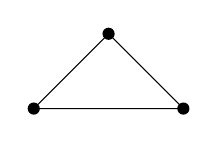
\begin{tikzpicture}[baseline=(b.base)]
\node (b) at (0.95,0.3) {};
\draw (0,0) -- (1.9,0) -- (0.95,0.95) -- cycle;
\fill (0,0) circle (2.2pt);
\fill (1.9,0) circle (2.2pt);
\fill (0.95,0.95) circle (2.2pt);
\end{tikzpicture}
\qquad\qquad\qquad ou \qquad\qquad\qquad
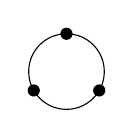
\begin{tikzpicture}[baseline=(c.base)]
\node (c) at (0,-0.1) {};
\draw (0,0) circle (0.48);
\fill (90:0.48) circle (2.2pt);
\fill (210:0.48) circle (2.2pt);
\fill (330:0.48) circle (2.2pt);
\end{tikzpicture}
\qquad\quad ,
\end{center}

subdivision barycentrique
\printedpage{48}
% head: A. Grothendieck : Dérivateurs, Ch. XVI, Édition des Universités de Montpellier II et Paris VII
% foot: Version 18 mars 2019

\begin{center}
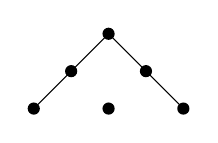
\begin{tikzpicture}[baseline=(b.base)]
\node (b) at (0.95,0.3) {};
\draw (0,0) -- (0.95,0.95) -- (1.9,0);
\fill (0,0) circle (2.2pt);
\fill (0.95,0) circle (2.2pt);
\fill (1.9,0) circle (2.2pt);
\fill (0.475,0.475) circle (2.2pt);
\fill (1.425,0.475) circle (2.2pt);
\fill (0.95,0.95) circle (2.2pt);
\end{tikzpicture}
\qquad\qquad\qquad ou \qquad\qquad\qquad
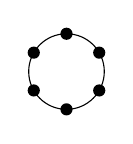
\begin{tikzpicture}[baseline=(c.base)]
\node (c) at (0,-0.1) {};
\draw (0,0) circle (0.48);
\fill (30:0.48) circle (2.2pt);
\fill (90:0.48) circle (2.2pt);
\fill (150:0.48) circle (2.2pt);
\fill (210:0.48) circle (2.2pt);
\fill (270:0.48) circle (2.2pt);
\fill (330:0.48) circle (2.2pt);
\end{tikzpicture}
\end{center}

(hexagone), que pour toute application croissante $g : I \longrightarrow \mathrm{sd}(I)$, sa réalisation topologique est homotope à une application constante, donc $g$ ne peut être un homotopisme dans Cat (car cela impliquerait que sa réalisation topologique est un homotopisme).

Ceci montre donc que la notion d'homotopisme dans Cat est \textit{strictement plus fine} que celle pour les réalisations topologiques, ce qui redonne à nouveau substance à l'espoir que l'invariant de Whitehead pourrait se définir comme invariant d'homotopie sur Cat, ou du moins sur une sous-catégorie pleine convenable, telle celle des ensembles ordonnés (éventuellement restreints à être finis), ou des maquettes simpliciales. Et même, que l'ensemble des Wh-types d'homotopie (types d'homotopie simples) peut se
\msp{page 96}
plonger canoniquement dans un $\mathrm{Hot}_W$ convenable, où $W$ serait un localiseur fondamental strictement plus fin que $\mathbf{W}_\infty$, p.ex. (qui sait ?) $\tilde{\mathbf{W}}_\infty$. Le premier travail qu'on aurait envie de faire, c'est de construire un tel $W$ \textit{ad hoc}, pour que l'invariant de Whitehead puisse s'écrire comme un foncteur sur $\mathrm{Hot}_{\bullet W}$. Pour commencer, il faudrait déjà s'assurer que cet invariant peut être vu comme un invariant du type d'homotopie, \textit{i.e.} qu'il s'interprète comme un foncteur sur $\mathrm{Hot}_{\bullet}\mathrm{Cat} \simeq \mathrm{Cat}(\,\underbrace{\text{homotop}}_{\substack{\text{ensemble des}\\ \text{homotopismes}}}\,)^{-1}$. Ce travail suggérera peut-être aussi la définition des “invariants de Whitehead supérieurs” (impliquant les $\pi_i$, non seulement le $\pi_1$), lesquels pourraient peut-être servir (avec celui de dimension 1) à décrire le localiseur hypothétique $W$ (“de Whitehead”).

\dgrblock{dgrb878}{A sharp degree bound for the polygon examples}
\begin{dcomment}{development}{p95}{A sharp degree bound for the polygon examples}
Grothendieck's six-point example is decisive because subdivision doubles the number of edges without giving a categorical homotopy inverse. We can make its obstruction quantitative, and thereby see that the phenomenon persists through every iterated subdivision.

For $m\geq3$, let $C_m$ be the height-one poset with minimal elements $v_i$ and maximal elements $e_i$, indexed by $i\in\mathbf Z/m$, and with the only strict relations
\[
 v_i<e_i,\qquad v_{i+1}<e_i.
\]
It is the face poset of a polygonal circle. Its order complex is a circle with $2m$ edges. A choice of the cyclic ordering fixes the sign of the degree of a map of realizations.

\textbf{Degree spectrum for crowns.}\ours\quad
For $m,n\geq3$, the degrees of the maps $|NC_m|\to|NC_n|$ induced by monotone maps $C_m\to C_n$ are exactly the integers $d$ satisfying $|d|n\leq m$.

\emph{Proof.} A monotone map induces a simplicial map of the order complexes. Each of the $2m$ domain edges maps either to a single target edge or to a vertex. Give every target edge length one, and lift the image of the oriented domain circle to the universal covering line of the target circle, starting at a chosen lift of its initial vertex. Each traversed domain edge changes the lifted coordinate by at most one in absolute value. After all $2m$ edges the displacement is $2nd$, where $d$ is the degree. Therefore $2n|d|\leq2m$.

For the converse, choose a closed walk of $m$ steps in the set of polygon vertices of the target. Its first $n|d|$ steps go around the polygon $|d|$ times, in the sign prescribed by $d$; all remaining steps are stationary at the initial vertex. Send the $i$th minimal element of $C_m$ to the $i$th vertex of this walk. If a step traverses a target edge, send the corresponding maximal element to that edge. If the step is stationary, send the maximal element to the same target vertex. In either case the images of both adjacent minimal elements are less than or equal to the image of the maximal element. This defines a monotone map. Its realized walk has degree $d$, as required.\hfill$\square$

The nonempty-chain poset $\operatorname{sd}(C_m)$ is isomorphic to $C_{2m}$: its minimal elements are the singleton chains, and its maximal elements are the two-element chains, arranged in the subdivided cycle. Induction gives $\operatorname{sd}^r(C_m)\cong C_{2^r m}$. For every $r\geq1$ the proposition forces every monotone map
\[
 C_m\longrightarrow\operatorname{sd}^r(C_m)
\]
to have degree zero. Maps between circles of degree zero are null-homotopic, whereas the maximum map in the other direction has degree one. No categorical homotopy inverse can exist. Taking $m=3$ and $r=1$ proves the claim on manuscript page~95 in full.

There is also a direct categorical rigidity check. If an endomap $h:C_m\to C_m$ satisfies $h\geq\id$, it fixes the maximal elements. The image of $v_i$ must then lie below both $e_{i-1}$ and $e_i$ and above $v_i$, forcing $h(v_i)=v_i$. Thus $h=\id$. Dually $h\leq\id$ also forces equality. Any finite zigzag of natural transformations starting at the identity is therefore constant. A categorical homotopy equivalence between two crowns would have strictly inverse composites and hence be an isomorphism; crowns of different sizes cannot be categorically homotopy equivalent.

The general distinction between finite-space homotopy and simple homotopy is established in the literature discussed next. We did not find this explicit degree-spectrum calculation in the consulted finite-space papers. We include it as an elementary development of Grothendieck's example, without a priority claim.
\end{dcomment}


\msp{page 97}

\dgrblock{dgrb879}{The finite-poset version of simple homotopy}
\begin{dcomment}{later}{p96}{The finite-poset version of simple homotopy}
Grothendieck's attempted localizer is ruled out by minimality, but his suggestion to work directly with finite ordered sets has a substantial later realization. These are two different claims, and the failure of the first does not diminish the second.

For a finite $T_0$ space, regarded as a finite poset, Barmak and Minian define elementary simplifications by deleting a weak point: a point whose strict lower set or strict upper set is contractible. Their Theorem~3.10 identifies the resulting simple-equivalence classes with simple homotopy types of finite simplicial complexes, through the order-complex and face-poset constructions. Their Theorem~4.13 gives the corresponding statement for maps \citep{BarmakMinian2008}. This is a precise version of the finite combinatorial program suggested here. It is not a fundamental localizer on all of $\Cat$ finer than $\mathbf W_\infty$.

The crown calculation explains why strict categorical homotopy equivalence is too fine for the desired comparison. A polygon and its subdivision have the same simple homotopy type, while their face posets have different strict categorical homotopy types. The elementary finite-space operations therefore must allow more than deletion of a point with a genuine order-theoretic deformation retraction. Conversely, passing all the way to weak homotopy equivalence forgets the simple structure. The successful theory sits between these two equivalence relations on finite models.

The invariant mentioned on manuscript page~88 also needs its classical input. For a homotopy equivalence $f:K\to L$ of connected finite CW complexes, Whitehead torsion is an element
\[
 \tau(f)\in\operatorname{Wh}(\pi_1L)
 =K_1(\mathbf Z[\pi_1L])/\langle\pm g\mid g\in\pi_1L\rangle.
\]
It vanishes exactly when the equivalence is simple, with the usual finite CW structures. It is attached to an equivalence and its simple structures, rather than being a canonical element attached to an unmarked homotopy type \citep[Section~7]{Milnor1966Whitehead}. Thus a proposed functorial invariant must specify its objects and morphisms before one asks whether it factors through a localization. The manuscript's suggestion of higher invariants does not specify enough data to identify it with a particular later torsion theory.

The page marked~94 is explicitly missing in the edition. The surrounding argument still supplies the finite counterexample and its purpose; we do not reconstruct an absent manuscript page from those conclusions.
\end{dcomment}


\section*{7\quad Commentaires sur les axiomes}

7.1. La principale raison d'être d'un localiseur fondamental $W$, c'est de définir une théorie d'homotopie’, et plus précisément un prédérivateur $\mathrm{HOT}_W$, dont on espère que ce sera même un dérivateur, ou qu'il satisfasse du moins à certains des axiomes des dérivateurs. Les axiomes Loc (1) à Loc (9) sont en majeure partie orientés vers cet objectif, à cela près que Loc (1, 2, 3) constitue un “minimum vital” absolu, pour pouvoir commencer à travailler avec $W$. Les principales questions qui se posent me paraissent les suivantes : % [sic] d'homotopie’ -> d'homotopie (or “théorie d'homotopie”), closing quote without opening quote
\begin{enumerate}[label={}, leftmargin=2.5em]
\item[1)] Quand Cat munie de $(W, \mathrm{Cof}_W)$, resp. de $(W, \mathrm{Fib}_W)$, est-elle une catégorie à cofibrations resp. à fibrations, de façon que les résultats de K. S. \textsc{Brown} soient applicables ?
\item[2)] Sous quelles conditions, sur $W$ et sur $f$, $f_!$ et $f_*$ existent-ils ? Et quand a-t-on, de plus, exactitude des carrés cocartésiens resp. cartésiens ?

\msp{page 98}
\item[3)] Plus généralement, en termes des axiomes imposés à $W$, quelles sont les axiomes Der (\ldots) que sont vérifiés pour le prédérivateur $\mathrm{HOT}_W$ ? (Ce qui pourrait aussi dépendre du choix du domaine Diag $\subset$ Cat. Le prédérivateur est défini a priori sur Cat tout entier). En particulier, % [sic] quelles sont les axiomes -> quels sont les axiomes, agreement; [sic] que sont vérifiés -> qui sont vérifiés, relative pronoun
\end{enumerate}

% ---- from der-ch16_p051-055.tex
\printedpage{49}
% head: A. Grothendieck : Dérivateurs, Ch. XVI, Édition des Universités de Montpellier II et Paris VII
% foot: Version 18 mars 2019

\begin{enumerate}[label=4)]
\item quand $\mathrm{HOT}_W$ est-il bel et bien un dérivateur sur Cat tout entier, \textit{i.e.} quand satisfait-il à tous les axiomes ?
\end{enumerate}

Une question qui me paraît moins importante (notamment que 1°) est la suivante :

\begin{enumerate}[label=1 bis)]
\item Quand $W$ s'insère-t-il dans un triple de Quillen clos $(W,C,F)$ (propre de préférence).
\end{enumerate}

Je vais passer en revue ces questions une à une.

7.2. On a vu (mais sans que j'aie fait une vérification soigneuse pour la réciproque) que $(W,\mathrm{Cof}_W)$ définit une structure à cofibrations si l'axiome \textit{Loc (6 a)} est satisfait, et que cette condition est aussi nécessaire si Loc (3 bis) est satisfait\footnote[45]{Vérifier quand même si Loc (3 bis) n'est pas déjà utilisé dans la partie directe ! \textbf{O.K.}}.

\msp{page 99}
Alors les immersions ouvertes de Dwyer (ou au choix les immersions fermées de Dwyer) sont dans $\mathrm{Cof}_W$, et la construction standard du mapping-cone définit, pour toute flèche $f$ dans Cat, une factorisation \textit{fonctorielle}
\[
\begin{aligned}
f = pi \quad & i \text{ immersion ouverte de Dwyer (donc dans } \mathrm{Cof}_W\text{),}\\
& p \in W.
\end{aligned}
\]
Cela, plus la construction du foncteur $f_!$, et en particulier des $W$-sommes amalgamées
\begin{tikzcd}[row sep=tiny, column sep=small, baseline=(\tikzcdmatrixname-2-1.base)]
 & X_1 \\
\displaystyle\int X_0 \arrow[ur] \arrow[dr] & \\
 & X_2
\end{tikzcd}, données dans VI (théorie de $\mathrm{HOT}_W$) et XII, nous donne une maîtrise parfaite (il me semble) sur la “structure homotopique gauche” définie par $W$, sous le seul axiome Loc (6 a) (Axiome du cube, forme directe). Je rappelle que les foncteurs $f_!$ sont construits dans VI sous la seule hypothèse \textit{Loc (3 bis)} ($f$ flèche quelconque de Cat), mais sauf erreur, la construction
\msp{page 100}
et l'interprétation $W$-homotopique de
\begin{tikzcd}[row sep=tiny, column sep=small, baseline=(\tikzcdmatrixname-2-1.base)]
 & X_1 \\
\displaystyle\int X_0 \arrow[ur] \arrow[dr] & \\
 & X_2
\end{tikzcd}
donnée dans XII ne dépend pas même de cette hypothèse\footnote[46]{\textit{cf.} XII, page 264} - mais je ne peux le garantir. Il me semble que XII (et notamment le long §5 sur les sommes amalgamées) est écrit sous l'hypothèse que W (1, 2, 3), \textit{i.e.} Loc (1, 2, 3bis), sont satisfaits.

7.3. C'est une chose assez extraordinaire que les foncteurs $f_!$ pour $\mathrm{HOT}_W$ existent, sous la seule hypothèse \textit{Loc (3 bis)} (axiome de localisation, forme forte) - et ils se “calculent” d'une façon féeriquement simple ! Je suis à peu près sûr que sous cette seule hypothèse, \textit{l'axiome d'exactitude pour les carrés cocartésiens} n'est \textit{pas} satisfait\footnote[47]{Il faudrait un exemple !}. Je ne vois aucun moyen de le vérifier, sauf via la théorie de \textsc{Brown}, sous l'hypothèse \textit{Loc (6 a)} (\textit{cf.} 7.2).

Mais sous la seule condition Loc (3 bis) le calcul standard des fibres d'un $f_!(\xi)$
\printedpage{50}
% head: A. Grothendieck : Dérivateurs, Ch. XVI, Édition des Universités de Montpellier II et Paris VII
% foot: Version 18 mars 2019
\msp{page 101}
est valable, en d'autre termes le prédérivateur $\mathrm{HOT}_W$ satisfait Der (4$^*$, 5$^*$) - et de plus Der (6$^*$) (exactitude “à gauche”) si $W$ satisfait Loc (6 a). % [sic] d'autre termes -> d'autres termes, missing plural s

7.4. Venons-en à la question si Cat muni de $(W,\mathrm{Fib}_W)$ est une catégorie à fibrations. C'est l'axiome \textit{Loc (7 F),} mais je ne connais guère de moyen de le vérifier (en dehors du cas très, très particulier $W = \mathbf{W}_0$) que moyennant tout au moins l'axiome \textit{Loc (7 $D_{W_\omega}$),} ou l'une ou l'autre des variantes plus fortes de Loc (7). De Loc (7 $\mathrm{D}_{W_\omega}$) il a été abondamment question précédemment, \textit{cf.} notamment 6.4 (pages 89-91). En mon sens, cet axiome assure une maîtrise comparable sur la structure $W$-homotopique droite (fibres $W$-homotopiques, suites exactes de cosuspension) que Loc (6 a) pour la
\msp{page 102}
structure gauche. En particulier, on a la factorisation \textit{fonctorielle} de toute flèche $f$ de Cat en
\[
f = pi, \qquad i \in W_\omega \subset W,\ p \in \mathrm{Parf}_{W_\omega} \subset \mathrm{Fib}_W .
\]
Mais \textit{l'axiome Loc (7 $D_{W_\omega}$) me paraît de nature considérablement plus forte que Loc (6 a),} lequel (si je ne m'abuse) est vérifié pour tous les localiseurs qui ont été envisagés jusqu'à présent. (Mais j'avoue n'avoir pas regardé le cas des $\mathbf{W}_n$, $n \in \mathbf{N}$, sauf $\mathbf{W}_0$.) Par contre, l'axiome Loc (7 $\mathrm{D}_{W_\omega}$) implique $W \subset \mathbf{W}_\infty$ (théorème 6.1), relation vraiment draconienne (\textit{cf.} commentaire 6.4 a).

Par ailleurs, le seul axiome Loc (7 $\mathrm{D}_{W_\omega}$), pour autant que je sache, n'implique pas l'existence de $f_*$ pour \textit{toute} flèche dans Cat, mais seulement pour des
\msp{page 103}
flèches de la forme $f \times \mathrm{id}_X : S \times X \longrightarrow T \times X$, où $f : S \longrightarrow T$ est un morphisme entre ensembles ordonnés finis. Ou plus généralement, entre ensembles ordonnés $S$, $T$ tels que $S^\circ$ soit artinien, \textit{i.e.} $\mathrm{S}$ noethérien, et que $\mathrm{Esp}(S^\circ)$ soit noethérien (cette dernière hypothèse étant inutile sous l'axiome Loc (8) des limites, \textit{cf.} XVII, th. 3.1, p. 50). Donc ce n'est pas le résultat rêvé.

7.5. Le seul cas que je connaisse où $f_*$ existe pour \textit{toute} flèche dans Cat, est le cas où $W$ satisfait à
\[
\textit{Loc (6 a, 8, 9)}\ \ \text{\footnotemark[48]\,\footnotemark[49]}, \tag*{$(*)$} % [sic] marks printed (48) (49) -> the two footnotes printed below are numbered 49 and 50, numbering mismatch between marks and footnotes
\]
\footnotetext[49]{Vérifier s'il ne faut pas aussi la condition Loc (3 bis) en plus de Loc (6 a, 8, 9). Vérification faite, c'est O.K. (sans Loc (3 bis)).}
\footnotetext[50]{\textbf{N.B.} Après nouvelle réflexion, il apparaît qu'il suffit même Loc (6$'$ a, 8, 9).}
c'est à dire l'axiome des $W$-cofibrations faibles, déjà abondamment mentionné et enfin ceux des limites et d'accessibilité, \textit{i.e.} $W$ est $\mathrm{L}_1$-accessible dans \underline{Fl}(Cat). Le résultat-clef pertinent est donné dans XV 8.4 (p. 105-107), qu'il faut joindre à XV 7.4 (p. 98-99) pour en faire
\msp{page 104}
bon usage, et en déduire le théorème 10.1 (XV, p. 134-135). Mieux que l'existence des $f_*$, l'ensemble d'axiomes étonnamment faible que je viens d'expliciter suffit à assurer que $\mathrm{HOT}_W$ est un \textit{dérivateur} sur Cat tout entier, en plein sens du terme, \textit{i.e.} qu'il satisfait à Der (1, 2, 3, 4, 5, 6, 4$^*$, 5$^*$, 6$^*$). Ceci est obtenu en remplaçant (grâce à XV 8.4) Cat par
\printedpage{51}
% head: A. Grothendieck : Dérivateurs, Ch. XVI, Édition des Universités de Montpellier II et Paris VII
% foot: Version 18 mars 2019
$A^\wedge$, où $A$ est une catégorie-test convenable, $W$ par $W_A \subset \mathrm{Fl}\, A^\wedge$, et en prouvant que $W_A$ s'insère dans un triple de Quillen clos $(W,C,F)$, avec $C = \mathrm{Mono}(A^\wedge)$, ce qui détermine $F$ comme $(C \cap W_A)_*$. On applique alors XV 7.4 à cette situation (résultats résumés dans XIX, th. 2.3 (p. 19), 2.6 (p. 25), 2.9 (p. 28). On retrouve l'existence des $f_!$ (avec un mode de calcul bien différent de celui dans Cat !), et en plus on trouve l'existence de $f_*$ (plus l'exactitude dans cor. [?] 5
\msp{page 105}
des carrés $W$-cartésiens) - ce qui pour moi, pendant un bon moment, était \textit{le} gros problème pour la théorie de $\mathrm{HOT}_W$ !).

\dgrblock{dgrb880}{A presentation supplies operations at every diagram shape}
\begin{dcomment}{exposition}{p104}{A presentation supplies operations at every diagram shape}
The shift from $\Cat$ to a presheaf category is a change of computational model. Its purpose is to make the homotopy theory of diagrams available uniformly. A homotopy category alone contains too little information for this task: an object of $\operatorname{Ho}(\mathcal M)^S$ is a diagram whose relations commute only after localization, whereas an object of $\operatorname{Ho}(\mathcal M^S)$ retains a coherent realization of those relations. A derivator keeps the latter categories, their restrictions, and their homotopy Kan extensions. This distinction is why the existence of $f_*$ for every shape is stronger than the ability to write down a fibre for a single arrow.

Modern statements require some translation before they can be applied here. In \citet[Definition~1.5]{Groth2013}, Der~(1) concerns arbitrary small coproducts of shapes, Der~(2) says that evaluations jointly detect isomorphisms, Der~(3) gives both Kan adjoints, and Der~(4) calculates them pointwise. Grothendieck's original numbering separates the existence, calculation, and exactness assertions into Der~(4)--(6) and their starred partners; his Der~(3) is a contractibility condition. Moreover, the convention here uses presheaves $\mathcal M(S)=\mathcal M^{S^{\rm op}}$. Passing to opposite shapes translates this convention into the covariant diagrams used by many modern authors. Numbers and the words ``left'' and ``right'' cannot safely be transferred without that translation.

For a combinatorial model category the modern realization theorem is \citet[Proposition~1.30]{Groth2013}. The proof uses diagram model structures to derive restriction and ordinary Kan extension. It supplies the uniform operations sought in these pages. A complementary comparison is \citet[Theorem~3.33]{Lenz2018}: the homotopy prederivator of a cofibration category agrees with that of its quasicategory of frames. Its Corollary~4.1 then obtains the corresponding derivators from complete or cocomplete quasicategories. These are precise realization and comparison results. They do not say that every prederivator is representable by a model category, or that the original class $W$ can automatically be recovered from any equivalent presentation. The latter is a separate recognition argument, undertaken on manuscript pages~111--118.
\end{dcomment}


Je trouve époustouflant qu'on parvienne à un résultat aussi fort avec des axiomes aussi ridiculement faibles. Plus particulièrement, qu'on ait toutes les propriétés désirables de la structure homotopique droite, sans avoir à faire sur $W$ aucune hypothèse du type $W$-fibration ! Ces axiomes n'impliquent \textit{pas} l'axiome Loc (7) (équivalent à Loc (7 $\mathrm{D}_{W_\omega}$) en présence de Loc (8)), comme on a vu sur l'exemple de $\mathbf{W}_0$. Impliquent-ils tout au moins Loc (7 F), \textit{i.e.} l'existence d'assez de $W$-fibrations ? Je ne hasarderais aucune conjecture à ce sujet ! Mais il faut bien se dire qu'en l'absence de Loc (7) (et même
\msp{page 106}
en admettant Loc (7 F)), tout en sachant que la structure homotopique droite associée à $W$ est parfaite à tous égards, on n'a a priori aucune maîtrise sur celle-ci, notamment pour le calcul des fibres $W$-homotopiques et la construction des carrés $W$-cartésiens. Même en ramenant toutes ces constructions à $A^\wedge$ (prenant, si on y tient, $A = \boldsymbol{\Delta}$, \textit{i.e.} se ramenant au contexte semisimplicial), quoi qu'on sache qu'il y a une factorisation \textit{fonctorielle} $f = pi$ avec $i \in \mathrm{TC} \subset W_A$, $p \in F \subset \mathrm{Fib}_{W_A}$, je ne vois aucune façon concrète de l'expliciter. À moins que la considération des chemins infinis, qui (en l'absence de Loc (7)) s'avère inopérante dans Cat sauve la mise dans $\boldsymbol{\Delta}^\wedge$ ? ?

\msp{page 107}
Question qui devrait être facile à élucider, mais sur laquelle je ne veux pas m'attarder à présent.

Notons en passant que le résultat de saturation forte de \textsc{Quillen}, pour les triples de Quillen clos, montre que l'ensemble d'axiomes $(*)$ implique l'axiome Loc (1 ter), \textit{i.e.} que $W$ est \textit{fortement saturé.}

Notons aussi que contrairement à ce qui a lieu pour les $f_!$, je ne sais prouver l'existence de $f_*$, et notamment des suites de cosuspension, que sous des conditions (soit Loc (7 $\mathrm{D}_{W_\omega}$), soit Loc (6a, 8, 9)) qui assurent déjà que les carrés $W$-cartésiens sont exacts, et par suite les suites de cosuspension exactes.

Je pense que dans les pages précédentes, j'ai dit tout ce que je sais dire de pertinent, concernant les questions 1, 2, 4 soulevées dans 7.1. Ces réponses me parais\msp{page 108}sent satisfaisantes - plus satisfaisantes que je ne l'aurais osé espérer pendant les premiers deux mois de mes cogitations ! Il reste les questions 3 et 1 bis, que je vais à présent examiner.

\printedpage{52}
% head: A. Grothendieck : Dérivateurs, Ch. XVI, Édition des Universités de Montpellier II et Paris VII
% foot: Version 18 mars 2019
7.6. Sur les différents axiomes des dérivateurs : sous quelles conditions sur $W$ un de ces axiomes est-il satisfait pour $\mathrm{HOT}_W$\footnote[51]{Pour les axiomes Der (1) à Der (5$^*$), \textit{cf.} I, p. 67-68. Les axiomes Der (6, 6$^*$) sont les axiomes d'exactitude, dont la nécessité m'est apparue seulement ultérieurement.} ? Pour ce qui est des axiomes Der (4, 5, 6, 4$^*$, 5$^*$, 6$^*$), je crois avoir dit tout ce que je sais en dire, et avoir des critères ce validité parfaitement maniables, dans les pages précédentes. Résumons pourtant : % [sic] ce validité -> de validité, misprint
\[
\left\{
\begin{array}{lcl}
\text{structure à cofibrations} & : & \text{Loc (6) (+ Loc (3 bis) ?)} \\[1ex]
\text{structure à fibrations} & : & \text{Loc (7 }\mathrm{D}_{W_\omega}\text{)} \\[1ex]
\text{Der (4}^*\text{, 5}^*\text{)} & : & \text{Loc (3 bis)} \\[1ex]
\text{Der (4}^*\text{, 5}^*\text{, 6}^*\text{)} & : & \text{Loc (3 bis, 6a) ou Loc (6}'\text{ a, 8, 9)} \\[1ex]
\text{Der (4, 5, 6) (sur Cat) (et tout le reste !)} & : & \text{Loc (6}'\text{ a, 8, 9)} \\[1ex]
\text{Der (4, 5, 6) (sur Diag $=$ ens. ordonnés finis)} & : & \text{Loc (7 }\mathrm{D}_{W_\omega}\text{) (ou seulement Loc (7 F)).}
\end{array}
\right.
\]

Il reste les axiomes Der (1) (décomposition), Der (2) (localisation), Der (3) (objet unité), que je vais passer à présent en revue. On vérifie
\msp{page 109}
de façon quasi-tautologique que l'axiome Der 1 est satisfait sans condition sur $W$ (pas même Loc (2, 3) !) - en fait, il est satisfait pour tout prédérivateur $\mathbf{D}_{(\mathcal{M},W)}$ défini par une catégorie de modèles.

L'axiome de localisation Der (2) est par contre de nature délicate. Il est valable, plus généralement, pour une catégorie de modèles $(\mathcal{M},W)$ (définissant un prédérivateur $\mathbf{D} = \mathbf{D}_{(\mathcal{M},W)}$) et un objet $S$ de Cat, lorsque $(\mathcal{M}(S),W(S))$ est associé à une structure à fibrations ou à cofibrations, ce qui par K. S. \textsc{Brown} implique que toute flèche de $\mathrm{HO}_W(S) = \mathcal{M}(S)W(S)^{-1}$ se “réalise” par une flèche de $\mathcal{M}(S)$ - et alors le résultat est évident. La condition que je viens de dire est satisfaite lorsque $(\mathcal{M},W)$ lui-même est associé à une structure de cofibrations ou de fibrations,
\msp{page 110}
et si de plus on suppose que l'on est dans l'un de deux cas suivants : % [sic] l'un de deux cas -> l'un des deux cas, apparent misprint
\begin{enumerate}[label=\alph*)]
\item $S$ est un ensemble ordonné fini (ce qui nous amène à nous restreindre, à défaut de mieux, à Diag $=$ sous-catégorie de Cat formée des ensembles ordonnés finis).
\item La factorisation stipulée dans l'axiome de factorisation $f = pi$ (avec $i \in \mathrm{Cof}$, $p \in W$ (cas de cofibrations) ou $i \in W$, $p \in \mathrm{Fib}$ (cas de fibrations)) peut être choisie fonctorielle en $f$.
\end{enumerate}
Or, dans le cas de Cat, dans les cas où on sait prouver que $W$ est associé à une structure à cofibrations (axiome \textit{Loc (6 a)}) où à fibrations (axiome \textit{Loc (7 $D_{W_\omega}$)}), on trouve bel et bien une factorisation fonctorielle. Donc chacun de ces axiomes implique Der (2). % [sic] où à fibrations -> ou à fibrations, accent misprint

\dgrblock{dgrb881}{Finite coproducts of shapes and the length of a zigzag}
\begin{dcomment}{examples}{p109}{Finite coproducts of shapes and the length of a zigzag}
The assertion called quasi-tautological is correct in its original scope. Chapter~I, manuscript page~67, footnote~3, defines Der~(1) for a \emph{finite} sum of shapes. Let $(\mathcal C,U)$ and $(\mathcal E,V)$ be relative categories, with identities among their weak equivalences. There is a canonical equivalence
\[
 (\mathcal C\times\mathcal E)[(U\times V)^{-1}]
 \simeq \mathcal C[U^{-1}]\times\mathcal E[V^{-1}].
\]
Here is the mechanism. Every ordinary arrow $(a,b)$ factors as $(a,1)$ followed by $(1,b)$. A formal inverse of $(u,v)$ decomposes in the same fashion, using the inverses of $(u,1)$ and $(1,v)$. Horizontal and vertical arrows commute in every rectangle. The same commutation holds when one or both arrows are inverted, by multiplying the commutative square by the relevant inverses. Thus a word in the localized product can be rearranged into a word in the first coordinate followed by a word in the second. Conversely, two localized coordinate words define such a composite; the defining composition, identity, and inverse relations in either coordinate remain valid in the product localization. These operations are mutually inverse on hom-sets and preserve composition. This proves the equivalence, including its faithfulness.

Induction gives finite products. Since
\[
 \mathcal M^{(S\amalg T)^{\rm op}}
 \cong \mathcal M^{S^{\rm op}}\times\mathcal M^{T^{\rm op}},
\]
and objectwise weak equivalences correspond under this isomorphism, localizing proves finite Der~(1). The empty shape gives the terminal category as well. No localizer axiom is needed.

An explicit example explains why the same reasoning must not be extended to infinitely many factors without hypotheses. For $n\geq1$, let $J_n$ have objects $0,\ldots,n$, with precisely the nonidentity arrows between adjacent vertices directed from the even vertex to the odd vertex. Thus every nonidentity arrow has length one, and no two nonidentity arrows compose. Let $\mathcal M=\coprod_{n\geq1}J_n$ and declare every arrow a weak equivalence. In $\mathcal M^{\mathbb N}$ take objects $x$ and $y$ whose $n$th coordinates are the vertices $0$ and $n$ in $J_n$. Each coordinate has a finite zigzag joining these vertices, so their images are isomorphic in $\prod_n\operatorname{Ho}(\mathcal M)$.

There is nevertheless no arrow from $x$ to $y$ in $\operatorname{Ho}(\mathcal M^{\mathbb N})$. Such an arrow would be represented by a finite word of, say, $k$ ordinary arrows and formal inverses. In coordinate $n$, each letter changes the vertex by at most one. Hence the word can travel at most $k$ edges, whereas the endpoints in $J_n$ are $n$ edges apart. Taking $n>k$ gives a contradiction. The comparison to the infinite product is therefore not full. The obstruction is the absence of a uniform finite zigzag, not a defect in Grothendieck's finite axiom. Modern arbitrary-coproduct Der~(1) requires the additional homotopical structure supplied by the realization theorems. A related bounded-length obstruction already occurs in \citet[p.~307]{Thomason1980}, where the fundamental group of an infinite product of elementary categorical circles gives bounded integer families rather than all integer families.
\end{dcomment}


\msp{page 111}
Reste l'axiome de contractibilité : si $S$ dans Cat est contractile, est-il $\mathrm{HOT}_W$-asphérique, \textit{i.e.} le foncteur
\[
\mathrm{HOT}_W(e) = \mathrm{Hot}_W \longrightarrow \mathrm{HOT}_W(S)
\]
\printedpage{53}
% head: A. Grothendieck : Dérivateurs, Ch. XVI, Édition des Universités de Montpellier II et Paris VII
% foot: Version 18 mars 2019
est-il pleinement fidèle ? Quand on dispose de la théorie de $f_!$ “version Cat” (donc sous le seul axiome \textit{Loc (3 bis)}), on trouve ceci (noté dans VI, p. 202)\footnote[52]{moyennant Loc (3 bis).} :
\begin{quote}
Soit $f : S \longrightarrow T$ une flèche dans Cat. Pour que ce soit une $\mathrm{HOT}_W$-équivalence, \textit{i.e.} pour que $f^* : \mathrm{HOT}_W(T) \longrightarrow \mathrm{HOT}_W(S)$ induise un foncteur \textit{pleinement fidèle} sur la sous-catégorie des objets constants de $\mathrm{HOT}_W(T)$, il faut et il suffit que $\mathrm{hot}_W(f) : \mathrm{hot}_W(S) \longrightarrow \mathrm{hot}_W(T)$ soit un isomorphisme. Donc il \textit{suffit} que $f \in W$, et cette condition est aussi nécessaire si $W$ est fortement saturé (axiome Loc (1 ter)).
\end{quote}
Par acquit de conscience, j'explicite ici la démonstration. L'existence des foncteurs
\msp{page 112}
$f_!$, en particulier des objets d'homologie $H_\bullet^{\mathrm{HOT}_W}(S,\xi)$ (où simplement $H_\bullet^W(S,\xi)$) pour $\xi \in \mathrm{HOT}_W(e) = \mathrm{Hot}_W$, permet d'interpréter homologiquement la condition de $\mathrm{HOT}_W$-équivalence, comme signifiant que pour tout $\xi = \mathrm{hot}_W(X)$ dans $\mathrm{Hot}_W$, la flèche canonique dans $\mathrm{Hot}_W$ % [sic] (où simplement -> (ou simplement, accent misprint
\[
H_\bullet^W(S,\xi) \longrightarrow H_\bullet^W(T,\xi) \tag*{$(*)$}
\]
est un isomorphisme. Or le calcul des $f_!$ (dans le cas de $p : S \longrightarrow e$ et de $T \longrightarrow e$) nous montre que les deux membres de $(*)$ ne sont autres (à isomorphisme près) que $\mathrm{hot}_W(X \times S)$ et $\mathrm{hot}_W(X \times T)$, la flèche étant induite par
\[
\mathrm{id}_X \times f : X \times S \longrightarrow X \times T. \tag*{$(*)$}
\]
Donc la condition envisagée signifie que cette flèche est un isomorphisme dans $\mathrm{Hot}_W$ pour tout $X$ dans Cat. Prenant $X = e$, on voit que cela implique que $\mathrm{hot}_W(f)$ est un isomorphisme, et cela suffit, vu que le
\msp{page 113}
foncteur $\mathrm{hot}_W : \mathrm{Cat} \longrightarrow \mathrm{Hot}_W$ commute aux produits finis (il suffit de Loc (1, 2, 3)) \texttt{[plutôt Loc (1, 2, 3 bis)]} et que la flèche $(*)$ dans $\mathrm{Hot}_W$ s'identifie à
\[
\mathrm{id}_{\mathrm{hot}_W(X)} \times \mathrm{hot}_W(f)\,.
\]
Cela montre donc que si $S$ est un objet $W$-asphérique, \textit{i.e.} tel que $S \longrightarrow e$ soit dans $W$ (et a fortiori, si $S$ est contractile), alors $S \longrightarrow e$ est $\mathrm{HOT}_W$-asphérique.

\dgrblock{dgrb882}{What it means to realize a localized arrow}
\begin{dcomment}{exposition}{p110}{What it means to realize a localized arrow}
The word ``realize'' in the proof of Der~(2) permits replacement of the source and target by weakly equivalent objects. It does not say that the localization functor is full on the original, fixed pair of objects. Even a formal inverse of a weak equivalence need not be represented by an ordinary arrow in the reverse direction between those same objects.

In a model category, the precise calculation uses a cofibrant replacement $QX\to X$ and a fibrant replacement $Y\to RY$. Every arrow $X\to Y$ in the homotopy category is represented by an ordinary map $QX\to RY$. Applied in a suitable diagram model category, this gives a map of replacement diagrams. If every component of the original localized arrow is an isomorphism, every component of the representing map is an isomorphism in the base homotopy category. Strong saturation of model weak equivalences makes those components weak equivalences. The representing map is therefore an objectwise weak equivalence, and becomes an isomorphism in the localized diagram category. The weak-equivalence replacements show that the original arrow is also invertible. This proves the pointwise conservativity required by Der~(2).

Grothendieck invokes the analogous Brown calculation for a cofibration or fibration category. In the finite-poset case, one constructs the necessary replacement diagram inductively, placing an object after its already treated predecessors and factoring the resulting latching map, or dually using matching maps. A functorial factorization can instead be applied directly to natural transformations; functoriality makes the chosen middle objects into a diagram. This is the specific advantage of the functorial constructions recalled on pages~99 and~102.

For all small shapes, a modern cofibration-category theorem carries more structure than a finite Brown theorem. \citet[Definition~1.5 and Warning~1.7]{Lenz2018} explicitly includes coproduct and sequential-colimit conditions in the ABC framework. The distinction matters: a proof that works by finite induction cannot simply be reindexed by an arbitrary small category. Conversely, a theorem proved for ABC cofibration categories should not be used to certify an unqualified claim about every finite Brown category. Lenz's Example~1.49 also exhibits a general relative category whose homotopy prederivator fails even weak strength. A class of denominators alone supplies a prederivator; the homotopical factorization and gluing conditions do substantive work.
\end{dcomment}


Pour résumer, on trouve le tableau
\[
\left\{
\begin{array}{lcl}
\text{Der (1)} & : & \text{sans hypothèse sur } W \\[1ex]
\text{Der (2)} & : & \text{Loc (6 a) \textit{ou} Loc (7 }\mathrm{D}_{W_\omega}\text{)} \\[1ex]
\text{Der (3)} & : & \text{Loc (3 bis) \textit{ou} Loc (6}'\text{ a, 8, 9)\ \ \footnotemark[53].}
\end{array}
\right.
\]
\footnotetext[53]{\textbf{N.B.} On verra plus bas que Loc (6 a, 8, 9) implique déjà Loc (3 bis).}

7.7. Il faut seulement justifier encore que Loc (6$'$ a, 8, 9) implique Der (3). Mais alors, on l'a vu, $\mathrm{HOT}_W$ peut être défini par un triple de Quillen très spécial. Mais même pour un triple de Quillen spécial sans plus $(\mathcal{M},W)$, le prédérivateur $\mathbf{D}$ qu'il définit satisfait (en plus de Der (4$^*$, 5$^*$, 6$^*$)) aux conditions Der (1) (trivialement), Der (2)

% ---- from der-ch16_p056-059.tex
\printedpage{54}
% head: A. Grothendieck : Dérivateurs, Ch. XVI, Édition des Universités de Montpellier II et Paris VII
\msp{page 114}
(\textit{cf.} p. 110, cas b)) et \textit{de plus} Der (3). (Donc dans le cas d'un triple de Quillen \textit{très} spécial, le prédérivateur obtenu est bel et bien un dérivateur.) Je vais expliciter ici la démonstration.

\dgrblock{dgrb883}{Recovering the equivalences from constant diagrams}
\begin{dcomment}{exposition}{p113}{Recovering the equivalences from constant diagrams}
The recognition calculation is a particularly useful part of this survey. It also records exactly where the later circular argument will enter. Let $\mathbb D=\mathrm{HOT}_W$, let $p_S:S\to e$, and write $c_S=p_S^*$. Assuming the left Kan extensions constructed under Loc~(3~bis), set
\[
 H(S,\xi)=p_{S!}c_S\xi.
\]
Adjunction identifies
\[
 \operatorname{Hom}_{\mathbb D(S)}(c_S\xi,c_S\eta)
 \cong
 \operatorname{Hom}_{\mathbb D(e)}(H(S,\xi),\eta).
\]
For $f:S\to T$, restriction on constant objects corresponds under this identification to precomposition with the canonical map
\[
 H(S,\xi)\longrightarrow H(T,\xi).
\]
Consequently restriction is fully faithful on constants precisely when these maps are isomorphisms for every $\xi$. For the nontrivial direction, bijectivity of the displayed hom-set maps for every $\eta$ implies the assertion by the ordinary Yoneda criterion for an isomorphism. This is the exact reason that a condition on all morphisms between constants can be tested by homology objects.

Write $q:\Cat\to\mathrm{Hot}_W$ for localization. Every object $\xi$ of this homotopy category is represented by a category $X$. The categorical Kan-extension calculation gives
\[
 H(S,qX)\cong q(X\times S),\qquad
 H(T,qX)\cong q(X\times T),
\]
with the comparison induced by $1_X\times f$. Taking $X=e$ shows that full faithfulness on constants forces $q(f)$ to be an isomorphism. Conversely, the product calculation identifies the comparison with $1_{qX}\times q(f)$, so invertibility of $q(f)$ implies all the required isomorphisms. The argument thus identifies the class of $\mathbb D$-equivalences with
\[
 \{f\mid q(f)\text{ is an isomorphism}\}.
\]
It identifies that class with $W$ itself only when $W$ is strongly saturated. This qualification is expressly present on page~111.

There are two different localization facts in this proof. The preceding block used finite products of \emph{categories being localized} to prove finite Der~(1). Here one needs the cartesian product operation on $\Cat$ to descend to its localization and to agree with the products used in the homology formula. That uses the localizer's stability properties and the preceding Kan-extension theory. Grothendieck's bracketed correction from Loc~(1,2,3) to Loc~(1,2,3~bis) is therefore retained in the audited reading; a formal finite-product localization lemma cannot remove the hypothesis from the whole recognition argument.

For $T=e$, a $W$-aspherical $S$ has $q(S)\cong e$, so the comparison is invertible for every $X$. Thus $c_S$ is fully faithful. This verifies the contractibility axiom in this setting without identifying a contractible diagram shape with an arbitrary diagram category: constant diagrams embed fully faithfully, while nonconstant diagrams can still contain substantial information.
\end{dcomment}


Je vais désigner par $(\mathcal{M},\Sigma)$ la catégorie de modèles donnée ($\Sigma\subset\operatorname{Fl}\mathcal{M}$), par $\mathbf{D}=\mathbf{D}_{\mathcal{M},W}$ le prédérivateur correspondant, et par
\[ W=W_D \] % [sic] W_D -> W_{\mathbf{D}}, index printed as italic D, elsewhere bold D
le localiseur dans Cat associé, formé des ``$\mathbf{D}$-équivalences''. On voit tout de suite que $W$ est fortement saturé (vrai pour tout $W_{\mathbf{D}}$, $\mathbf{D}$ un prédérivateur), \textit{i.e.} satisfait Loc (1 ter), a fortiori Loc (1), d'autre part il satisfait à Loc (3 bis$^*$), comme conséquence du fait que $\mathbf{D}$ satisfait à Loc (4$^*$, 5$^*$). A fortiori il satisfait à Loc (3$^*$), et pour voir que tout $X$ contractile dans Cat est $W$-asphérique, \textit{i.e.} $X\longrightarrow e$ dans $W$, on sait (\textit{cf.} §1)
\msp{page 115}
qu'il suffit de prouver qu'il en est ainsi si $X$ a un objet initial (axiome Loc (2$^*$) dual de l'axiome Loc (2)). À ce moment, on saura que $W$ est un localiseur fondamental, et de plus il satisfait Loc (3$^*$ bis), donc aussi Loc (3 bis) (forme forte de l'axiome de localisation).

Donc \textit{on peut supposer} que si $S$ a un objet initial, alors $S$ est $W$-asphérique, \textit{i.e.} $S\longrightarrow e$ est dans $W$, \textit{i.e.} $p^*:\mathbf{D}(e)\longrightarrow\mathbf{D}(S)$ est pleinement fidèle. Il revient au même de dire que la flèche d'adjonction
\[ p_!p^*\xi\longrightarrow\xi \]
est un isomorphisme, pour tout $\xi$ dans $\mathbf{D}(e)$. Or le calcul de $p_!(\eta)$ (pour $\eta\in\operatorname{Ob}\mathbf{D}(S)$, \textit{i.e.} $\eta\in\operatorname{Ob}\mathcal{M}(S)$) se fait ainsi : on choisit une flèche
\[ \eta'\xrightarrow{\Sigma_S}\eta \]
avec $\eta'$ ``cofibrant'' (pour la structure à cofibrations pertinente sur $\mathcal{M}(S)$), et on
\msp{page 116}
pose \footnote[54]{opération $p_!$ au niveau de $\mathcal{M}(S)$.}
\[ p_!(\operatorname{ho}_{W,S}(\eta))=\operatorname{ho}_W(p_!(\eta')). \]
Quand $\eta=p^*(\xi)$, la flèche d'adjonction pertinente dans $\operatorname{Ho}_\Sigma=\mathbf{D}(e)$ s'obtient par composition
\[ p_!(\eta')\longrightarrow p_!(p^*(\xi))\xrightarrow{\text{adj.}}\xi, \tag*{$(*)$} \]
où ici $p_!$ est encore pris dans le sens ordinaire ($\mathcal{M}(S)\longrightarrow\mathcal{M}(e)=\mathcal{M}$). Or $S$ ayant un objet initial 0, on a
\[ \begin{aligned}
p_!(\eta') &\ \simeq\ \eta'(0)\\
p_!(p^*(\xi)) &\ \simeq\ p^*(\xi)(0)\ \simeq\ \xi,
\end{aligned} \]
et la flèche d'adjonction dans $(*)$ est l'identité, la première flèche est la flèche $\eta'(0)\longrightarrow\eta(0)$ induite par $\eta'\longrightarrow\eta$, elle est dans $\Sigma$, donc $(*)$ est dans $\Sigma$, donc c'est un isomorphisme dans $\operatorname{Ho}_\Sigma=\mathbf{D}(e)$, q.e.d.

Le même argument marche d'ailleurs si $\mathcal{M}$ est seulement une catégorie à cofibrations ou à fibrations, mais en se bornant alors au cas où $S$ est un ensemble ordonné fini.
% foot: Version 18 mars 2019

% Original hard page break suppressed for the reflowed reader.
\printedpage{55}
% head: A. Grothendieck : Dérivateurs, Ch. XVI, Édition des Universités de Montpellier II et Paris VII
\msp{page 117}
Je vais dégager à part ce qu'on vient d'obtenir :

\dgrblock{dgrb884}{Why the initial object computes this left adjoint}
\begin{dcomment}{exposition}{p116}{Why the initial object computes this left adjoint}
There is no initial-versus-terminal mistake in the displayed calculation. Its direction records the presheaf convention. An object of $\mathcal M(S)$ is a functor $S^{\rm op}\to\mathcal M$. If $0$ is initial in $S$, it is terminal in $S^{\rm op}$, and hence
\[
 p_!\eta=\mathop{\rm colim}_{S^{\rm op}}\eta\cong\eta(0).
\]
For completeness, the cocone is given by the unique arrows $s\to0$ in $S^{\rm op}$. A cocone from $\eta$ to an object $z$ is uniquely determined by its component $\eta(0)\to z$, since compatibility forces every other component to be its composite with $\eta(s)\to\eta(0)$. This proves the universal property and the natural isomorphism.

Now take an object $\xi\in\mathcal M$, let $c\xi=p^*\xi$, and choose a cofibrant replacement of this diagram,
\[
 q:Q(c\xi)\longrightarrow c\xi,
\]
whose components belong to $\Sigma$. The derived counit of $\mathbf Lp_!\dashv p^*$ is represented by
\[
 p_!Q(c\xi)\longrightarrow p_!c\xi\longrightarrow\xi.
\]
Under the displayed evaluation isomorphisms this is simply $q_0:Q(c\xi)(0)\to\xi$, because the second arrow is the identity. It is a weak equivalence, so the derived counit is an isomorphism. A right adjoint is fully faithful exactly when its counit is an isomorphism. Therefore the constant-diagram functor is fully faithful, which is the required asphericity conclusion for this shape.

The argument proves a property of the derivator produced by the model structure. It has no need to identify its associated fundamental localizer with a previously given $W$. That is why Proposition~7.7.1 can be used to verify the original Der~(3) independently of the disputed recognition statement. The symbols $W$ and $\Sigma$ in the surrounding text should still be distinguished: $\Sigma$ denotes weak equivalences in the chosen model category, whereas $W_{\mathbb D}$ is a class of functors between small categories. Several printed subscripts switch them inadvertently; the correction ledger records those slips without rewriting the edition.
\end{dcomment}


\textbf{Proposition 7.7.1.} \textit{Soit} $(\mathcal{M},W)$ \textit{une catégorie de modèles, associée à un triple de Quillen clos} spécial $(W,C,F)$\textit{. Alors le prédérivateur} $\mathbf{D}=\mathbf{D}_{\mathcal{M},W}$ \textit{sur} Cat \textit{satisfait aux axiomes} Der (1, 2, 3, 4$^*$, 5$^*$, 6$^*$)\textit{. Si de plus le triple de Quillen est} très \textit{spécial} (\textit{donc en particulier} $C=\operatorname{Mono}(\mathcal{M})$), \textit{alors il satisfait de plus à} Der (4, 5, 6), i.e. \textit{c'est un dérivateur au plein sens du terme. D'autre part, le localiseur} $W=W_{\mathbf{D}}$ \textit{dans} Cat \textit{associé à} $\mathbf{D}$ (\textit{dans le cas d'un triple de Quillen spécial sans plus}) \textit{est un} localiseur fondamental, \textit{satisfaisant de plus} Loc (1 ter, 3 bis).

\textbf{N.B.} Ce qui est dit ici pour le cas d'un triple de Quillen très spécial (qui ne fait pas appel à la théorie des localiseurs
\msp{page 118}
fondamentaux dans Cat) montre à nouveau que si $W$ localiseur fondamental dans Cat satisfait à Loc (6$'$ a, 8, 9), alors $\mathrm{HOT}_W$ est un vrai dérivateur. On a vu de plus dans 7.6 (page 111) que l'on a alors $W=W_{\mathrm{HOT}_W}$ \footnote[55]{Mais c'était sous l'hypothèse Loc (3 bis) ! Gare au cercle vicieux.}, donc il s'ensuit :

\textbf{Corollaire 7.7.2 :} \textit{On a l'implication}
\[ \text{Loc } (6'\text{ a, 8, 9})\ \Longrightarrow\ \text{Loc(1 ter, 3 bis)}\ \text{\footnotemark[56]}. \]
\footnotetext[56]{Loc (3 bis) pas prouvé, probablement faux.}

Notons aussi, pour mémoire :

\textbf{Corollaire 7.7.3.} \textit{Soit} $(\mathcal{M},W)$ \textit{une catégorie de modèles, associée à une catégorie à cofibrations. Alors sur le domaine} Diag \textit{formé des ensembles ordonnés finis, le prédérivateur} $\mathbf{D}=\mathbf{D}_{\mathcal{M},W}$ \textit{satisfait aux axiomes} Der (1, 2, 3, 4$^*$, 5$^*$, 6$^*$), \textit{et dualement. Donc si} $W$ \textit{est associé à la fois à une structure de cofibrations et de fibrations,} $\mathbf{D}$ \textit{est un dérivateur sur} Diag.

\msp{page 119}
\texttt{[Les six lignes qui suivent semblent hors contexte.]}

\dgrblock{dgrb885}{The circular inference and the separate recognition problem}
\begin{dcomment}{status}{p118}{The circular inference and the separate recognition problem}
The two authorial footnotes are mathematically decisive. The proof that a suitable presheaf presentation yields a derivator concerns the prederivator $\mathrm{HOT}_W$. Proposition~7.7.1 then associates a strongly saturated fundamental localizer $W_{\mathbb D}$ satisfying the relative locality axiom to that derivator. To conclude the same relative locality assertion for the original $W$, one still needs
\[
 W=W_{\mathrm{HOT}_W}.
\]
The proof on pages~111--113 establishes this equality under strong saturation \emph{and} Loc~(3~bis). Applying it to prove Loc~(3~bis) therefore assumes the very conclusion under consideration. The derivator existence theorem does not remove that logical dependence. This is the circle explicitly marked by footnote~55 and acknowledged in footnote~56.

Strong saturation has a different route. If the presentation identifies the original weak equivalences with the inverse image of the model weak equivalences, the model category's saturation theorem supplies Loc~(1~ter). That statement does not require the invalid recognition inference. Thus the two conclusions in Corollary~7.7.2 should not receive a single undifferentiated verdict: the saturation argument has already been given on page~107, while the proposed proof of relative locality fails. The claim register records the latter argument as a sketch with a circularity gap. A circular proof does not by itself refute its conclusion, and no counterexample to that exact implication is asserted here.

Nor does weak minimality solve this separate problem. Theorem~6.1.18 of \citet{Cisinski2006} identifies the \emph{least} weak fundamental localizer. It does not say that every weak fundamental localizer satisfies the relative axiom. The distinction remains necessary throughout this commentary. The verified modern model-existence theorem near the end of the chapter assumes a strong basic localizer, so it cannot be used to supply the missing implication by changing terminology mid-proof.

There is also a broader recognition question: how much of a homotopy theory survives passage to all its diagram homotopy categories? A precise positive result is \citet[Theorem~37]{Arlin2020}, read in the February~2020 arXiv revision. A map of quasicategories whose induced prederivator morphism is an equivalence is itself an equivalence. The proof recovers equivalences on mapping spaces from diagram categories. This detects a given map; it does not assert that every abstract prederivator has a quasicategorical or model presentation. Together with Lenz's comparison theorem, it explains the strength of the derivator perspective while leaving the hypotheses of the particular equality $W=W_{\mathrm{HOT}_W}$ visible.
\end{dcomment}


\textit{alors la flèche de changement de base}
\[ p^*f_!\longrightarrow f'_!q^* \]
\textit{entre foncteurs} $\mathrm{HOT}_W(X)\longrightarrow\mathrm{HOT}_W(S')$ \textit{est un isomorphisme.}

C'est pratiquement trivial, compte tenu, dans le cas $f$ $W$-lisse, que si $Z$ sur $X$ est $W$-lisse sur $X$, il l'est sur $S$ ; et dans le cas $p$ $W$-propre, en utilisant le dernier énoncé (``oubli'') dans \circled{6}, p. 199.

7.8. Je termine en mettant en vedette ce qui, à présent, me paraît la substance principale de tous ces ``rappels'' et comme la quintessence de la théorie des localiseurs fondamentaux
% margin: three vertical rules printed in the left margin, beside the footnotes and down to the foot of the page
% foot: Version 18 mars 2019
\printedpage{56}
% head: A. Grothendieck : Dérivateurs, Ch. XVI, Édition des Universités de Montpellier II et Paris VII
développée jusqu'à présent :
\[ \left\{ \begin{array}{rcl}
\text{Loc (3 bis)} & \Longrightarrow & \text{Der (4$^*$, 5$^*$)}\\[1ex]
\text{Loc (3 bis, 6 a)} & \Longrightarrow & \text{Der (1, 2, 3, 4$^*$, 5$^*$, 6$^*$)}\\[1ex]
\text{Loc (6$'$ a, 8, 9)} & \Longrightarrow & \text{tous les axiomes des dérivateurs (+ Loc (1 ter)).}
\end{array} \right. \]

Je considère les axiomes Loc (3 bis), Loc (8), Loc (9) comme des axiomes ``anodins'' - tous les localiseurs qu'on définit par voie cohomologique ou homotopique ordinaire, y satisfont. Il reste l'axiome Loc (6 a) ou Loc (6$'$ a) des $W$-cofibrations (forme faible),
\msp{page 120}
qui visiblement joue un rôle crucial dans la théorie de $\mathrm{HOT}_W$. Par contre, les axiomes Loc (4) (décomposition), Loc (5) (connexité) et Loc (7) et ses variantes (et bien sûr aussi Loc (6 b)) n'interviennent absolument pas ! C'est particulièrement impressionnant, en ce qui concerne l'axiome des $W$-fibrations Loc (7) et ses variantes (toutes équivalentes à Loc (7) en présence de Loc (8), à la seule exception de Loc (7 F)). Comme on a vu, Loc (7) n'est nullement impliqué par Loc (6 a, 8, 9) ($\mathbf{W}_0$ n'y satisfait pas), tout au plus se pourrait-il que Loc (7 F) le soit. Il en est de même de l'axiome de connexité Loc (5), comme on voit sur l'exemple de $W=\mathrm{Fl}(\mathrm{Cat})$, qui satisfait à tous les axiomes vus jusqu'à présent, à la seule exception
\msp{page 121}
de Loc (5). Quant à la question de l'indépendance de l'axiome Loc (4) par rapport à Loc (6 a, 8, 9), nous allons examiner ce genre de questions au paragraphe suivant.

\dgrblock{dgrb886}{The detached base-change assertion}
\begin{dcomment}{exposition}{p119}{The detached base-change assertion}
The edition expressly marks six lines as out of context. Their symbols determine the square they refer to, but do not recover all of its missing hypotheses. The evident intended arrangement is
\[
\begin{tikzcd}
 X' \arrow[r,"q"] \arrow[d,"f'"'] & X \arrow[d,"f"]\\
 S' \arrow[r,"p"'] & S.
\end{tikzcd}
\]
The printed comparison is $p^*f_!\to f'_!q^*$, with the variance of these pages. The following explanation distinguishes two sufficient geometric situations: $f$ is $W$-smooth, or $p$ is $W$-proper. It invokes stability of smoothness under composition in the first case and the previously established ``forgetting'' statement on page~199 in the second. It would be unsafe to turn this fragment into a theorem for arbitrary commutative squares.

The structural meaning is clear. A base-change assertion says that restricting a homotopy Kan extension and extending the restricted diagram agree. It requires a square for which the two pointwise indexing constructions are homotopically equivalent. For comparison, \citet[Proposition~1.24]{Groth2013} gives an exact modern statement: a pullback square of categories is homotopy exact if its right vertical map is a Grothendieck fibration or its bottom horizontal map is a Grothendieck opfibration, in that article's covariant-diagram convention. The proof reduces the pointwise calculation to actual fibres using adjunctions. This illustrates the mechanism; it does not identify all $W$-smooth or $W$-proper functors with Grothendieck fibrations, nor does it reconstruct the absent surrounding sentence. The fragment and its editorial warning therefore remain in the text.
\end{dcomment}


L'ensemble d'axiomes Loc (6$'$ a, 8, 9) me paraît à présent si important, que j'ai envie de lui donner un nom, et d'appeler \textit{localiseur} (fondamental) \textit{spécial} dans Cat \footnote[57]{J'hésite si je ne dois pas rajouter l'axiome Loc (3 bis), qui assure que $W=W_{\mathbf{D}}$, $\mathbf{D}=\mathrm{HOT}_W$.}, un localiseur fondamental qui y satisfait. Ce sont donc aussi ceux pour lesquels nous savons que $\mathrm{HOT}_W$ est un vrai \textit{dérivateur.} Si on ne peut écarter comme ``pathologique'' une structure aussi riche et délicate qu'un dérivateur, il s'ensuit aussitôt que l'on ne peut non plus écarter les localiseurs spéciaux dans Cat (même si on affecte de regarder de haut les
\msp{page 122}
localiseurs fondamentaux généraux !). En effet, $W$ se récupère de façon unique à l'aide de $\mathbf{D}=\mathrm{HOT}_W$, ou de tout dérivateur équivalent à celui-ci, comme l'ensemble des $\mathbf{D}$-équivalences dans Cat \footnote[58]{Mais ceci n'est prouvé que moyennant Loc (3 bis).} : c'est le localiseur fondamental (correspondant à une notion d'équivalence ``universelle'', \textit{i.e.} dans la catégorie Cat de tous les ``espaces'' élémentaires) canoniquement associé au dérivateur. Ce n'est donc nullement un localiseur de référence fixe assez fin, tel $\mathbf{W}_\infty$, qui est apte à jouer un rôle !

Cela nous amène à nouveau à une question du genre déjà soulevé : si $W\subset\mathbf{W}_\infty$ est le plus petit localiseur qui satisfait à Loc (6$'$ a, 8) (ou Loc (3 bis, 6$'$ a, 8)), peut-on dire a) que $W$ est même \textit{spécial}, \textit{i.e.}
\msp{page 123}
satisfait également Loc (9) (accessibilité) ?, et de plus b) a-t-on $W\neq\mathbf{W}_\infty$ ? Je suis persuadé que c'est le cas (il y a moins de mérite pour ce $W$-là d'être différent de $\mathbf{W}_\infty$,
% foot: Version 18 mars 2019
\printedpage{57}
% head: A. Grothendieck : Dérivateurs, Ch. XVI, Édition des Universités de Montpellier II et Paris VII
que pour le $\tilde{\mathbf{W}}_\infty$ envisagé dans 6.4 (p. 87)).

7.9. Oubli : la question 1 bis (p. 98), sur l'existence d'une structure de Quillen close sur Cat, correspondant à $W$. Le seul résultat que je connaisse dans ce sens est celui de \textsc{Thomason}, construisant explicitement une telle structure de Quillen (de plus propre), dans le cas où $W=\mathbf{W}_\infty$. Je n'ai pas vraiment regardé la démonstration de \textsc{Thomason}, et ignore si celle-ci peut s'étendre à des localiseurs fondamentaux plus généraux, par exemple à ceux satisfaisant Loc (6$'$ a, 8, 9). S'il en était ainsi, cela prouverait d'ailleurs que ces localiseurs
\msp{page 124}
ont assez de cofibrations et assez de fibrations, donc qu'ils satisfont Loc (6 a) et Loc (7 F). (Pour ce qui est de Loc (6 a), il semble qu'on puisse le prouver directement très simplement, \textit{cf.} le paragraphe suivant. Mais ici encore, il faudrait regarder quelques exemples (équivalences homologiques ou cohomologiques, $\mathbf{W}_n$, \textit{i.e.} les $n$-équivalences d'homotopie), et regarder déjà si Loc (7 F) est satisfait.)

\dgrblock{dgrb887}{Both proposed minima give ordinary homotopy types}
\begin{dcomment}{later}{p123}{Both proposed minima give ordinary homotopy types}
The two minima asked for on pages~122--123 have an unequivocal answer. Let $W^{(a)}$ be the least weak fundamental localizer satisfying Loc~(6$'$a,8), and let $W^{(b)}$ be the least one satisfying Loc~(3~bis,6$'$a,8). The ordinary class $\mathbf W_\infty$ satisfies both lists: here the cube condition is explicitly the direct, weak form, so the reverse-excision problem of page~87 does not arise. It is therefore a member of each class being intersected. Conversely, weak minimality puts $\mathbf W_\infty$ in every weak fundamental localizer. Hence
\[
 \mathbf W_\infty\subset W^{(a)}\subset\mathbf W_\infty,
 \qquad
 \mathbf W_\infty\subset W^{(b)}\subset\mathbf W_\infty.
\]
Both equalities follow. By the accessibility theorem proved above, both minima satisfy Loc~(9). Thus part~(a), accessibility, is affirmative, whereas part~(b), strict inequality with ordinary weak homotopy equivalences, is negative. These answers use \citet[Theorem~6.1.18]{Cisinski2006}, not merely a theorem asserting minimality among already strong localizers.

The conclusion does not make other localizers irrelevant. Coarser localizers can distinguish different localizations of ordinary homotopy theory, and their derivators can retain different homotopy-limit and homotopy-colimit operations. What fails is this specific expectation of a new theory obtained by imposing the stated axioms below $\mathbf W_\infty$. The separate proposal to encode Whitehead torsion needs additional finite or relative structure, as in the finite-space construction discussed at page~96.
\end{dcomment}


Il ne me semble pas que la théorie de \textsc{Thomason} ait été jusqu'à présent \texttt{[mots illisibles]} être très utile, techniquement parlant. Psychologiquement, je crois qu'il a été important, pour donner confiance que Cat est vraiment une excellente catégorie de modèles pour Hot. J'ai été vraiment enchanté et stimulé d'apprendre ce théorème. Mais la notion d'application de Dwyer (que j'ai apprise en 1983 dans l'article de \textsc{Thomason}) a été, techniquement, beaucoup plus importante pour moi : c'était exactement ce qui manquait à ma panoplie de notions et d'intuitions ``homotopiques'' dans Cat \dots
% foot: Version 18 mars 2019


\dgrblock{dgrb888}{Generalized Thomason models and the role of properness}
\begin{dcomment}{later}{p124}{Generalized Thomason models and the role of properness}
The model-existence question has a substantial positive answer with precise hypotheses. \citet[Theorem~5.2.15, p.~225]{Cisinski2006} constructs, for every accessible \emph{strong} basic localizer $W$, a cofibrantly generated model structure on $\Cat$ with weak equivalences $W$ and Thomason cofibrations. It is left proper. It is right proper exactly when the localizer is proper in the sense used there. The reference is the published Ast\'erisque version; its pagination differs from the shorter author preprint. This theorem extends the classical structure recalled in the preceding Theorem~5.2.12. Its adjunction uses $\operatorname{cat}\operatorname{Sd}^2$ and $\operatorname{Ex}^2N$; the two subdivisions are part of the construction, rather than an identification of every categorical homotopy with a simplicial one.

This answers the generalized Thomason question in a large specified class. It does not prove that Grothendieck's weak axioms Loc~(6$'$a,8,9), without relative locality, imply that class of hypotheses. His phrase about extending Thomason's structure can naturally include its explicitly mentioned properness. With that reading, the ensuing conclusion about enough intrinsic cofibrations and fibrations is justified. If one only knows existence of an arbitrary Quillen structure, however, identifying its fibrations with the intrinsic class $\mathrm{Fib}_W$ requires an additional argument. The properness qualification explains exactly what makes the intended inference work.

The implication supplied by properness is elementary and worth making explicit. Suppose $(W,C,F)$ is a right proper model structure on a category with pullbacks, and let $p:E\to B$ belong to $F$. For any $B'\to B$, the pullback $p':E'\to B'$ is again a model fibration. If $a:A\to A'$ is a weak equivalence over $B'$, pull back $p'$ first to $A'$. Right properness applied to that fibration shows
\[
 E'\times_{B'}A\longrightarrow E'\times_{B'}A'
\]
is a weak equivalence. Thus every base change of $p$ preserves weak equivalences under pullback: $p$ is an intrinsic $W$-fibration. The model factorization of $f$ as a trivial cofibration followed by a fibration is therefore a factorization as a $W$-equivalence followed by an intrinsic $W$-fibration. This gives enough such fibrations, namely the content needed for Loc~(7F). Cisinski records the corresponding comparison in Example~6.1.14.

Dually, in a left proper model structure, a model cofibration remains one after cobase change, and pushout along it preserves weak equivalences. Hence it is an intrinsic $W$-cofibration. Factoring any map as a cofibration followed by a trivial fibration gives the required cofibration factorization. In the generalized Thomason theorem this conclusion is available because left properness is part of the theorem. The fibration conclusion requires the additional right properness hypothesis. One should therefore separate the affirmative realization theorem from the intrinsic-fibration question for an arbitrary localizer.

The finite-truncation examples specifically requested here do satisfy the stronger hypothesis. In \citet[Section~9.2.1, p.~364]{Cisinski2006}, $\mathbf W_n$ is generated by making the simplex category $\Delta/\partial\Delta^{n+2}$ aspherical. It is accessible and has aspherical generators; Corollary~4.3.28 proves such a localizer proper. Corollary~9.2.15, p.~369, identifies its simplicial weak equivalences with the maps inducing a bijection on components and isomorphisms on homotopy groups through degree~$n$, so this is the class meant in the manuscript, not merely a similarly named localization. Theorem~5.2.15 therefore gives a proper model on $\Cat$ for every finite $n\geq0$. Applying the preceding pullback argument proves that $\mathbf W_n$ has enough intrinsic fibrations. This answers the particular Loc~(7F) question on pages~91 and~124 affirmatively, even though $D_{W_\omega}$ fails for each of these strict truncations.

This distinction also resolves the apparent tension with the earlier truncated examples. A theory can possess valid derived right Kan extensions through a model presentation even though the fixed ordinary path replacement is invalid for its weak equivalences. Derived constructions use the fibrant replacements and lifting conditions of the localized model. They need not be the ordinary loop categories that retain every homotopy group. The explicit $\mathbf W_0$ factorization at manuscript page~69 supplies a concrete instance; the $K(G,n+1)$ example at page~90 explains why the unmodified ordinary path construction cannot provide a universal replacement for all truncations.
\end{dcomment}
\begin{otherlanguage}{english}
\dgroverview{XVI}{Chapter XVI \textperiodcentered\ \textup{XVI} \textperiodcentered\ Overview}
\begin{otherlanguage*}{english}
\noindent\textbf{Chapter XVI, manuscript pages 1--124: equivalences before models.}

Grothendieck returns to the axioms because he wants to understand which part of a homotopy theory belongs to the equivalences themselves. A useful factorization supplies a way of calculating a homotopy fibre or a homotopy pushout; it should not determine what that construction means. This conviction explains both the long inventory in these pages and its recurrent changes of emphasis. The object being studied is a class $W$ of functors between small categories. From it one wants to recover the localization $\mathrm{Hot}_W$, categories of coherent coefficients over every index category, and the operations relating those categories. The chapter asks how much geometry is forced by a few closure properties of $W$, and how much must still be supplied by an axiom of descent, a factorization, or a smallness condition.

The letter to Thomason of 2 April 1991 states this position particularly clearly: a category with weak equivalences is the underlying datum, while cofibrations and fibrations are additional means of constructing its homotopy theory. The same letter recalls the observation that a derived category ``ne vient jamais seule'': diagrams of complexes have their own derived categories, whose relationships carry information lost on passing immediately to diagrams in a single derived category \citep[\S\S1--2]{Grothendieck1991Letter}. Chapter XVI belongs to that project. Its geometric language of fibres, open and closed subcategories, and integration is a language for constructing coherent diagram theories. The connection with the theory of coefficients is structural, rather than an analogy added after the constructions have been made.

\medskip\noindent\textbf{The first distinction: absolute and relative localization.}

The starting axioms are deliberately modest. They impose the specified saturation conditions, declare a category with a terminal object to be aspherical, and require an aspherical functor to be an equivalence. Here asphericity of $u:A\to B$ is tested on the comma categories $A/b$. The stronger axiom Loc\,(3 bis) concerns a map $A\to B$ over an arbitrary third category $S$, and tests the maps $A/s\to B/s$. This difference governs much of the chapter. The first condition controls individual objects and functors with contractible fibres in the comma sense. The second permits the comparison of two varying families. In later terminology the first system defines a \emph{weak} fundamental localizer; the usual definition of a fundamental localizer incorporates the relative condition.

The comparison with split Grothendieck fibrations in \S1 makes this distinction geometric. Replacing a category over $S$ by its free split fibration turns comma categories into actual fibres. The comparison with the original category has an adjoint and is therefore already harmless for the weak axioms. What remains is exactly the question whether fibrewise equivalences of two families are equivalences of their total categories. The commentary spells out the variance in this replacement: Grothendieck fibrations are described by contravariant category-valued functors, and their fibres are compared with undercategories over the base. Interchanging these conventions silently would change the argument.

The connectedness axiom of \S2 rules out the degenerate theories in which all nonempty categories become indistinguishable. It allows $\pi_0$ to descend through localization and explains the special role of discrete categories. The converse characterization by nontriviality invokes an earlier product argument whose editors explicitly require (3 bis); its weak-axiom generality is therefore not established by that reference. This section also contains a useful warning about localization arguments. Adjunctions that preserve the designated equivalences descend by their units and counits. An identification between the localization of an infinite product of relative categories and the product of their localizations requires additional justification. The finite and infinite cases must therefore be separated. Moreover, the literal formulation of Lemma 2.5 with an arbitrary class of arrows omits an identity hypothesis needed even in the finite case. The audit isolates this defect without disturbing the intended application to localizers, which already contain the identities.

\medskip\noindent\textbf{Excision and the two meanings of fibration.}

The next two sections study complementary ways of making constructions invariant. For pushouts, the intrinsic class $\mathrm{Cof}_W$ consists of maps along which cobase change preserves $W$-equivalences. The forward Mayer--Vietoris condition is an excision principle for a cover by two sieves, or dually by two cosieves. Dwyer inclusions supply enough explicit maps with which to work. Brown's lemma is the decisive bridge from stability of trivial cofibrations to stability of arbitrary equivalences under these pushouts \citep{Brown1973}. The commentary gives the missing argument, retaining the distinction between Grothendieck's sketch, the cited general result, and its application in $\mathrm{Cat}$.

Forward excision must be distinguished from the reverse implication, which tries to recover an equivalence on the intersection from equivalences on the two pieces and their union. The latter is substantially stronger. It fails for ordinary weak homotopy equivalences, and the blanket assertion in Theorem 5.4 that the ordinary localizer satisfies Loc\,(6) must be read with this defect exposed: its forward part is valid, its reverse part is not. Cone and suspension constructions explain why this is a mathematical issue rather than a matter of terminology. They also give a useful further development: reverse cube excision forces the inversion of integral homology equivalences. The detailed proof appears at the end of the commentary on \S3, with its precise scope and the literature checked.

For pullbacks, $\mathrm{Fib}_W$ is defined intrinsically by preservation of $W$-equivalences under base change. It is not the class of fibrations in an arbitrarily chosen Quillen model structure. Nor is it the class of Grothendieck fibrations with $W$-equivalent transition functors. The latter is an explicit source of candidate maps, and \S4 asks when those candidates belong to the intrinsic class. Universal equivalences, weak fibrations, perfect maps, and the auxiliary localizer $W_0\subseteq W$ provide progressively different tests. The many implications labelled A, B, C, D and F record which tests are sufficient for which calculations. Their hypotheses matter: a statement about maps over a fixed base does not automatically assert stability under every change of target, and the existence of enough intrinsic fibrations does not identify a prescribed geometric class with those fibrations.

These pages are exploratory, but their main mechanism is robust. A factorization by a sufficiently well behaved class reduces preservation of all equivalences to preservation of trivial maps in that class. Repeated path constructions then turn local constancy into the stronger comparison needed for arbitrary base change. The commentary follows this mechanism through the diagram of implications, provides the missing intermediate verifications, and distinguishes genuine proof gaps from incorrectly copied indices and from slips already present in the edition. A worked analysis of component monodromy gives a concrete test for the difference between locally constant Grothendieck fibrations and intrinsic fibrations for $\pi_0$-equivalences.

\medskip\noindent\textbf{What the minimality theorem changes.}

The most consequential later result for these pages is stronger than the minimality theorem in its familiar formulation. Cisinski proves that ordinary weak homotopy equivalences form the least \emph{weak} fundamental localizer \citep[Theorem 6.1.18, pp.~242--243]{Cisinski2006}. Consequently Grothendieck's $W_\omega$, defined here using only the weak axioms, equals $\mathbf W_\infty$. This settles the suggestions that $W_\omega$ might fail the filtered-colimit axiom, and that a fundamental localizer strictly contained in $\mathbf W_\infty$ might retain simple homotopy information. It is essential to cite this stronger theorem: the relative theorem alone would not justify its application to the definition used at the beginning of Chapter XVI.

Theorem 6.1 gives a second consequence. Its fibration hypothesis, together with connectedness, forces $W\subseteq\mathbf W_\infty$. Minimality supplies the opposite inclusion. The other branch can be proved directly: a disconnected $W$-aspherical category, after perfect replacement of a chosen point, produces an empty fibre; universal base change then forces every functor into $W$. This supplies the missing dependency without invoking the general nontriviality criterion. Consequently $D_{W_\omega}$ permits exactly the ordinary localizer and the total localizer; Loc\,(5), or non-totality under this fibration hypothesis, selects the former. The eight conditions in the main rectangle are therefore equivalent, while F remains strictly weaker. This explains why the stronger fibre calculations exclude the truncated and homological examples that otherwise belong naturally to the theory. The finite truncation localizers do have enough intrinsic fibrations: their proper generalized Thomason models answer the question about F positively \citep[\S9.2.1, Corollary 9.2.15 and Theorem 5.2.15]{Cisinski2006}.

One qualification is necessary for the list on ms.~87: its bare Loc\,(6), if read as including reverse excision, is incompatible with the simultaneous connectedness and fibration requirements. Equality with $\mathbf W_\infty$ describes the intended forward-excision version, not that inconsistent literal list.

The finite-poset calculation in \S6 nevertheless retains its independent interest. Ordinary homotopy of realizations is weaker than homotopy through natural transformations of functors. Subdivision preserves the realization but need not provide a categorical homotopy inverse. The commentary proves the cycle example explicitly and distinguishes categorical homotopy, weak homotopy type, and simple homotopy type. Minimality prevents the proposed refinement from being encoded by a fundamental localizer on all small categories; it does not identify these three notions or erase the finer finite combinatorics.

\medskip\noindent\textbf{Smallness and the passage to derivators.}

Accessibility in \S5 supplies the finiteness principle needed to construct models. The relevant smallness is a bounded-subcategory property: a prescribed small part of an equivalence can be enlarged, without exceeding the chosen cardinal bound, to a small equivalence. The argument for $\mathbf W_\infty$ uses a countable succession of homotopy witnesses. The notation $\pi_0$ in the cardinal estimate is expressly used for $\aleph_0$ and is not a transcription error. Translating this passage into modern presentability language requires care about successor cardinals; one must not identify a countable-category bound with finite presentability. The commentary gives an explicit closure construction and supplies the cofinal-tail choice needed to represent a basepoint in a filtered system.

The final section returns to the goal of the axioms. It asks when $\mathrm{HOT}_W$ has homotopy Kan extensions, detects isomorphisms pointwise, and satisfies the required exactness properties. The source's numbering of the derivator axioms is kept separate from modern numbering. In particular its decomposition axiom concerns finite sums. Its assertion for arbitrary relative categories is therefore not refuted by a failure involving infinite products. Likewise, the calculation of a colimit at an initial object in \S7.7 is correct with the manuscript's contravariant diagram convention.

Two later theorems give firm landmarks. Accessible fundamental localizers in the relative sense admit the generalized Thomason model structures constructed by Cisinski; left properness is part of the theorem, whereas right properness requires the corresponding properness condition \citep[Theorem 5.2.15]{Cisinski2006}. Suitable model categories produce derivators, with homotopy Kan extensions and their pointwise formulas \citep{Cisinski2003,Groth2013}. These results answer the model-existence problem under explicit hypotheses. They do not validate the circular inference in Corollary 7.7.2, where the identification of $W$ with the localizer detected by $\mathrm{HOT}_W$ uses the very relative axiom it is meant to establish. The edition preserves the warning about that circle, and so does the audit. For the remaining weak-axiom variants, the results found are kept apart from the implications that the sources checked do not settle.

\end{otherlanguage*}
\end{otherlanguage}
\dgrchunkend
